%*******************************************%
%											%
%	 	Modello di Tesi di Laurea			%
%		di Luca Vicentini					%
%											%
%*******************************************%
       
% I seguenti commenti speciali impostano:
% 1. utf8 come codifica di input,
% 2. PDFLaTeX come motore di composizione;
% 3. Tesi.tex come documento principale;
% 4. il controllo ortografico italiano per l'editor.

% !TEX encoding = UTF-8 Unicode
% !TEX TS-program = pdflatex
% !TEX root = Tesi.tex
% !TeX spellcheck = it_IT

\documentclass[11pt,a4paper,twoside,openright]{book}
     
\usepackage[grey]{quotchap}        
\usepackage[T1]{fontenc}
% codifica dei font:
% NOTA BENE! richiede una distribuzione *completa* di LaTeX
% per esempio TeXLive o MiKTeX *complete*

\usepackage[utf8]{inputenc}
% codifica di input; anche [latin1] va bene
% NOTA BENE! va accordata con le preferenze dell'editor

\usepackage{pifont}
% importa più simboli, Postscript ZapfDingbats

\usepackage{microtype}
% microtipografia

\usepackage[english,italian]{babel}
% per scrivere in italiano e in inglese;
% l'ultima lingua (l'italiano) risulta predefinita
                                           
\usepackage[binding=5mm]{layaureo}
% margini ottimizzati per l'A4; rilegatura di 5 mm

\usepackage[signatures]{frontespizio}
% frontespizo
% per includerlo nel documento bisogna:
% 1. compilare una prima volta Tesi.tex;
% 2. compilare a parte Tesi-frn.tex, generato dalla compilazione precedente;
% 3. compilare ancora Tesi.tex. 

\usepackage{emptypage}
% pagine vuote senza testatina e piede di pagina

\usepackage{indentfirst}
% rientra il primo capoverso di ogni sezione

\usepackage{booktabs}
% tabelle

\usepackage{tabularx}
% tabelle di larghezza prefissata

\usepackage{graphicx}
% immagini

\usepackage{subfig}
% sottofigure, sottotabelle

\usepackage{caption}
% didascalie

\usepackage{listings, framed}
% codici

\usepackage[font=small]{quoting}
% citazioni

\usepackage{amsmath,amssymb,amsthm}
% matematica

\usepackage[italian]{varioref}
% riferimenti completi della pagina
\addto\captionsitalian{%
\renewcommand{\lstlistlistingname}{Elenco dei codici}}

%\addto\captionsitalian{%
%\renewcommand{\lstlistlistingname}{Elenco delle tabelle}

\usepackage{epigraph}

\usepackage[style=numeric,backend=biber]{biblatex}
                                          
\addbibresource{bibliografia.bib}
% database di biblatex 
                                          
\usepackage{chngpage,calc}
% centra il frontespizio

\usepackage[dvipsnames]{xcolor}
% colori

\usepackage{lipsum}
% testo fittizio

\usepackage{eurosym}
% simbolo dell'euro

\usepackage{hyperref}
% collegamenti ipertestuali

\usepackage{amssymb}

%*********************************************************************************
% impostazioni-tesi.tex
% di Lorenzo Pantieri (2013-2016)
% file che contiene le impostazioni della tesi
%*********************************************************************************


%*********************************************************************************
% Comandi persaonali
%*******************************************************
\newcommand{\myName}{Luca Vicentini}                       % autore
\newcommand{\myTitle}{Studio ed implementazione di un CMS sicuro} % titolo
\newcommand{\myDegree}{Tesi di laurea}                       % tipo di tesi
\newcommand{\myUni}{Universit\`a degli Studi di Verona} % universit\`a
\newcommand{\myFaculty}{Facolt\`a di Informatica}    % facolt\`a
\newcommand{\myDepartment}{Dipartimento di Informatica}         % dipartimento
%\newcommand{\myProf}{Prof. Isabella Mastroeni}      % relatore
%\newcommand{\myOtherProf}{Dott.~Immanuel Kant}              % eventuale correlatore
\newcommand{\myLocation}{Verona}                         % dove
\newcommand{\myTime}{Novembre 2016}                         % quando



%*********************************************************************************
% Impostazioni di amsmath, amssymb, amsthm
%*********************************************************************************

% comandi per gli insiemi numerici (serve il pacchetto amssymb)
\newcommand{\numberset}{\mathbb} 
\newcommand{\N}{\numberset{N}} 
\newcommand{\R}{\numberset{R}} 

% un ambiente per i sistemi
\newenvironment{sistema}%
  {\left\lbrace\begin{array}{@{}l@{}}}%
  {\end{array}\right.}

% definizioni (serve il pacchetto amsthm)
\theoremstyle{definition} 
\newtheorem{definizione}{Definizione}

% teoremi, leggi e decreti (serve il pacchetto amsthm)
\theoremstyle{plain} 
\newtheorem{teorema}{Teorema}
\newtheorem{legge}{Legge}
\newtheorem{decreto}[legge]{Decreto}
\newtheorem{murphy}{Murphy}[section]



%*********************************************************************************
% Impostazioni di biblatex
%*********************************************************************************
\defbibheading{bibliography}{%
\cleardoublepage
\phantomsection 
\addcontentsline{toc}{chapter}{\bibname}
\chapter*{\bibname\markboth{\bibname}
{\bibname}}}



%*********************************************************************************
% Impostazioni di listings
%*********************************************************************************
\lstset{
	%commentstyle=\color{Green}\ttfamily,
	%keywordstyle=\color{RoyalBlue},%\bfseries,
	commentstyle=\color{Black}\ttfamily,
	keywordstyle=\color{Black},%\bfseries,
	language=Java,
	showstringspaces=false,
	columns=flexible,
	basicstyle={\ttfamily\footnotesize},
	frame=l,
	numbers=left,
	numberstyle={\scriptsize},
	%  breaklines=true,
	breakatwhitespace=true,
	tabsize=3,
	escapechar=■		% ALT+254
}



%*********************************************************************************
% Impostazioni di hyperref
%*********************************************************************************
\hypersetup{%
    hyperfootnotes=false,pdfpagelabels,
    %draft,	% = elimina tutti i link (utile per stampe in bianco e nero)
    %colorlinks=true, linktocpage=true, pdfstartpage=1, pdfstartview=FitV,%
    % decommenta la riga seguente per avere link in nero (per esempio per la stampa in bianco e nero)
    colorlinks=false, linktocpage=false, pdfborder={0 0 0}, pdfstartpage=1, pdfstartview=FitV,% 
    breaklinks=true, pdfpagemode=UseNone, pageanchor=true, pdfpagemode=UseOutlines,%
    plainpages=false, bookmarksnumbered, bookmarksopen=true, bookmarksopenlevel=1,%
    hypertexnames=true, pdfhighlight=/O,%nesting=true,%frenchlinks,%
    urlcolor=webbrown, linkcolor=RoyalBlue, citecolor=webgreen, %pagecolor=RoyalBlue,%
    %urlcolor=Black, linkcolor=Black, citecolor=Black, %pagecolor=Black,%
    pdftitle={\myTitle},%
    pdfauthor={\textcopyright\ \myName, \myUni, \myFaculty},%
    pdfsubject={},%
    pdfkeywords={},%
    pdfcreator={pdfLaTeX},%
    pdfproducer={LaTeX with hyperref and ClassicThesis}%
}



%*********************************************************************************
% Impostazioni di graphicx
%*********************************************************************************
\graphicspath{{Immagini/}} % cartella dove sono riposte le immagini



%*********************************************************************************
% Impostazioni di xcolor
%*********************************************************************************
\definecolor{webgreen}{rgb}{0,.5,0}
\definecolor{webbrown}{rgb}{.6,0,0}


%*********************************************************************************
% Impostazioni di caption
%*********************************************************************************
\captionsetup{tableposition=top,figureposition=bottom,font=small,format=hang,labelfont=bf}





%*********************************************************************************
% Altro
%*********************************************************************************

% [...] ;-)
\newcommand{\omissis}{[\dots\negthinspace]}

% eccezioni all'algoritmo di sillabazione
\hyphenation{Fortran ma-cro-istru-zio-ne nitro-idrossil-amminico}
% file con le impostazioni personali


\begin{document}
\frontmatter

%******************************************************************
% Materiale iniziale
%******************************************************************
% !TEX encoding = UTF-8
% !TEX TS-program = pdflatex
% !TEX root = ../Tesi.tex
% !TEX spellcheck = it-IT

%*******************************************************
% Frontespizio
%*******************************************************

\begin{frontespizio}
%\Preambolo{}
\Preambolo{\Rientro{1cm}}
\Universita{Verona}
\Dipartimento{Informatica} 
\Titoletto{Tesi di Laurea Magistrale}
\Corso{Ingegneria e Scienze Informatiche}
\Piede{Anno Accademico 2017/2018} 
\Titolo{Studio sull'uso di Java\\per la programmazione\\di una blockchain} 
%\Sottotitolo{\}
\NCandidato{Candidato}
%\NRelatore{Supervisor}{}
\Candidato [VR408207]{Luca Vicentini}
\Relatore{Prof. Nicola Fausto Spoto} 
%\Correlatore{} 
\end{frontespizio}
% !TEX encoding = UTF-8
% !TEX TS-program = pdflatex
% !TEX root = ../Tesi.tex
% !TEX spellcheck = it-IT

%*******************************************************
% Indici
%*******************************************************
\cleardoublepage
\pdfbookmark{\contentsname}{tableofcontents}
\setcounter{tocdepth}{2}
\tableofcontents
%\markboth{\contentsname}{\contentsname} 
\clearpage

\begingroup 
    \let\clearpage\relax
    \let\cleardoublepage\relax
    \let\cleardoublepage\relax
    %*******************************************************
    % Elenco delle figure
    %*******************************************************    
    \pdfbookmark{\listfigurename}{lof}
    \listoffigures
    
    %*******************************************************
    % Elenco delle tabelle
    %*******************************************************
    %\pdfbookmark{\lstlisttablename}{lof}
    \listoftables

    %*******************************************************
    % Elenco dei codici
    %*******************************************************
    %\pdfbookmark{\lstlistlistingname}{lof}
    %\lstlistoflistings
       
\endgroup

\cleardoublepage

\cleardoublepage

%******************************************************************
% Materiale principale
%******************************************************************
\mainmatter
% !TEX encoding = UTF-8
% !TEX TS-program = pdflatex
% !TEX root = ../Tesi.tex
% !TEX spellcheck = it-IT

%*******************************************************
% Introduzione
%*******************************************************
\cleardoublepage
\pdfbookmark{Introduzione}{introduzione}

\chapter{Introduzione}
Prima dell'arrivo di Bitcoin erano decenni che circolava l'idea di una moneta digitale decentralizzata, la creazione di Bitcoin non fu quindi frutto della genialità di una singola persona, quanto piuttosto il risultato di un cammino che prese l'avvio con la diffusione delle tecnologie digitali cercando di giungere ad una soluzione che fosse in grado di bilanciare efficienza, sicurezza e decentralizzazione. Da questo punto di vista Bitcoin non appare più come una sorta di "Big Bang", ma come un processo darwininiano di lenta selezione, partito da molto lontano. 

Alla fine degli anni '80 David Chaum creò DigiCash che prevedeva una valuta tokenizzata il cui trasferimento poteva avvenire da persona a persona in modo molto simile all'attuale Bitcoin. Venne definita una Blinding Formula che confermava la legittimità e l'esistenza del token impedendo, inoltre, la tracciabilità, da cui il termine Blinding cash. 

Successivemente Nick Szabo cercò di lanciare Bit Gold, una valuta digitale decentralizzata in cui per la prima volta si poneva l'accento sulla distribuzione comunitaria della valuta e sulla creazione di un algoritmo di proof-of-work per limitarne la produzione ed evitare fenomeni inflazionistici. Questo progetto è stato da molti definito il diretto precursore dell'attuale Bitcoin ma non fu mai implementato.

Un altro esperimento di moneta digitale prima dell'avvento di Bitcoin e basato su un primo tentativo di proof-of-work, fu HashCash. Si trattava di una valuta digitale che per un certo tempo ebbe anche successo, si poneva come obiettivo anche la capacità di resistere ad attacchi tra cui quelli di DDoS. L'uso di una forma di proof-of-work doveva anche limitarne la distribuzione. Ciò che portò alla decadenza di HashCash fu il superamento dell'algoritmo di PoW da parte della capacità di elaborazione di quel periodo, che ne portò all'iperinflazione.

L'innovazione fornita da Satoshi Nakamoto, pubblicata nel 2008 nel suo paper \cite{paper-bitcoin:satoshi}, è l'idea di riuscire a combinare un protocollo molto semplice basato su dei nodi su cui avvengono le transazioni, che danno vita ad una sempre crescente blockchain, attraverso la creazione di "blocchi" ogni 10 minuti, con il proof-of-work come meccanismo attraverso cui i nodi guadagnano il diritto di partecipare al sistema. Il modello blockchain Bitcoin, che analizzeremo nel dettaglio nel capitolo \ref{bitcoin-chapter}, ha dimostrato di essere sufficientemente valido, e nel corso dei successivi anni sembra diventato il fondamento di numerose monete e protocolli di tutto il mondo. 

Nasce qui la necessità di creare un protocollo alternativo per la creazione di applicazioni decentralizzate fornendo un insieme eterogeneo di possibilità che, saranno utili per una larga classe di applicazioni decentralizzate, in particolar modo nelle situazioni dove sono essenziali: un tempo rapido di sviluppo, la sicurezza per applicazioni utilizzate di rado, e la capacità di far interagire tra loro, in modo molto efficace, applicazioni differenti. Ethereum, che analizzeremo in tutte le sue parti nel capitolo \ref{ethereum-chapter}, permette tutto ciò attraverso la costruzione di quello che in sostanza è un protocollo definito come una Blockchain con un linguaggio di programmazione, costruito al suo interno e turing-completo, che permette ad ognuno di scrivere degli smart contracts e delle applicazioni decentralizzate dove stabilire le proprie regole arbitrarie per la proprietà, i formati delle transazioni e le funzioni di transizione di stato. Il codice nei contratti Ethereum è scritto in un linguaggio di basso livello, linguaggio bytecode a cascata, denominato "codice virtual machine Ethereum" o "codice EVM". Il codice consiste in una serie di bytes, dove ogni byte rappresenta un'operazione. Per la stesura di questi smart contract, il programmatore necessita di un linguaggio object-oriented e di alto livello, che nel caso di Ethereum è rappresentato da Solidity. Questo nuovo linguaggio di programmazione è in continua evoluzione proprio per il fatto che esiste da poco tempo, generando aggiornamenti cumulativi. Questi continui cambiamenti portano ad una inevitabile procedura di aggiornamento da parte del programmatore designato che dovrà essere a conoscenza delle novità apportate da ogni nuova versione del compilatore Solidity, attualmente escono in media 4 versioni nightly a settimana. 

Nasce anche da qui la necessità di creare un framework che permetta di sfruttare le competenze e gli strumenti, già definiti e strutturati nel tempo, del linguaggio di programmazione Java con il fine di permettere lo sviluppo di smart contract in modo semplice e confortevole, utilizzando gli strumenti esistenti. Questo nuovo framework, descritto nel paper \cite{paper-takamaka:spoto} scritto dal Prof. Nicola Fausto Spoto, prende il nome di Takamaka ed utilizza appunto un sottoinsieme delle librerie Java. L'utilizzo di questo linguaggio per la programmazione di una blockchain non risulta affatto immediato, infatti questa scelta porta con sè una serie di problematiche legate al determinismo, non possiamo infatti permettere l'esecuzione di una procedura che dia risultati differenti su macchine differenti. Un risultato di questo tipo sarebbe infatti disastroso su qualsiasi blockchain. Si dovrà quindi procedere con la definizione di un sottoinsieme di librerie \textit{white-listed} che rappresenteranno le sole utilizzabili all'interno dei contratti scritti con tale framework.

Lo scopo di questo elaborato è la ricerca dei metodi, all'interno delle esistenti librerie Java, che possono in qualche modo comportarsi in modi non deterministici, documentandone il loro scopo e i casi in cui tali metodi possono comportare in modi non prevedibili. Per ogni metodo si dovrà arrivare a delle conclusioni, immaginandone utilizzo all'interno di appositi metodi di contratto. Questo tipo di analisi ci porterà a concludere quando e come certi metodi possano essere utilizzati arrivando ad escludere completamente l'utilizzo di alcuni e vietando l'uso di altri solo in determinate condizioni. Tutta questa analisi, completa di esempi, è possibile trovarla al capitolo \ref{metodi-java-non-deterministici}.
% !TEX encoding = UTF-8
% !TEX TS-program = pdflatex
% !TEX root = ../Tesi.tex
% !TEX spellcheck = it-IT

%************************************************
\chapter{Bitcoin}
\label{bitcoin-chapter}
%************************************************
Questo capitolo ha ls scopo di illustrare al lettore i concetti di \textit{Bitcoin}, \textit{Blockchain} e denaro digitale. Una descrizione più dettagliata la si può trovare nel testo \textit{Mastering Bitcoin} \cite{mastering:andreas}, dal quale sono state prese la maggior parte delle informazioni per la stesura di questo capitolo. Consigliata è anche la lettura del white paper \textit{Bitcoin: A Peer-to-Peer Electronic Cash System} \cite{paper-bitcoin:satoshi}

\section{Introduzione}
Bitcoin è una collezione di concetti e tecnologie che formano le basi per un sistema di denaro digitale. Le unità di valuta si chiamano, appunto, Bitcoin e vengono utilizzate per scambiare valore tra i partecipanti del network Bitcoin. Gli utenti che intendono partecipare a questa rete utilizzeranno un apposito protocollo utilizzando principalmente il canale Internet, anche se sono possibili altri network di trasporto. Sono stati resi disponibili numerosi software open source che implementano l'intero protocollo Bitcoin su di un'ampia gamma di dispositivi digitali, rendendo questa tecnologia facilmente accessibile e flessibile. A differenza delle monete tradizionali, i Bitcoin sono completamente virtuali, la moneta, infatti, è sottintesa nelle transazioni che trasferiscono valuta dal mittente al ricevente. Chi possiede Bitcoin e intende eseguire una transazione, farà uso di chiavi che permettono di avere la prova di essere i proprietari della transazione in oggetto eseguendo lo sblocco della valuta da spendere che verrà quindi trasferita al nuovo ricevente. Il possesso delle chiavi sopraccitate è l'unica prova che dimostra a chi appartiene ogni singolo Bitcoin o frazione di esso, lo smarrimento di queste chiavi implica quindi la perdita dei rispettivi Bitcoin.

Come si sarà intuito, Bitcoin è un sistema distribuito e peer-to-peer, in quanto non ha alcun server centrale o centro di controllo. I Bitcoin sono creati tramite il processo di \textit{mining} che comporta una competizione nel cercare una soluzione di un complesso problema matematico mentre vengono processate le transazioni. Ogni partecipante al network bitcoin che esegue un'istanza completa del protocollo,  può operare come "minatore" utilizzando la potenza di calcolo della propria macchina, verificando e registrando transazioni. In media ogni 10 minuti qualche nodo sarà in grado di validare le transazioni avvenute nei 10 minuti precedenti e questo miner sarà ricompensato con dei bitcoin nuovi di zecca. Il mining Bitcoin decentralizza le emissioni di valuta, attualmente tipiche di una banca centrale, tramite questa competizione globale.

Un importante algoritmo, incorporato all'interno del protocollo Bitcoin, è quello che regola la funzione di minign su tutto il network. La difficoltà della del problema che i miner devono risolvere è infatti calcolata sulla base della potenza computazionale di tutta la rete in modo che si arrivi ad una soluzione ogni 10 minuti circa. Questo protocollo dimezza anche il tasso con cui i nuovi Bitcoin vengono emessi, questo in media ogni 4 anni. Il numero massimo di Bitcoin creati saranno 21 milioni che, con l'andamento attuale si prevede vengano evasi entro l'anno 2140. A causa delle continua diminuzione del tasso di emissione, la valuta Bitcoin è definita deflazionaria, non è soggetta quindi all'inflazione dovuta alla stampa di nuova moneta oltre il limite dato dal tasso di emissione previsto.

\subsection{Storia di Bitcoin}
Bitcoin è stato inventato nel 2008 con la pubblicazione del paper scientifico intitolato \textit{Bitcoin: A Peer-to-Peer Electronic Cash System} \cite{paper-bitcoin:satoshi} scritto da Satoshi Nakamoto. Combinando varie invenzioni scoperte precedentemente, Nakamoto è arrivato alla creazione di un sistema di contante elettronico completamente decentralizzato che non dipende da nessuna autorità centrale, per l'emissione di nuova moneta o per la liquidazione / validazione delle transazioni. Il Problema de \textit{double-spend}, comune nelle valute virtuali, viene quindi risolto. 

La prima implementazione del network Bitcoin nasce nel 2009, in riferimento al Paper pubblicato da Nakamoto \cite{paper-bitcoin:satoshi} e da quel momento fu visto e modificato anche da altri programmatori. Il valore di mercato di Bitcoin al momento è stimato attorno ai 75 miliardi di dollari (USD), che dipende dal tasso di cambio BTC/USD.

Satoshi Nakamoto si ritirò dalla scena pubblica nell'Aprile 2011 lasciando la responsabilità di sviluppo del codice e della gestione del network ad una fiorente comunità di volontari. Nessuno, nè Nakamoto nè chiunque altra persona può esercitare alcun controllo sul sistema Bitcoin, che opera sulla base di principi matematici completamente trasparenti.

\subsubsection{La soluzione ad un Problema Computazionale Distribuito}
L'invenzione di Satoshi Nakamoto è la soluzione pratica ad un problema precedentemente irrisolto, conosciuto come \textit{Byzantine Generals’ Problem}. Questo problema consiste nel tentativo a concordare una linea d'azione condivisa attraverso lo scambio di informazioni su di una rete (network) non affidabile e potenzialmente compromessa. La soluzione proposta da Satoshi Nakamoto usa il concetto di \textit{proof-of-work} per raggiungere il consenso comune senza l'utilizzo di un'autorità centrale. Questo nuovo approccio ha avuto notevoli ripercussioni sulle scienze informatiche che studiano la computazione distribuita soprattutto perché può essere applicata anche ad applicazioni molto diverse da quelle monetarie. L'utilizzo di questa tecnologia può essere utilizzata per arrivare al consenso, su reti decentralizzate, per provare l'equità di elezioni, lotterie, registro di beni, notarizzazione digitale e molto altro.

\subsection*{Tipologie di client Bitcoin}
Per entrare a far parte del network bitcoin e iniziare ad usare la valuta, tutto ciò che tale utente deve fare è scaricare un'applicazione oppure utilizzare una web app disponibile su appositi portali. Dal momento in cui Bitcoin è diventato uno standard sono state sviluppate numerose implementazioni del software del client bitcoin. L'applicazione di riferimento per questi progetti risulta essere \textit{Satoshi client}, progetto open source gestito da un team di sviluppatori derivata dall'iniziale implementazione di Nakamoto. Esistono tre forme principali di client bitcoin:
\begin{enumerate}
	\item \textbf{Full client:} o full node è quel client che salva la storia completa delle transazioni bitcoin e gestisce i wallet dell'utente. Questa tipologia di client è autonomo e non dipende quindi da altri nodi, questo comporta un notevole consumo di memoria occupata appunto dalla \textit{blockchain}\footnote{La blockchain è una tecnologia che permette di creare e gestire un grande database distribuito per la gestione di transazioni condivisibili tra più nodi di una rete. Si tratta di un database strutturato in Blocchi, ognuno contenente più transazioni, che sono tra loro collegati in rete in modo che ogni transazione avviata sulla rete debba essere validata dalla rete stessa nell'analisi di ciascun singolo blocco. La Blockchain risulta così costituita da una catena di blocchi che contengono ciascuno più transazioni.}
	\item \textbf{Lite client:} client più leggero del precedente infatti gestisce i wallet utente localmente ma fa affidamento a server di terze parti per accedere alla rete e alle transizioni bitcoin. Questo client da la possibilità ad un utente di connettersi alla rete bitcoin ma senza dover riservare numerosi GB per la memorizzazione di tutta la blockchain, attualmente sono necessari più di 190 GB.
	\item \textbf{Web client:} classico client al quale si accede tramite un web browser. Questa tipologia di client non salva alcuna informazione in locale infatti anche i wallet utente sono salvati sul server di terze parti che fornisce tale servizio.
\end{enumerate}
La scelta del client bitcoin è molto importante e dipende da quanto controllo si vuole avere sui propri fondi. Un \textit{full client} offrirà all'utente un livello più alto di controllo ed indipendenza, ma fa ricedere il peso dei backup, sicurezza e spazio su disco interamente sulle sue spalle. Al contrario, un \textit{web client}, risulta di più facile utilizzo ma il lato negativo di una simile soluzione è che introduce un rischio di controparte. Infatti la sicurezza e il controllo dei fondi è nelle mani del gestore del servizio. 

\subsection*{Installazione e primo avvio}
Come abbiamo detto in precedenza esistono numerosi software che implementano i client bitcoin, sul testo cui facciamo riferimento \cite{mastering:andreas} viene utilizzato \textit{Multibit}\footnote{Client Bitcoin ora disponibile su multibit.org, questo software non è più supportato pertanto gli sviluppatori consigliano di spostarsi su di un qualsiasi altro client. \cite{multibit-software}}, poi nella successiva versione del libro \textit{Mastering Bitcoin - Programming the Open Blockchain}\cite{mastering2:andreas} viene giustamente abbandonato e sostituito con una più recente applicazione per dispositivi mobili (smartphone android) chiamata \textit{Mycelium}. Dopo l'installazione di questa nuova applicazione, al primo accesso, viene creato in automatico un nuovo wallet nel quale possiamo vedere una sequenza di lettere e numeri, \texttt{1Cdid9KFAaatwczBwBttQcwXYCpvK8h7FK}, troviamo poi anche un \textit{QR Code} che rappresenta la stessa informazione ma che può essere più facilmente scambiata con gli altri utenti tramite l'utilizzo della fotocamera. La stringa di cui stiamo parlando rappresenta appunto l'\textit{Indirizzo Bitcoin}\footnote{Gli indirizzi Bitcoin iniziano sempre con i caratteri 1 o 3, possono essere visti come un indirizzo email con la sola differenza che possono essere creati nuovi indirizzi bitcoin a volontà e ciascuno di essi redirigerà il denaro delle transazioni che lo utilizzano verso lo stesso wallet. Una pratica molto usata per migliorare la privacy sta nel creare nuovi indirizzi per ogni transazione.} dell'utente.

\subsection*{Ottenere i primi Bitcoin}
Il primo e a volte più difficile step è proprio quello di acquisire bitcoin percheé, diversamente dalle altre monete fisiche, non è ancora possibile l'acquisto di bitcoin in banca o nei chioschi dei cambia-valuta. 

Le transazioni bitcoin sono irreversibili a differenza dei ormai classici metodi di pagamento tramite carte di credito / debito, Paypal e trasferimenti bancari che sono reversibili. Nasce perciò il rischio che un qualsiasi venditore di bitcoin venga truffato da utenti che, una volta ricevuti i rispettivi bitcoin, annulli il versamento effettuato tramite i classici pagamenti elettronici. Per mitigare questi fatti un venditore di bitcoin attende qualche giorno / settimana prima di inviare i rispettivi bitcoin, soprattutto se si tratta di un nuovo utente. 

\subsection*{Inviare e Ricevere bitcoin}
Una volta che l'utente ha portato a termine l'installazione del software di gestione del proprio wallet, verrà creato in automatico, oltre all'indirizzo bitcoin, anche una \textit{Private Key} casuale. L'indirizzo bitcoin, infatti, non è altro che un numero casuale che corrisponde ad una chiave privata che l'utente può utilizzare per accedere ai propri fondi. Fino al momento in cui questo indirizzo sarà referenziato come ricevente di un determinato valore in una transazione, inserita nel registro di transazioni bitcoin (\textit{blockchain}), è semplicemente parte del gran numero di indirizzi possibili, ritenuti validi in bitcoin. Quando sarà associato ad una transazione, diventerà parte degli indirizzi conosciuti sul network bitcoin e l'utente cui ci riferiamo, potrà controllare il suo saldo sul registro pubblico.

Per meglio comprendere le prossime azioni, introduciamo due attori Alice e Joe. Alice intende acquistare dei bitcoin da Bob, più precisamente ha intenzione di investirci 10\$. Alice cede una banconota da 10\$ a Joe assieme all'indirizzo bitcoin che le appartiene, in questo modo Joe sarà in grado di inviarle la somma equivalente in bitcoin. A questo punto Joe dovrà scoprire l'attuale tasso di cambio (exchange rate\footnote{Esistono svariate applicazioni che permettono di risalire al tasso di cambio corrente tra cui: Bitcoin Charts, Bitcoin Average, ZeroBlock, Bitcoin Wisdom, ecc\dots}) in modo che possa darle la somma corretta di bitcoin. Attualmente 1 BTC vale 3762,23\$ statunitensi, perciò Joe dovrà versare ad Alice 0,0027 BTC in cambio di 10 dollari (USD). Una volta scoperto il prezzo equo per lo scambio, Joe aprirà la propria applicazione wallet e selezionerà la funzione invio bitcoin dove procederà con l'inserimento dell'indirizzo del destinatario, Alice e della somma di bitcoin da inviare. A questo punto viene costruita una transazione che assegna all'indirizzo di Alice 0,0027 bitcoin, pescando i fondi dal wallet di Joe che ha autorizzato la transazione. Non appena la questa transazione sarà trasmessa attraverso il protocollo peer-to-peer, si propagherà velocemente attraverso il network. In meno di un secondo la maggior parte dei nodi riceveranno tale transazione che verrà processata e successivamente registrata su di un registro globale (blockchain). A questo punto Alice può controllare che tutto sia andato a buon fine accedendo alla propria applicazione wallet che le dovrebbe indicare un saldo di 0,0027 BTC. Se non dovesse trovare i fondi potrebbe significare che la transazione è si stata propagata sulla network ma non è stata ancora inclusa nel registro delle transazioni bitcoin, in questo caso Alice vedrà comunque la transazione di Joe ma con lo stato \textit{Unconfirmed}.

\subsection{Come funziona Bitcoin}
Il sistema bitcoin, al contrario dei sistemi bancari e dei classici sistemi di pagamento, è basato sulla decentralizzazione della fiducia. Invece di un'autorità fiduciaria centrale la fiducia si ottiene come proprietà emergente dall'iterazione tra diversi partecipanti nel network bitcoin. In questo capitolo esamineremo bitcoin eseguendo una singola transazione attraverso tale sistema, osservando quindi come viene gestita la fiducia e come tale transazione viene accettata dal meccanismo di consenso distribuito e venga quindi registrata sulla blockchain, il libro mastro di tutte le transazioni.
\begin{figure}
	\centering 
	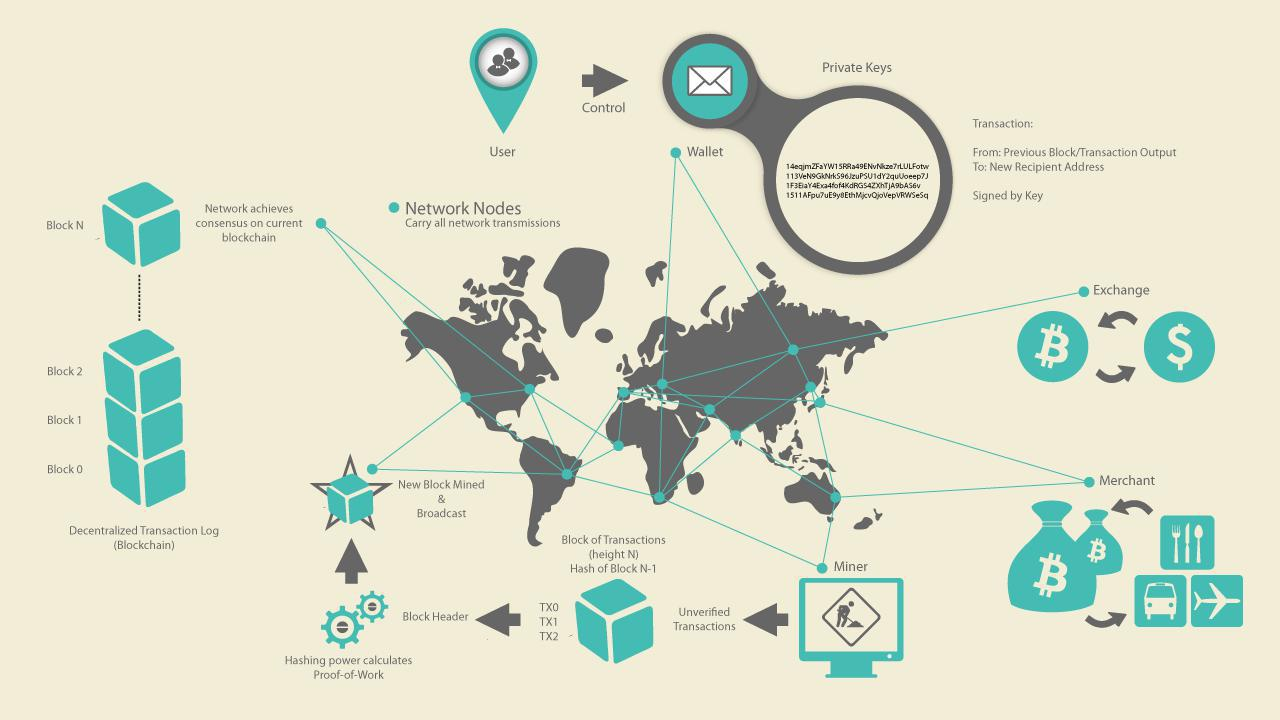
\includegraphics[width=1\columnwidth]{bitcoin} 
	\caption[Panoramica su bitcoin]{Panoramica su bitcoin}
	\label{fig:panoramica-bitcoin} 
\end{figure}
Procedendo nella lettura si troveranno degli esempi di transazioni che sono state effettivamente eseguite sul network, ma che verranno associate a virtuali interazioni tra attori come Alice, Bob e Joe. Per tracciare una transazione in particolare attraverso il network bitcoin e la blockchain, si può utilizzare un blockchain explorer, piattaforma online che opera come un motore di ricerca bitcoin. Questi servizi permettono di cercare per indirizzo, transazione e per blocco e vedere i relativi flussi all'interno di questi.
Tra i Blockchain Explorers più conosciuti troviamo:
\begin{itemize}
	\item Blockchain info https://www.blockchain.com/explorer
	\item Bitcoin Block Explorer https://blockexplorer.com/
	\item Insight https://insight.bitpay.com/
	\item Coinbase https://www.coinbase.com/
\end{itemize} 
Ma vediamo una panoramica del sistema bitcoin, vedi Figura \ref{fig:panoramica-bitcoin}, notiamo che tale sistema è composto di utenti con i propri portafogli (\textit{wallet}) che contengono delle chiavi (\textit{key}), le transazioni si propagano attraverso il network, i miner producono, tramite una gara di computazione, la blockchain del consenso che rappresenta il libro mastro autoritativo di tutte le transazioni.

\subsection{Transazioni Bitcoin}
Una transazione comunica la network che il proprietario di un certo numero di bitcoin ha autorizzato il trasferimento di una parte di essi ad un altro proprietario. Quando tutta l'operazione andrà a buon fine il nuovo proprietario potrà spendere questi bitcoin e di conseguenza spenderli creando una nuova transazione verso un altro utente. Tutto questo genera una catena di passaggi di proprietà.
\begin{figure}
	\centering 
	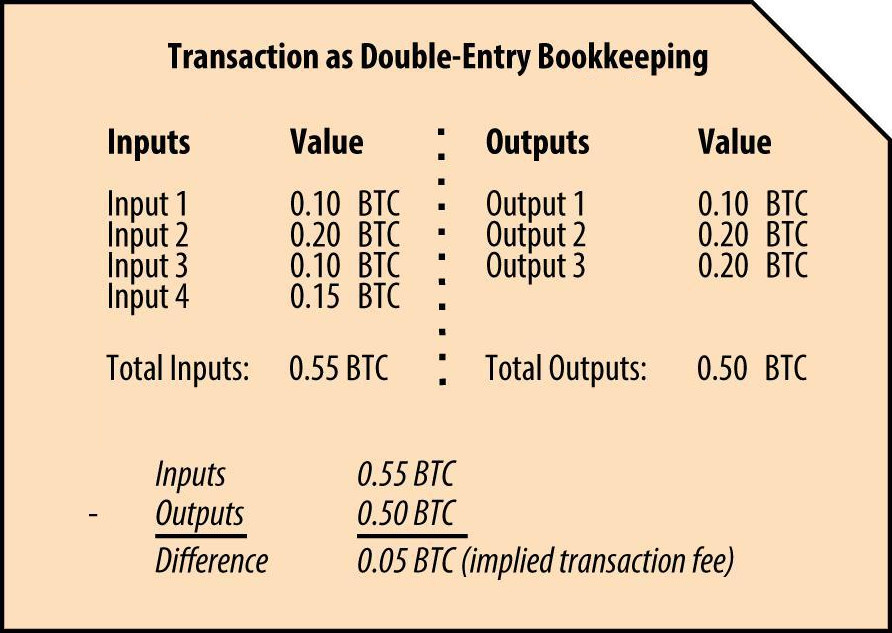
\includegraphics[width=.6\columnwidth]{double-entry-transaction} 
	\caption[Double entry transaction]{Double entry transaction}
	\label{fig:double-entry-transaction} 
\end{figure}
Ogni transazione può contenere uno o più \textit{input}, che sono i debiti verso un account bitcoin. Dall'altro lato della transazione ci sono uno o più \textit{output}, che rappresentano i crediti aggiunti ad un account bitcoin, vedi Figura \ref{fig:double-entry-transaction}. Gli \textit{input} e gli \textit{output} se sommati non totalizzano necessariamente lo stesso risultato. Al contrario, gli \textit{output} risultano poco inferiori rispetto a quello degli \textit{input} e tale differenza rappresenta la \textit{Transaction fee} o Commissione di Transazione sottintesa, che è un piccolo pagamento che il miner ottiene includendo la transazione all'interno del registro. 
\begin{figure}
	\centering 
	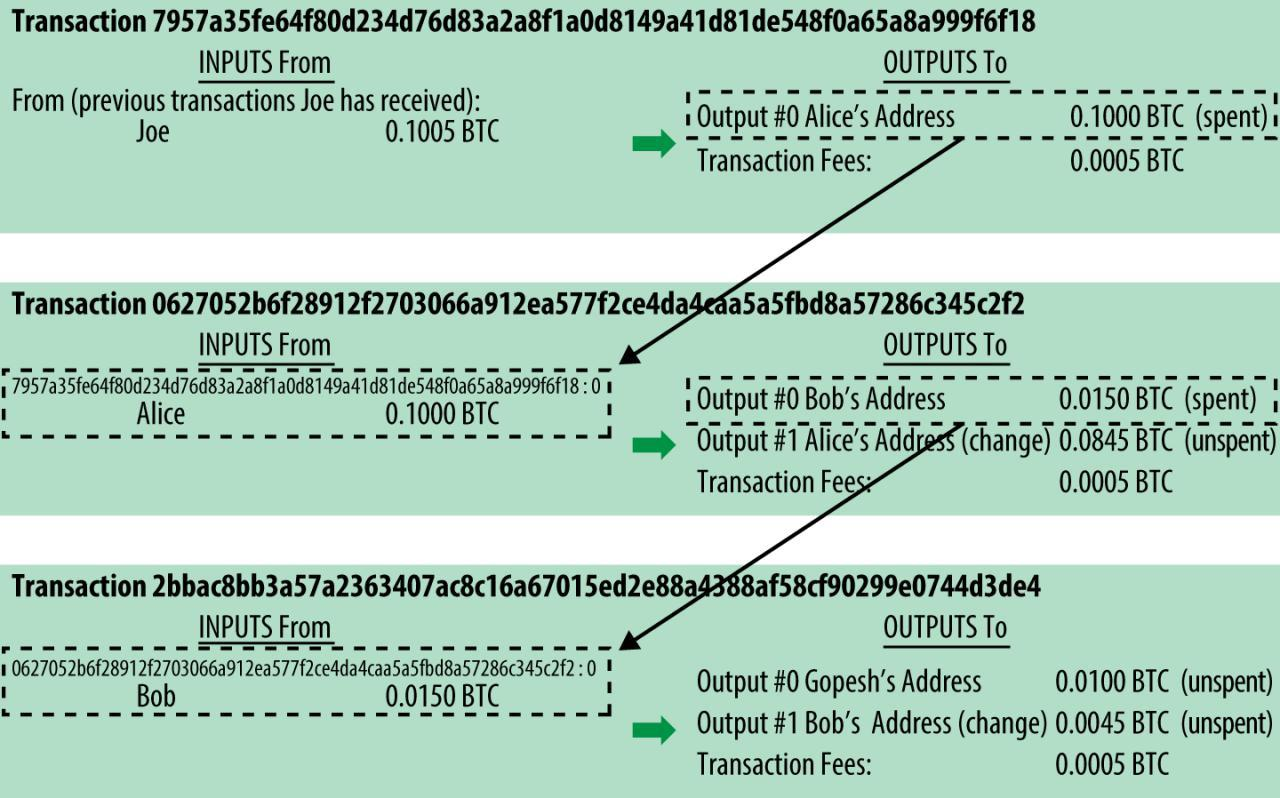
\includegraphics[width=1\columnwidth]{catena-di-transazioni} 
	\caption[Catena di transazioni]{Catena di transazioni}
	\label{fig:catena-di-transazioni} 
\end{figure}
Nella sezione precedente illustravamo come un nuovo potenziale utente potesse ricevere bitcoin in cambio di denaro. Era il caso di Alice e Joe. Tale transazione ha un numero di bitcoin bloccati attraverso la chiave di Alice. Il pagamento che ora Alice intende fare a Bob fa riferimento alla transazione precedente come un input e crea nuovi output per pagare la somma dovuta e per ricevere il resto. Questa rappresenta una vera e propria catena, nella quale gli input dell'ultima transazione corrispondono agli output delle transazioni precedenti. La chiave di alice fornisce la firma che sblocca questi importi in output delle precedenti transazioni, provando a tutta la network che lei è la legittima proprietaria di quei fondi, un esempio di catena la si può vedere in figura \ref{fig:catena-di-transazioni}.

\subsection*{Tipologie di transazione}
Ci sono vari tipi di transazione in base alla quantità di input e output all'interno di essa. Ma vediamoli nel dettaglio:
\begin{itemize}
	\item \textbf{Common Transaction:} la forma più comune di transazione, spesso include un resto e viene ritornato al proprietario originario. Questo tipo di transazione ha un solo input e due output.
	\item \textbf{Aggregating Transaction:} aggrega multipli input in un singolo output. Questa operazione nel mondo reale equivale allo scambiare una pila di monete e banconote per una banconota singola di valore maggiore. Viene comunemete utilizzata per far pulizia da transazioni di valore piccolo, ricevute come resto di numerosi pagamenti precedenti.
	\item \textbf{Distributing Transaction:} transazione che distribuisce un input a più di un outputche rappresentano multipli destinatari. Questo tipo di transazione è talvolta usato dagli esercizi commerciali per distribuire i guadagni, ad esempio quando l'azienda effettua il pagamento degli stipendi ai vari dipendenti.
\end{itemize}

\subsection{Costruire una transazione}
L'applicazione wallet di Alice contiene un'apposita logica che fa in modo di selezionare gli appropriati input e output per costruire una transazione secondo le specifiche imposte da Alice che dovrà solamente specificare una destinazione e l'importo desiderato, il resto viene fatto dall'applicazione.

\subsection*{Ottenere gli input giusti}
L'applicazione wallet di alice deve essere in grado di comporre una transazione inserendo gli input, intesi come frammenti di bitcoin che le appartengono, del valore che intende inviare come pagamento a Bob.Le varie tecniche per fare ciò dipendono dalla tipologia di client che Alice possiede oppure dal fatto che tenga aggiornato un'indice completo dei propri unspent output di ogni transazione nella blockchain. Nel caso Alice non mantenga aggiornato un indice del genere, ha comunque la possibilità di ricavare tale insieme di unspent bitcoin tramite svariate API anche utilizzando un semplice client HTTP. 
\begin{lstlisting}
{
 "unspent_outputs":[
  {
   "tx_hash":"186f9f998a5...2836dd734d2804fe65fa35779",
   "tx_index":104810202,
   "tx_output_n": 0,
   "script":"76a9147f9b1a7fb68d60c536c2fd8...f3cc025a888ac",
   "value": 10000000,
   "value_hex": "00989680",
   "confirmations":0
  }
 ]
}
\end{lstlisting}
Quella mostrata nel riquadro qui sopra risulta la risposta ad una possibile richiesta da parte di Alice che contiene un unspent output. Viene riportata anche la referenza alla transazione nella quale questo unspent bitcoin è contenuto e il relativo valore in bitcoin, 10 milioni, equivalente a 0.10 BTC. Con questa informazione il wallet di Alice potrà costruire una transazione utilizzando questo valere come input e quindi trasferire quel valore all'indirizzo del nuovo proprietario.\\
\textbf{NB:} In questo caso il wallet di Alice dispone di un unspent output con abbastanza bitcoin che riesce a coprire la sua spesa. In alcuni casi può succedere di non disporre di un unico unspent output che riesce a coprire il debito da saldare. In questi casi si dovrà procedere con l'inserimento all'interno della transazione di altri unspent output fino a coprire la spesa da sostenere. In ogni caso Alice dovrà attendersi del resto ma quello lo vedremo nella prossima sezione.

\subsection*{Creare gli output}
La transazione che sta per creare Alice, oltre agli input, include almeno un nuovo output che sarà creato facendo in modo che possa essere riscattato solamente dal legittimo proprietario, in questo caso Bob. Tutto ciò è possibile creando l'output in questione sotto forma di script che creerà un blocco sul valore e potrà essere riscattato solamente da chi sottoporrà una soluzione, in questo caso ci si aspetta la firma della chiave corrispondente all'indirizzo pubblico di Bob. Solo il wallet di Bob potrà presentare una simile firma dal momento che è il creatore di tale chiave pubblica. 
Questa transazione inoltre dovrà includere un'ulteriore output, dal momento in cui i fondi di Alice sono nella forma di un output di 0.10 BTC, un valore elevato se paragonato al pagamento di una cifra d'esempio di 0.015 BTC. In questo caso ad alice spetterebbero 0.085 BTC di resto. Questa cifra andrà rappresenta il secondo output della transazione che sarà indirizzato ad Alice.
Infine, per fare in modo che il network processi la transazione in tempi ragionevoli, l'applicazione wallet di Alice aggiungerà una piccola commissione di transazione (fee). Questa non viene esplicitata nella transazione ma è data dalla differenza tra gli input e gli output, quindi se Alice imposterà l'output resto a 0.0845 BTC avanzeranno 0.0005 BTC. Questa transaction fee sarà recuperata dal miner come commissione per aver incluso la transazione all'interno di un blocco e averla scritta all'interno del registro blockchain. La transazione risultante, una volta confermata ed inviata sul network, può essere vista utilizzando un'applicazione web del tipo blockchain explorer, vedi Figura \ref{fig:transazione-alice-bob}.
\begin{figure}
	\centering 
	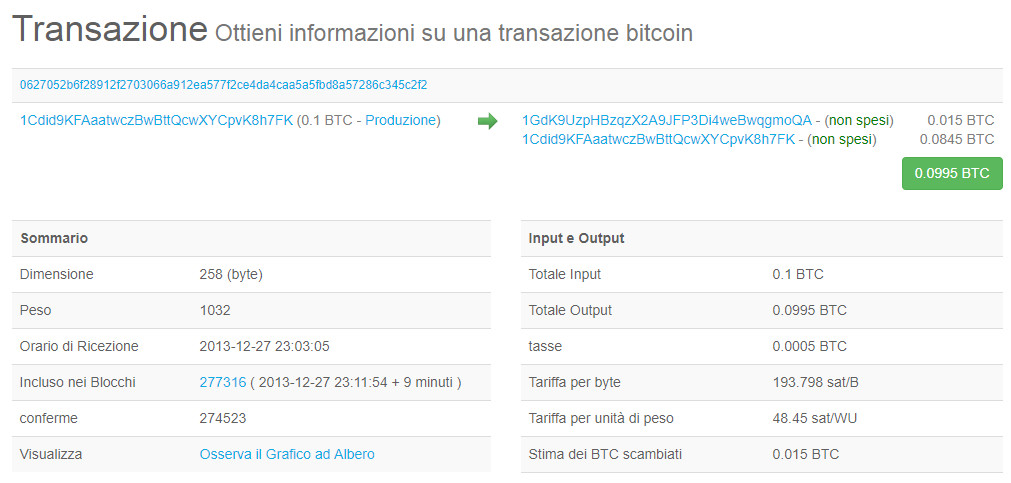
\includegraphics[width=1\columnwidth]{transazione-alice-bob} 
	\caption[Transazionte tra Alice e Bob]{Transazionte tra Alice e Bob}
	\label{fig:transazione-alice-bob} 
\end{figure}

\subsection*{Aggiungere la transazione al Ledger}
In questo momento la transazione tra Alice e Bob viene inviata al network e, come vediamo in Figura \ref{fig:transazione-alice-bob}, risulta avere una grandezza di 258 byte. Come abbiamo visto, all'interno di essa troviamo tutto il necessario per confermare la proprietà dei fondi e assegnare loro nuovi proprietari. La presenza di tutte informazioni danno modo a Bob di verificare fin da subito la transazione controllando che gli input utilizzati corrispondano a precedenti unspent output oltre a verificare che gli importi, comprese le fee, siano adeguati. Bob dovrà aspettare in media 10 minuti per vedere la propria transazione come \textit{confermata}, quindi inserita all'interno del Ledger.

\section{Il Mining di Bitcoin}
Una transazione non entra a far parte del libro mastro condiviso (blockchain) fino a che non viene verificata ed inclusa in un blocco da un processo chiamato \textit{mining}. Il processo di mining in bitcoin serve a due scopi:
\begin{itemize}
	\item Il processo di mining genera nuovi bitcoin per ogni blocco. La quantità di bitcoin creata per ogni blocco è fissa e diminuisce col passare degli anni.
	\item Il mining genera fiducia assicurando che le transazioni siano confermate solo se è stata usata una sufficiente potenza di calcolo. Il problema da risolvere è basato su di un hash crittografico.
\end{itemize}
Ogni 10 minuti un miner entra a far parte di una competizione globale tra miners, alla ricerca di una soluzione per un blocco di transazioni. Trovare tale soluzione, chiamata \textit{proof-of-work}, richiede decine di miliardi di operazioni hash al secondo in tutta la rete bitcoin. L’algoritmo di \textit{proof-of-work} comporta l’effetuare ripetutamente un’operazione di hashing dell’header del blocco e un numero casuale con
l’algoritmo crittografico SHA256 fino a che non emerga una soluzione corrispondente a un determinato pattern. Il primo miner a trovare tale soluzione vince il round della competizione e pubblica il blocco nella blockchain, aggiudicandosi dei bitcoin nuovi di zecca.

Al momento della scrittura di questa Tesi  la difficoltà di questi problemi è così alta da rendere redditizio effettuare mining solamente con circuiti integrati specifici per l'applicazione selezionata\footnote{ASIC, Application Specific Integrated Circuits}, nel nostro caso si tratta di centinaia di algoritmi di mining direttamente stampati su chip hardware, eseguito poi in parallelo su di un singolo chip in silicio. Un miner puù far parte di una mining-pool nella quale i partecipanti dividono gli sforzi e i proventi.

\subsection*{Mining delle Transazioni presenti nei Blocchi}
Una transazione trasmessa attraverso il network bitcoin non è verificata fino a quando non viene inglobata all'interno di un blocco che verrà inserito sulla cima della blockchain, questo accade in media ogni 10 minuti. Nuove transazione fruiscono costantemente nel network da wallet utente e altri applicativi, non appena queste vengono notate dai vari manier verranno aggiunte ad una pool temporanea di transazioni non verificate, pool mantenuta da ogni singolo nodo. Mano a mano che i miner cercano di comporre un nuovo blocco vanno a verificare e quindi ad aggiungere nuove transazioni al blocco su cui lavorano, dando priorità alle transazioni la cui fee risulta più alta. Ogni miner inizia il processo di mining di un blocco di transazioni nel momento in cui riceve il blocco precedente dal network, prendendo atto di aver perso l'ultimo round della competizione. Il miner crea immediatamente un nuovo blocco, lo riempie con transazioni e con le informazioni (l’hash) del blocco precedente, e inizia a calcolare la proof of work per il nuovo blocco. Ogni miner include una transazione speciale nel suo blocco, una che paga al proprio indirizzo bitcoin una ricompensa per i nuovi bitcoin creati (attualmente 12.5 BTC per blocco). Se il miner trova una soluzione che rende il blocco valido, egli "vince" questa ricompensa perchè il suo
blocco "vincente" è aggiunto alla blockchain globale e la transazione di ricompensa che lui ha incluso in esso diventa spendibile. Supponendo che il miner Jing vinca la competizione, lui andrà a diffondere nel network il nuovo blocco, \texttt{\#277316}, contenente 419 altre transazioni. Alla ricezione di questo blocco gli altri miner lo validano e iniziano a contendersi la generazione del blocco successivo. Qualche minuto più tardi un altro miner troverà una soluzione per il successivo blocco, \texttt{\#277317} che andrà a posizionarsi sulla cima della blockchain. Dal momento in cui questo nuovo blocco è basato sul blocco precedente, che conteneva la transazione di alice, ha aggiunto una grande quantità di computazione su quel blocco, rafforzando quindi la fiducia riposta in tutte le transazioni presenti nel blocco \texttt{\#277316}. Man mano che i blocchi si impilano uno sopra l’altro, diventa esponenzialmente più difficile invertire la transazione, rendendo il network sempre più sicuro. Questo aspetto lo si può notare graficamente nella Figura \ref{fig:blockchain-277316} dove vediamo il blocco \texttt{\#277316}, contenente la transazione di Alice, al di sotto del quale troviamo 277316 blocchi fino, infatti ad arrivare al blocco \texttt{\#000000}, conosciuto anche come \textit{genesis block}. Per convenzione, ogni blocco con più di 6 conferme è considerato irrevocabile dal momento in cui si necessiterebbe di un'ammontare immenso di computazione per invalidarlo e di conseguenza revocare anche i successivi sei blocchi.
\begin{figure}
	\centering 
	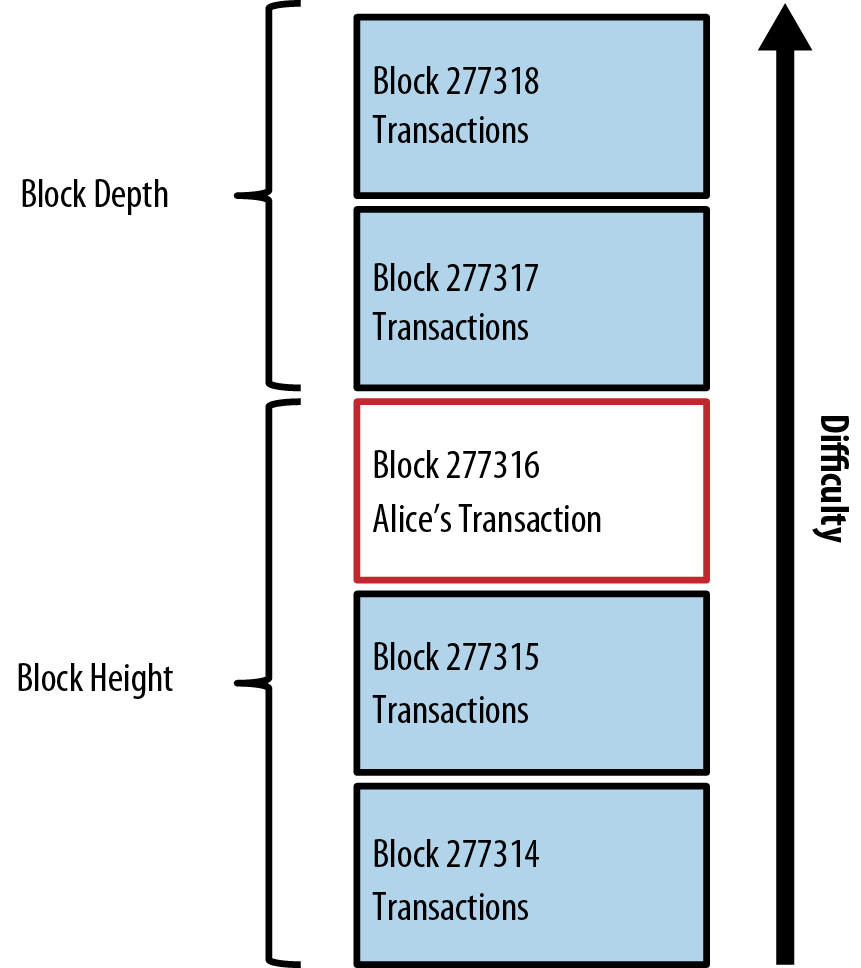
\includegraphics[width=.5\columnwidth]{blockchain-277316} 
	\caption[Transazionte di Alice inclusa nel blocco \texttt{\#277316}]{Transazionte di Alice inclusa nel blocco \texttt{\#277316}}
	\label{fig:blockchain-277316} 
\end{figure}
Da questo punto in poi la transazione di Alice è stata inclusa nella blockchain e sarà visibile a tutte le applicazioni bitcoin. Ogni client bitcoin può verificare indipendentemente la transazione come valida e spendibile. Sarà in oltre possibile tracciare a ritroso il percorso completo del denaro fino alla fonte.

\section{Chiavi, Indirizzi e Wallet}
La proprietà dei bitcoin si stabilisce attraverso chiavi digitali, indirizzi bitcoin e firme digitali. Le chiavi digitali sono create e mantenuti dai vari utenti in un file o database chiamato wallet. Le chiavi digitali nel wallet di un utente sono completamente indipendenti dal protocollo bitcoin e possono essere generate e gestite dal software del wallet dell’utente senza alcuna relazione con la blockchain o accesso a Internet. Esse consentono molte delle interessanti proprietà dei bitcoin, incluso controllo e fiducia de-centralizzata.

Ogni transazione bitcoin richiede una firma valida per essere inclusa nella blockchain, che può essere generata solo con chiavi digitali valide; pertanto, chiunque disponesse di una copia di quelle chiavi ha il controllo del bitcoin in quel conto. Si tratta di coppie di chiavi composte da una chiave privata, che deve rimanere segreta, e una chiave pubblica. Sono in genere memorizzate all'interno del file del wallet e vengono gestite dal relativo software. 

Nella parte di pagamento di una transazione bitcoin, la chiave pubblica del destinatario è rappresentata dalla sua impronta digitale, chiamata indirizzo bitcoin, che viene utilizzata allo stesso modo del nome del beneficiario su un assegno. Nella maggior parte dei casi, un indirizzo bitcoin generato corrisponde ad una chiave pubblica. Tuttavia, non tutti gli indirizzi bitcoin rappresentano chiavi pubbliche; possono anche rappresentare altri beneficiari come gli script, che vedremo più avanti.

\subsection{La Crittografia a Chiave Pubblica e le Criptovalute}
La crittografia a chiave pubblica è stata inventata negli anni '70 (1970) ed è una delle basi matematiche dei computer e della sicurezza informatica.
Da quando stata inventata la crittografia a chiave pubblica, sono state scoperte diverse funzioni matematiche idonee, come ad esempio l’elevazione a potenza dei numeri primi e la moltiplicazione a curva ellittica. Queste funzioni matematiche sono praticamente irreversibili, nel senso che sono facili da calcolare in una direzione e risulta essere molto difficili da calcolare nella direzione opposta. Sulla base di queste funzioni matematiche, la crittografia consente la creazione di segreti digitali e firme digitali non falsificabili. Bitcoin usa la moltiplicazione a curva ellittica come base per la sua crittografia a chiave pubblica.
In bitcoin, usiamo la crittografia a chiave pubblica per creare una coppia di chiavi che controlla l’accesso ai bitcoin. La coppia di chiavi consiste di una chiave privata e un’unica chiave pubblica, l'una derivata dall'altra. La chiave pubblica è usata per ricevere bitcoin, e la chiave privata è usata per autorizzare transazioni per spenderli. C’è una relazione matematica tra la chiave pubblica e quella privata che permette alla chiave privata di essere usata per generare firme sui messaggi. Questa firma può essere validata attraverso la chiave pubblica senza rivelare la chiave privata.
Nella maggior parte delle implementazioni di wallet, le chiavi privata e pubblica sono
salvate insieme come coppia di chiavi per convenienza. Comunque, la chiave pubblica
può essere ricavata dalla chiave privata, quindi è possibile salvare anche solo la
chiave privata.
Un portafoglio bitcoin contiene una raccolta di coppie di chiavi, ognuno composto da una chiave privata e una chiave pubblica. Vediamo come vengono generate queste chiavi:
\begin{itemize}
	\item La chiave privata (k) è un numero, di solito scelto a caso.
	\item Dalla chiave privata, viene utilizzata la curva ellittica, una funzione di crittografia unidirezionale, per generare una chiave pubblica (K).
	\item Dalla chiave pubblica (K), viene utilizzata una funzione di hash crittografica unidirezionale per generare un indirizzo bitcoin (A).
\end{itemize}
La rappresentazione grafica di tutto questo lo si può vedere in Figura \ref{fig:pk-sk-indirizzo-bitcoin}.
\begin{figure}
	\centering 
	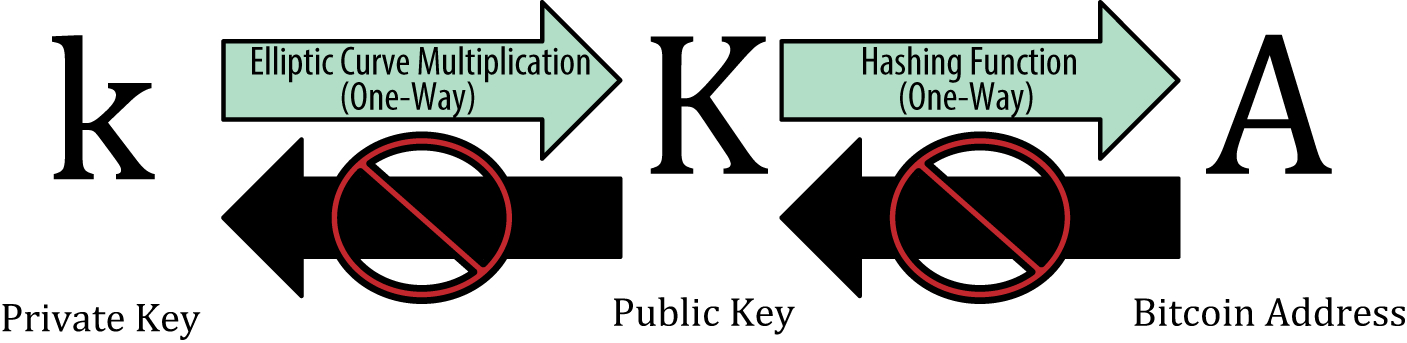
\includegraphics[width=1\columnwidth]{pk-sk-indirizzo-bitcoin} 
	\caption[Chiave privata, chiave pubblica e indirizzo bitcoin]{Chiave privata, chiave pubblica e indirizzo bitcoin}
	\label{fig:pk-sk-indirizzo-bitcoin} 
\end{figure}

\subsubsection{Le chiavi private}
Come abbiamo visto poco fa, una chiave privata è semplicemente un numero scelto casualmente. E' utilizzata per creare le firme necessarie per trasferire i bitcoin, con lo scopo di dimostrare la proprietà dei fondi utilizzati nella transazione. La chiave privata deve essere:
\begin{itemize}
	\item \textbf{Segreta:} rivelarla a terzi equivarrebbe a dare loro il controllo dei bitcoin associati a tale chiave.
	\item \textbf{Protetta da perdite:} deve infatti essere conservata e protetta da perdite accidentali, se questo accadesse i fondi associati ad essa saranno anch'essi persi per sempre.
\end{itemize}
Il primo e più importante passo per generare chiavi è quello di trovare una fonte sicura di entropia, scegli un numero tra $1$ e $2^{256}$. Il metodo utilizzato per la selezione di tale numero non risulta importante fintanto che non sia prevedibile. Il software attuale utilizza il generatore di numeri casuali fornito dall'OS inizializzato però da una fonte esterna di casualità. Più precisamente, la chiave privata potrebbe essere un qualsiasi numero tra $1$ e $n-1$, dove $n$ è una costante ($n=1.158*10^{77}$, un po' meno di $2^{256}$), definito come ordine di curvatura della curva ellittica usata in bitcoin. Si sceglierà un numero casuale di 256 bit inferiore di $n-1$. Questo avviene eseguendo l'algoritmo SHA256 su di una stringa casuale $s$ dove $|s|>256$ bit, questo produrrà comunque un numero di 256 bit. Se tale numero risulterà inferiore di $n-1$ verrà accettato, altrimenti si ripeterà l'algoritmo con un input diverso. La seguente è una chiave privata casuale $k$ mostrata nella sua rappresentazione esadecimale (256 cifre mostrate come 64 cifre esadecimali, ognuna da 4 bit):
\[\text{\small 1E99423A4ED27608A15A2616A2B0E9E52CED330AC530EDCC32C8FFC6A526AEDD}\]
Per generare una nuova chiave tramite il client Bitcoin Core, si utilizza il comando $getnewaddress$. Per ragioni di sicurezza verrà mostrata solamente la chiave pubblica. E' comunque possibile chiedere a Bitcoin Core  di esporre anche le chiave privata tramite il comando $dumpprivkey$ che la mostrerà in formato Base58 checksum-encoded chiamato anche \textit{Wallet Import Format} (WIF).
\begin{lstlisting}
$ bitcoind getnewaddress
 1J7mdg5rbQyUHENYdx39WVWK7fsLpEoXZy
$ bitcoind dumpprivkey 1J7mdg5rbQyUHENYdx39WVWK7fsLpEoXZy
 KxFC1jmwwCoACiCAWZ3eXa96mBM6tb3TYzGmf6YwgdGWZgawvrtJ
\end{lstlisting}
\texttt{NB:} Il comando \textit{dumpprivkey} non genera una chiave privata da una chiave pubblica, visto che è impossibile. Il comando semplicemente rivela la chiave privata che è già conosciuta al wallet e che è stata generata dal comando \textit{getnewaddress}.

\subsubsection{Le chiavi pubbliche}
La chiave pubblica è calcolata da quella privata utilizzando la proprietà di moltiplicazione delle curve ellittiche, operazione irreversibile: $K=k*G$ dove $k$ è la chiave privata, $G$ è un punto costante della curva ellittica chiamato \textit{Generator Point} e $K$ sarà la chiave pubblica risultante. L'operazione inversa, conosciuta come trovare il logaritmo discreto, calcolando $k$ conoscendo $K$, risulta difficile come provare per tutti i possibili valori di $k$, brute-force search.

\subsubsection{Crittografia e Curve Ellittiche}
Le curve ellittiche in crittografia sono un tipo di crittografia assimmetrica, utilizzano coppie di chiavi $(Pk, Sk)$, basata sul problema del logaritmo discreto. La curva utilizzata da bitcoin è definita in uno standard detto \textit{secp256k1} dal National Institute of Standards and Technology (NIST). La \textit{secp256k1} è definita dalla seguente funzione:
\[  y^{2}=(x^{3}+7) \text{ over } (\mathbb{F}_{p}) \quad \text{ or } \quad y^{2} \bmod p=(x^{3}+7) \bmod p\]
Il $\bmod p$ indica che questa curva è su di un campo finito di numeri primi di ordine $p$, ch possiamo definire come $\mathbb{F}_{p}$ dove $p = 2^{256} - 2^{32} - 2^{9} - 2^{8} - 2^{7} - 2^{6} - 2^{4} - 1$, in parole povere, un numero primo molto grande.
Nella matemetica delle curve ellittiche c'è un punto chiamato \textit{point as infinity}, il quale viene fatto corrispondere allo zero nell'addizione.
Esiste un operatore $+$, chiamato addizione che dati due punti $P_{1}$ e $P_{2}$ sulla curva ellittica, $\exists P_{3} \quad | \quad P_{3} = P_{1} + P_{2}$. Geometricamente, questo nuovo punto $P_{3}$ viene calcolato tracciando una linea tra $P_{1}$ e $P_{2}$. Questa linea intersecherà la curva ellittica nel punto addizionale chiamato appunto $P_{3} = (x, y)$. Tale punto lo possiamo riflettere sull'asse delle $x$ ottenendo $P_{3} = (x, -y)$. Esistono vari casi particolari di queste addizioni tra punti, se il lettore ne fosse interessato è consigliata la lettura dei testi \cite{mastering:andreas} e \cite{mastering2:andreas}.

\subsubsection{Generazione della chiave pubblica}
Partendo da una chiave privata $k$, numero generato casualmente, lo moltiplichiamo con un punto predeterminato sulla curva, denominato \textit{generator point} $G$ producendo un ulteriore punto situato in qualche altra parte della curva. Questo punto sarà la chiave pubblica $K$. 
\[ K=k*G\]
Poiché il punto di generazione $G$ è sempre lo stesso per tutti gli utenti di bitcoin, una chiave privata $k$ moltiplicata per $G$ darà sempre come risultato la stessa chiave pubblica $K$. La relazione tra $k$ e $K$ è fissa, ma può essere calcolata in una sola direzione.
\[ k \Rightarrow K \quad k \nLeftarrow K\]
Per questo motivo la chiave pubblica, $K$, di un utente può essere condivisa con chiunque senza rivelare alcuna informazione circa la relativa chiave privata, $k$.
Moltiplicare $G$ per un qualsiasi numero $k$ equivale ad aggiungere $G$ a se stesso $k$ volte di seguito. Nelle curve ellittiche, aggiungere un punto a se stesso equivale a tracciare una linea tangente al punto e trovare quindi dove questa interseca nuovamente la curva, infine riflettiamo questo punto sull'asse delle $x$. La dimostrazione grafica di queste operazioni eseguite in modo consecutivo lo troviamo in Figura \ref{fig:crittografia-ellittica}.
\begin{figure}
	\centering 
	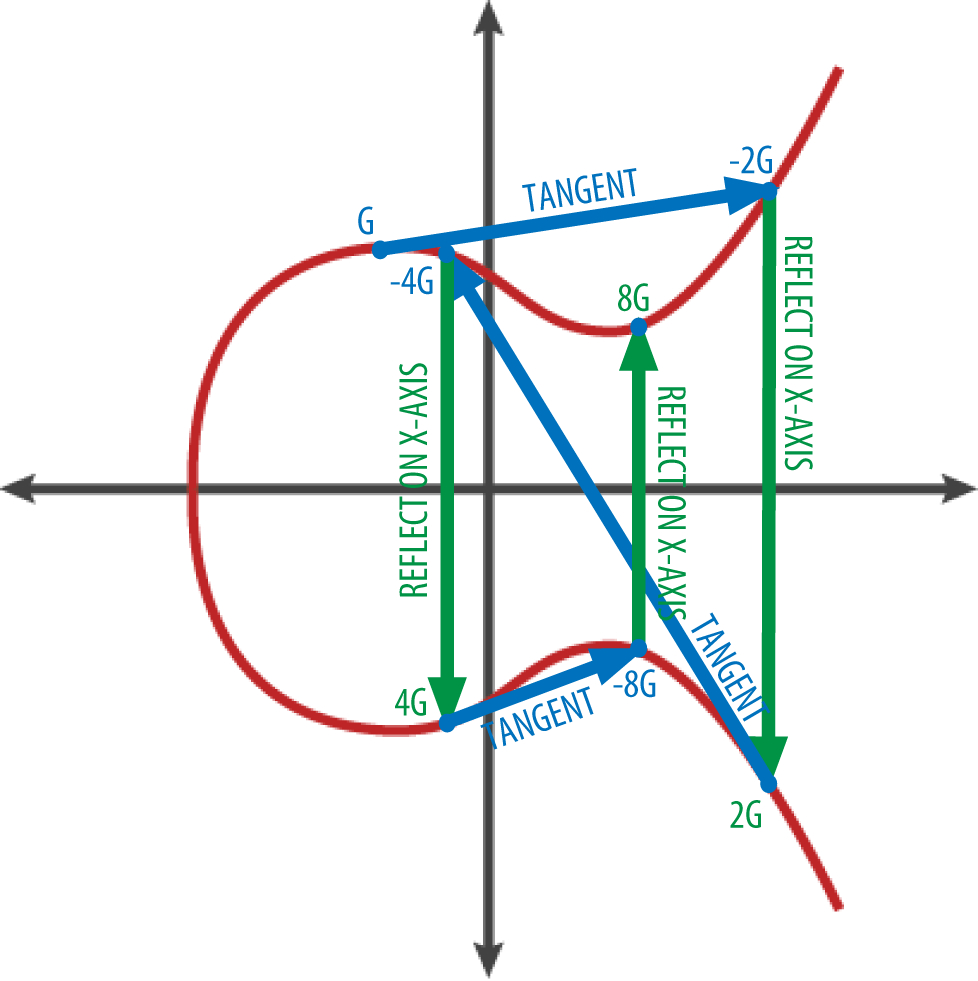
\includegraphics[width=.6\columnwidth]{crittografia-ellittica} 
	\caption[Crittografia Ellittica]{Schema di funzionamento della moltiplicazione nelle curve ellittiche, $G*k$.}
	\label{fig:crittografia-ellittica} 
\end{figure}

\subsubsection{Indirizzi Bitcoin}
Un indirizzo bitcoin è una stringa di cifre e caratteri che può essere condivisa con chiunque desideri inviarti denaro. Gli indirizzi prodotti dalle chiavi pubbliche sono costituiti da una stringa di numeri e lettere che inizia con $1$. Ecco un esempio di indirizzo bitcoin:
\[ \text{1J7mdg5rbQyUHENYdx39WVWK7fsLpEoXZy} \]
Questo indirizzo è quello che appare comunemente in una transazione come \textit{destinatario} dei fondi. Un indirizzo bitcoin può rappresentare un proprietario di una coppia di chiavi $(Pk,Sk)$, oppure qualcos'altro come uno script di pagamento. 
L'indirizzo bitcoin è derivato dalla chiave pubblica attraverso l'uso di una funzione one-way\footnote{Una funzione one-way è una funzione matematica unidirezionale cioè "facile da calcolare", ma "difficile da invertire"} in questo caso un hashing crittografico. tali funzioni sono usate ampiamente in bitcoin: negli indirizzi bitcoin, negli indirizzi di script e negli algoritmi di \textit{proof-of-work}. Gli algoritmi utilizzato sono in particolare:
\begin{description}
	\item[SHA] (Secure Hash Algorithm) in particolare SHA256.
	\item[RIPEMD] (RACE Integrity Primitives Evaluation Message Digest) in particolare RIPEMD160.
\end{description}
Iniziando dalla chiava pubblica $K$, ne calcoliamo l'hash \textit{SHA256} e successivamente l'hash \textit{RIPEMD160}, producendo un numero a 160 bit (20 byte) chiamato $A$. La rappresentazione grafica di queste fasi la si può vedere in Figura \ref{fig:pk-to-indirizzo-bitcoin}.\\
\texttt{NB:} l'indirizzo bitcoin non è la chiave pubblica. Gli indirizzi bitcoin sono derivati da una chiave pubblica utilizzando una funzione one-way come abbiamo appena visto. Gli indirizzi bitcoin sono quasi sempre presentati agli utenti in una codifica chiamata \textit{Base58Check} che utilizza 58 caratteri ed un checksum per facilitarne la lettura evitando ambiguità proteggendo l'utilizzatore da errori di trascrizione.
\begin{figure}
	\centering 
	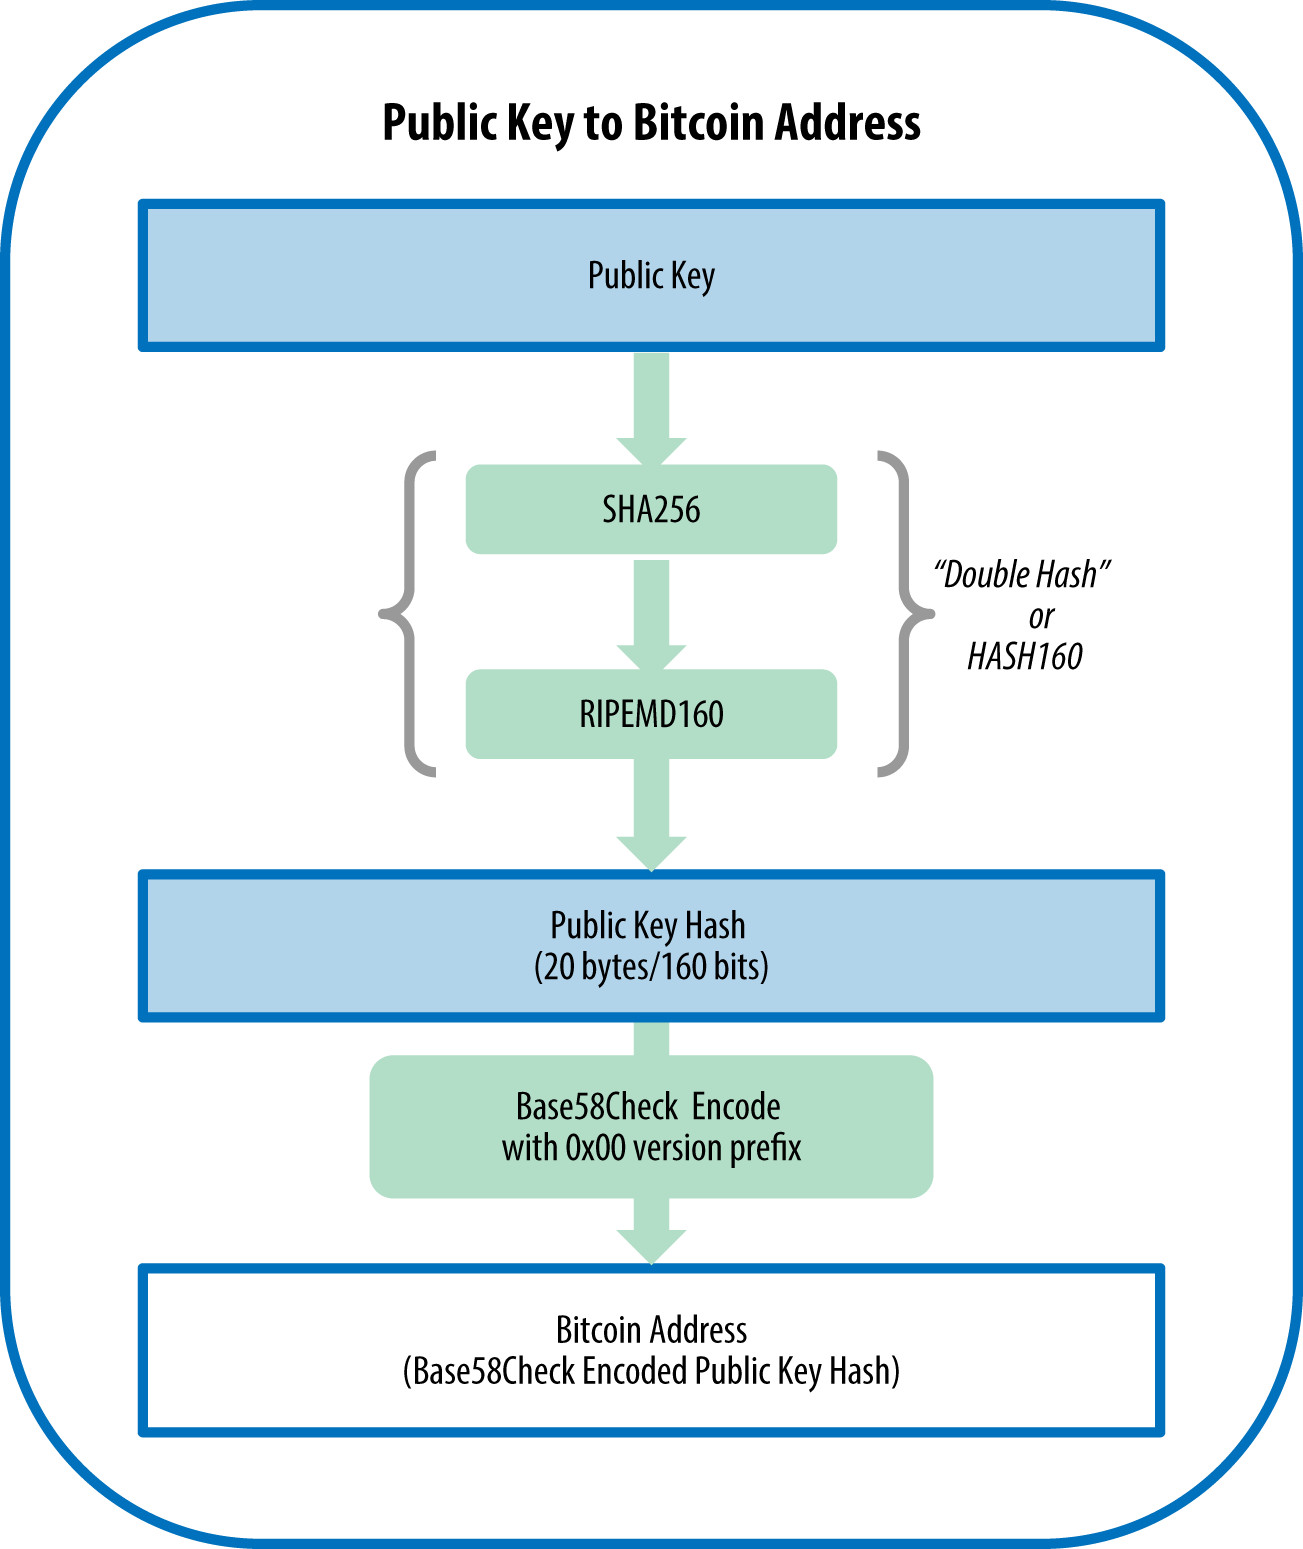
\includegraphics[width=.6\columnwidth]{pk-to-indirizzo-bitcoin} 
	\caption[Da chiave pubblica a indirizzo bitcoin]{Conversione di una chiave pubblica in un indirizzo bitcoin}
	\label{fig:pk-to-indirizzo-bitcoin} 
\end{figure}

\subsection*{I Wallet}
I wallet sono dei contenitori di chiavi private, non monete, solitamente implementati come file strutturati o semplici database. Gli utenti firmano le transazioni con queste chiavi, dimostrando di possedere gli output delle transazioni precedenti, utilizzati come input per le nuove transazioni. La valuta (bitcoin) è memorizzata sulla blockchain sotto forma di transazioni di output.
\subsubsection{Wallet non deterministici}
Nei primi client bitcoin, i wallet erano semplicemente delle raccolte di chiavi private generate casualmente. Questo tipo di portafoglio è chiamato \textit{Type-0 nondeterministic wallet}, sono soprannominati \textit{"Just a Bunch Of Keys"} o JBOK, sono stati sostituiti dai wallet deterministici poiché scomodi da gestire. La scomodità di un wallet non deterministico sta nel fatto che si è obbligati ad eseguire molto spesso dei backup di tutte queste, dato che il loro smarrimento implica la perdita della valuta in bitcoin a cui sono legate. Dato che il riutilizzo degli indirizzi riduce la privacy, si è portati ad una continua generazione di nuove chiavi quindi, per sicurezza, si dovrà rieseguire il backup. Nonostante Bitcoin Core includa un portafoglio di tipo zero, il suo utilizzo è sconsigliato dato che c'è la possibilità di utilizzare un wallet di tipo deterministico. Vedi Figura \ref*{fig:wallet-non-deterministico}.

\subsubsection{Wallet deterministici}
I wallet deterministici sono stati sviluppati per consentire di derivare chiavi multiple da un singolo seme \textit{seed}. La forma più avanzata di questo tipo di wallet è il \textit{hierarchical deterministic wallet} o \textit{HD wallet} definito dallo standard \texttt{BIP0032}, come dice il nome, contengono chiavi derivate in una struttura ad albero tale per cui da ogni chiave madre si possa derivare una sequenza di chiavi figlie e per ognuna di esse si possa derivare una sequenza di chiavi nipote ecc \dots ad una profondità infinita. Tale struttura la possiamo vedere in Figura \ref{fig:wallet-deterministico}
\begin{figure}
	\centering
	\subfloat[][\emph{Wallet non deterministico}]
	{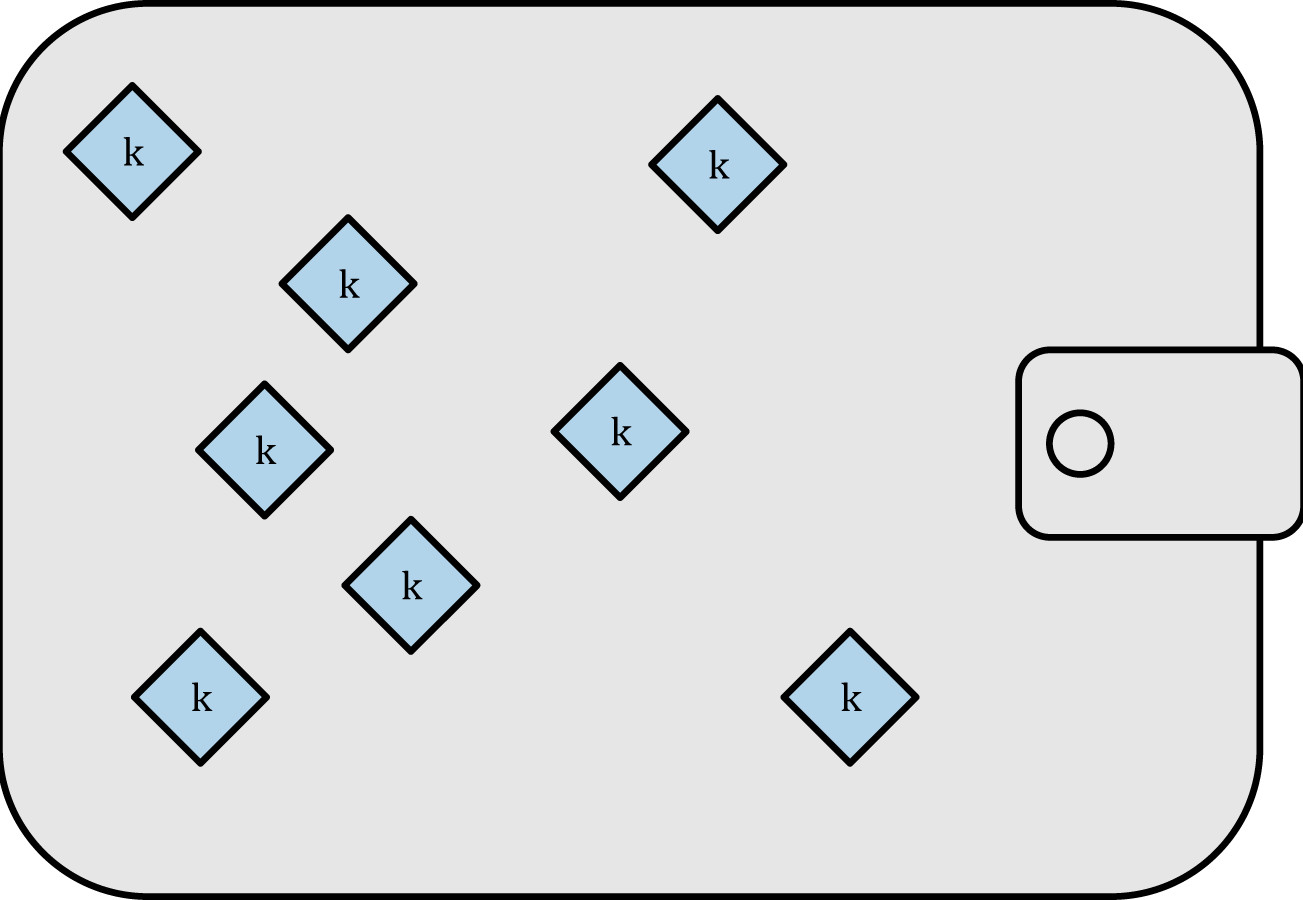
\includegraphics[width=.45\textwidth]{wallet-nondeterministico}
	\label{fig:wallet-non-deterministico}} \quad
	\subfloat[][\emph{Wallet deterministico}]
	{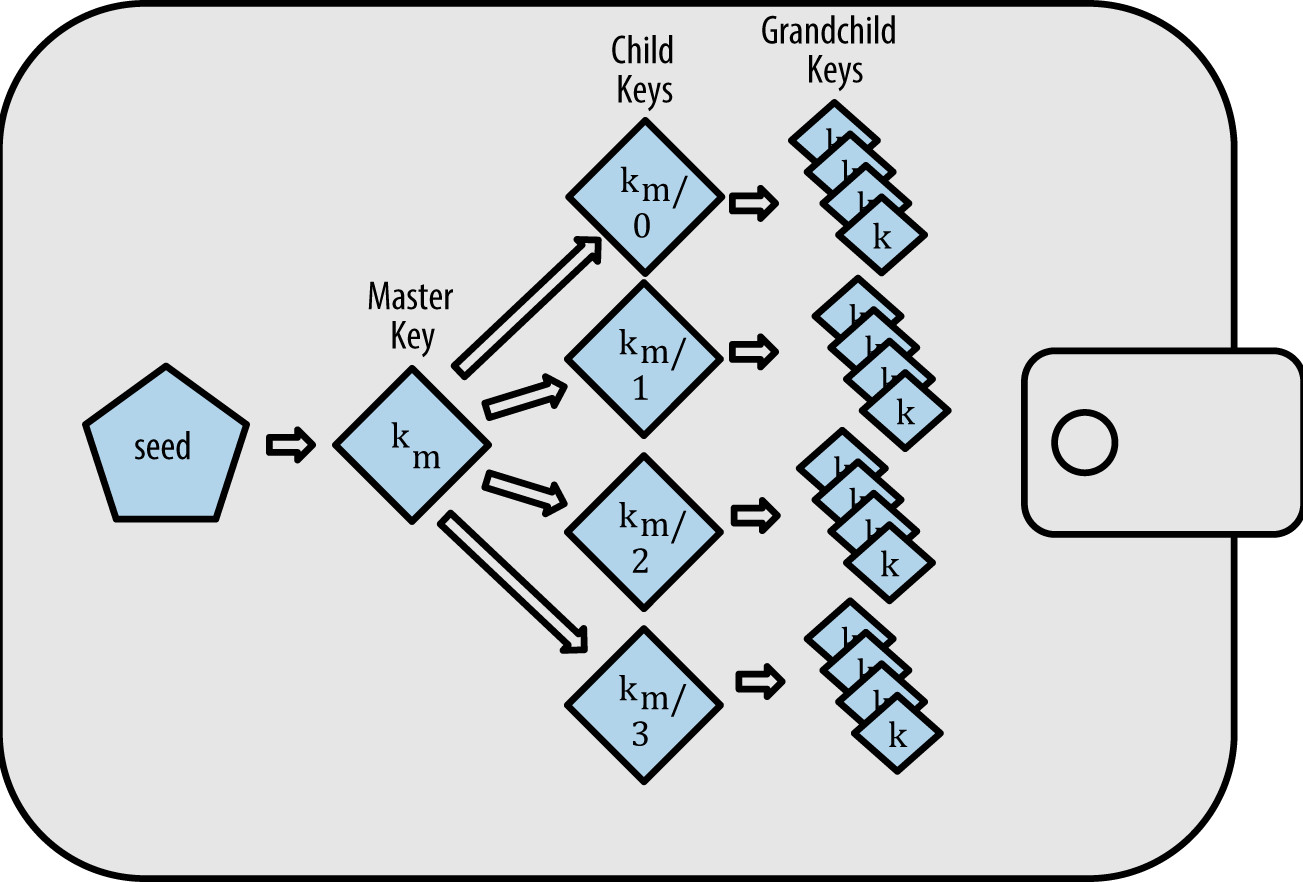
\includegraphics[width=.45\textwidth]{wallet-deterministico}
	\label{fig:wallet-deterministico}}
	\caption{Due tipologie di Wallet}
	\label{fig:tipologie-di-wallet}
\end{figure}
Gli \textit{HD wallet} offrono due importanti vantaggi rispetto alle chiavi casuali.
\begin{itemize}
	\item La struttura ad albero può essere utilizzata per rappresentare una struttura organizzativa aggiuntiva, per esempio alcuni rami potrebbero essere utilizzati per generare chiavi impiegate poi in diversi settori aziendali.
	\item Gli utenti possono creare sequenze di chiavi pubbliche $K_{i}$ senza avere accesso alle corrispettive chiavi private. Questo permette di utilizzare gli HD wallet anche su di un server non sicuro che riuscirà ad emettere una diversa chiave pubblica per ogni transazione.
\end{itemize}

\subsubsection{Vanity Address}
I vanity address sono indirizzi bitcoin validi che contengono dei messaggi mnemonici con un significato per l'uomo. Per esempio \texttt{1LoveBPzzD72PUXLzCkYAtGFYmK5vYNR33} è uno di questi in cui notiamo la presenza della parola \texttt{Love} all'inizio dell'indirizzo. Il processo consiste essenzialmente nel selezionare una chiave privata a caso,derivando la chiave pubblica, derivando l’indirizzo bitcoin e verificando se corrisponde al modello di vanità desiderato, ripetendo miliardi di volte fino a che non verrà trovata una corrispondenza. Questa tipologia di indirizzi non sono più sicuri di qualsiasi altro indirizzo, dipendono dalla stessa Elliptic Curve Cryptography (ECC) e Secure Hash Algorithm (SHA) come qualsiasi altro indirizzo.
\begin{table}[]
	\centering
	\begin{tabular}{|c|c|c|c|c|}
		\hline
		\textbf{Dim.} 	& \textbf{Pattern} 	& \textbf{Frequenza} 		& \textbf{Tempo medio} \\ \hline
		1 			& 1K 		& 1 su 58 chiavi 	& < 1 millisecondi \\ \hline
		2 			& 1Ki 		& 1 su 3,364 		& 50 millisecondi \\ \hline
		3 			& 1Kid 		& 1 su 195,000 		& < 2 secondi \\ \hline
		4 			& 1Kids 	& 1 su 11 million 	& 1 minuto \\ \hline
		5 			& 1KidsC 	& 1 su 656 milioni 	& 1 ora \\ \hline
		6 			& 1KidsCh 	& 1 su 38 miliardi 	& 2 giorni \\ \hline
		7 			& 1KidsCha 	& 1 su 2.2 mila miliardi 	& 3–4 mesi \\ \hline
		8 			& 1KidsChar & 1 su 128 mila miliardi 	& 13–18 anni \\ \hline
		9 			& 1KidsChari 	& 1 su 7 milioni di miliardi	& 800 anni \\ \hline
		10 			& 1KidsCharit 	& 1 su 400 milioni di miliardi	& 46,000 anni \\ \hline
		11 			& 1KidsCharity 	& 1 su 23 mila milioni di miliardi	& 2.5 milioni di anni \\ \hline
	\end{tabular}
	\caption{Frequenza del vanity pattern \textit{1KidsCharity} e relativo tempo di ricerca su di un medio PC fisso.}
	\label{tab:vanity-address-table}
\end{table}
Generare un vanity address è un esercizio di forza bruta, come riportato in Tabella \ref{tab:vanity-address-table}, notiamo che più grande è il pattern che desideriamo sia presente all'inizio dell'indirizzo, più difficile sarà trovarlo quindi necessiterà di più tempo computazionale. 

Questi indirizzi possono essere utilizzati per migliorare o adirrittura sconfiggere la sicurezza, sono infatti un'arma a doppio taglio, vediamo perché:
\begin{itemize}
	\item \textbf{Migliora la sicurezza:} un indirizzo distintivo rende più difficile per gli avversari sostituire il proprio indirizzo e ingannare i clienti reindirizzando i fondi.
	\item \textbf{Ingannevoli:} sfortunatamente è possibile a chiunque creare un vanity address fraudolento che assomigli a qualsiasi altro indirizzo casuale, riuscendo ad ingannare i clienti altrui.
\end{itemize}
L'idea è far generare un vanity address da una vanity pool riuscendo quindi a cercare un indirizzo con un pattern abbastanza lungo, per esempio 8 caratteri. Un attaccante che intende ingannane gli utilizzatori di tale indirizzo tenteranno di aggiungere ulteriori caratteri al pattern, facendoli combaciare con quelli dell'indirizzo originale. Questa operazione implica un costo aggiuntivo per l'attaccante, se il bottino ottenibile dalla frode non fosse abbastanza alto da coprire il costo della generazione dei tale indirizzo fraudolento di vanità.

\subsection{La rete bitcoin}
Bitcoin è strutturato come un'architettura peer-to-peer, ciò sta a significare che i computer, nodi, che partecipano alla rete sono tutti alla pari, non ci sono nodi speciali e tutti loro condividono il compito di fornire servizio alla rete. Non esiste infatti un server o servizio centralizzato o gerarchia di qualunque tipo.

\subsubsection{Tipologie di Nodi e Ruoli}
Nonostante tutti i nodi della rete P2P bitcoin siano uguali, possono avere differenti ruoli a seconda della funzionalità che stanno supportando. Un nodo bitcoin è una serie di funzioni: routing, database della blockchain, mining, e servizi wallet, un nodo con tutte queste funzioni è appunto chiamato \textit{full-node}. Un esempio di network eterogeneo lo si può vedere in figura \ref{fig:network-bitcoin}.
\begin{figure}
	\centering 
	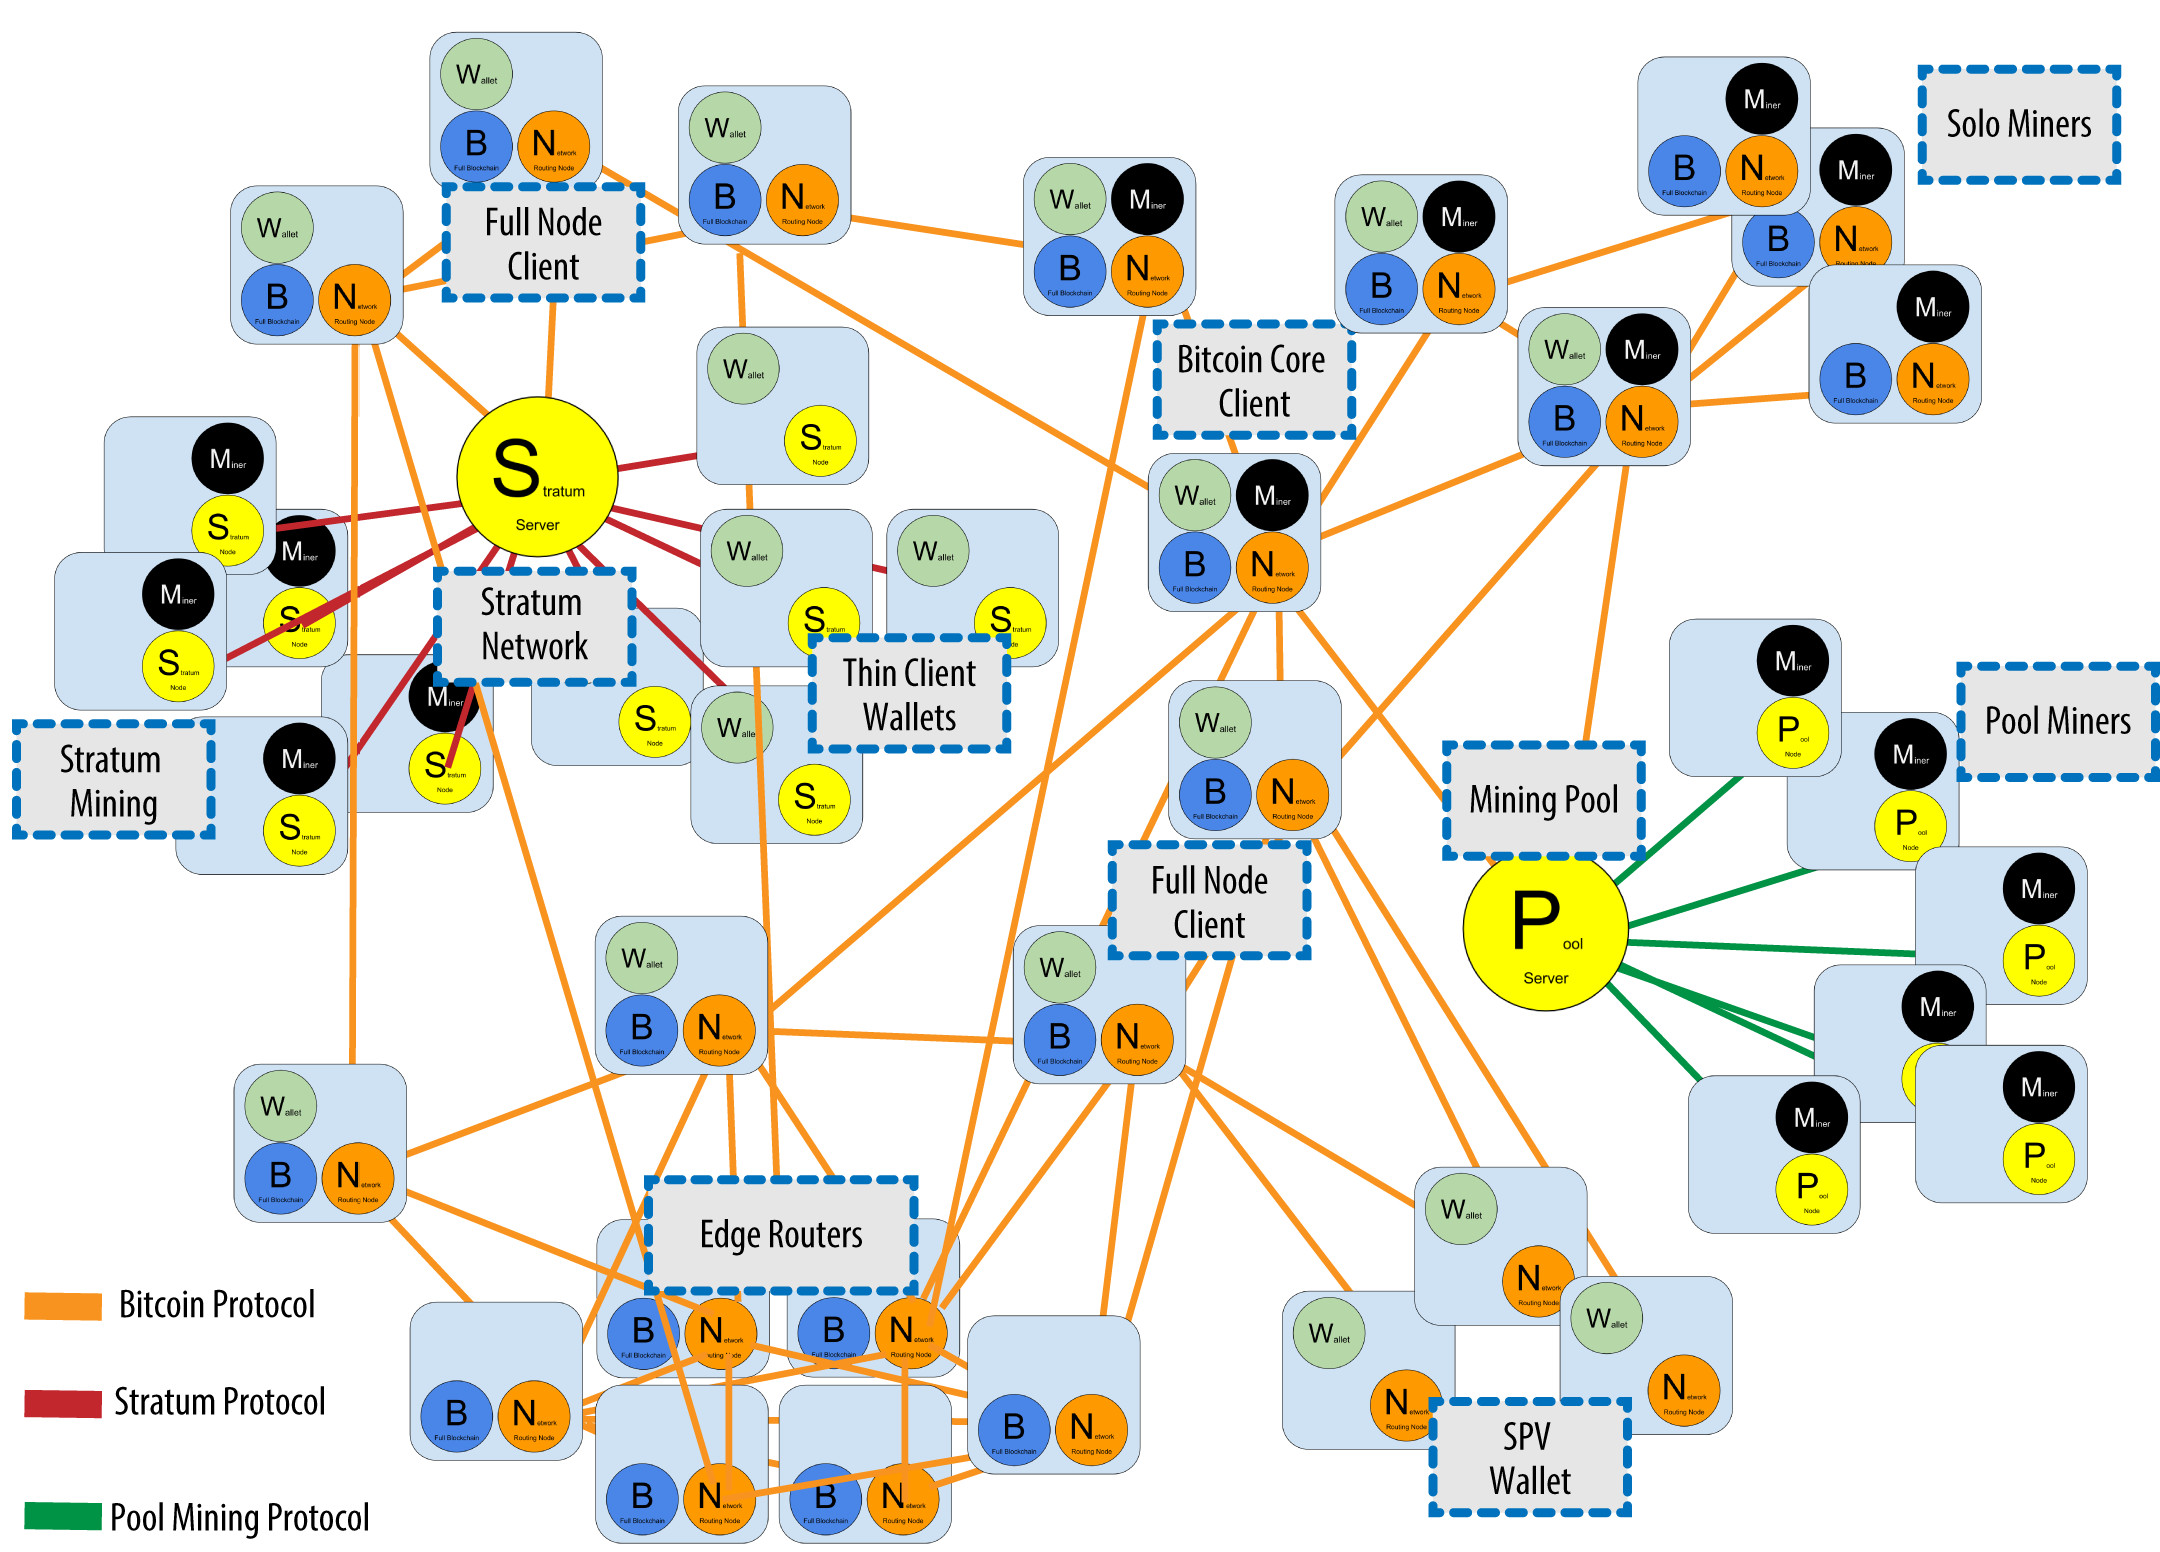
\includegraphics[width=1\columnwidth]{network-bitcoin} 
	\caption[Network bitcoin]{Rete estesa di bitcoin con vari tipologie di nodi, gateway e protocolli.}
	\label{fig:network-bitcoin} 
\end{figure}

\section{Blockchain}
La struttura dati blockchain risulta un'ordinata lista di blocchi contenenti transazioni back-linked\footnote{blocchi sono collegati a ritroso, ognuno si riferisce al blocco precedente presente nella catena}. La blockchain è spesso visualizzata come una pila verticale, con blocchi stratificati l’uno sopra l’altro e il primo blocco serve da fondamenta della pila. La visualizzazione dei blocchi impilati uno sopra l’altro provoca l’uso di terminologie come "altezza" (height) per riferirsi alla distanza dal primo blocco, e \textit{top} per riferirsi al blocco aggiunto più recentemente. Anche se un blocco ha solo un genitore, può temporaneamente avere multipli figli. Ognuno dei figli si riferisce allo stesso blocco del padre e contiene lo stesso hash (padre) nel campo \textit{previous block hash}. Multipli figli emergono durante un fork della blockchain, una situazione temporanea che accade quando differenti blocchi sono scoperti quasi simultaneamente da miner differenti. In questo caso solo un blocco figlio diventa parte della blockchain i il fork viene quindi risolto. Il campo \textit{previous block hash} risulta molto importante al fine di rendere le transazioni passate sempre più affidabili, tale campo infatti è incluso nell'header del blocco e per questo motivo influenza l'hash del blocco attuale. La modifica di una transazione all'interno di un blocco genitore porta alla modifica del proprio hash che di conseguenza porta alla modifica dell'hash figlio, questo fino al vertice della blockchain. Visto che per questo ricalcolo servirebbe un’enorme
potenza computazionale, l’esistenza di una lunga catena di blocchi fa si che la storia più profonda della blockchain sia immutabile, che è uno degli elementi chiave della sicurezza di bitcoin.
\begin{table}[]
	\centering
	\begin{tabular}{|c|c|p{6cm}|}
		\hline
		\textbf{Dim.} 		&	\textbf{Campo} 					& \textbf{Descrizione} \\ \hline
		4 byte						& Versione 							& Un numero di versione per tracciare upgrade al software e/o al protocollo \\ \hline
		32 byte 					& Hash del Blocco Precedente 		& Un riferimento all’hash del blocco precedente \\ \hline
		32 byte 					& Merkle Root 						& Un’hash della radice del merkle tree delle transazioni di questo blocco \\ \hline
		4 byte 						& Timestamp 						& Il tempo approssimato della creazione del blocco corrente (Unix Epoch)\\ \hline
		4 bytes 					& Target di Difficoltà				& Taghet di difficoltà dell’algoritmo di proof-of-work per questo blocco \\ \hline
		4 byte 						& Nonce 							& Un contatore utilizzato per l’algoritmo di proof-of-work\\ \hline
	\end{tabular}
	\caption{La struttura di un block header}
	\label{tab:struttura-block-header}
\end{table}
Nella Tabella \ref{tab:struttura-block-header} troviamo indicato anche \textit{Markle Root}, conosciuto anche come un \textit{binary hash tree}, è una struttura dati usata per indicizzare efficientemente e verificare l’integrità di un grande gruppo di dati. Sono usati in bitcoin per indicizzare tutte le transazioni in un blocco, producendo in sostanza un’impronta digitale dell’intero set di transazioni, provvedendo ad un efficiente processo di verifica se una transazione è inclusa nel blocco. 

\subsubsection{Target di difficoltà}
Il target determina la difficoltà e quindi influenza il tempo necessario per trovare una soluzione da parte dell'algoritmo \textit{proof-of-work}. Come sappiamo i bitcoin vengono generati ogni 10 minuti circa questo è il battito di emissione della valuta che deve rimanere costante negli anni. Col passare degli anni si avrà un rapido aumento della potenza di calcolo degli elaboratori e inoltre sempre più utenti prenderanno parte alla network bitcoin. Questo comporta che sarà sempre più facile arrivare ad una soluzione proof-of-work, perciò si deve procedere con l'aumento della difficoltà di tale algoritmo al fine di mantenere la generazione di nuovi blocchi fissa a 10 minuti. Questo retargeting avviene in modo automatico su ogni nodo. Ogni 2016 blocchi, tutti i nodi ritarano la difficoltà proof-of-work. L'equazione è semplice, si misura il tempo effettivo impiegato per generare gli ultimo 2016 blocchi e lo si confronta con il tempo atteso di 20160 minuti. 
\[ \text{New Difficulty = Old Difficulty * (Tempo degli ultimi 2016 Blocchi / 20160 min)} \]

\subsection{Fork della blockchain}
La blockchain è una struttura dati decentralizzata e le diverse copie nella network non sono sempre identiche. Come sappiamo la procedura di mining è una competizione globale nel tentativo di arrivare prima ad una soluzione proof-of-work- La velocità con cui l'aggiornamento della blockchain si propaga nella neetwork può far si che in caso due miner trovino due proof-of-work diverse, ma comunque valide, generano all'interno della rete un fork. Questo significa che il penultimo blocco aggiunto ha generato due o più figli. Da questo momento la network bitcoin si divide in sezioni, ognuna lavorerà per cercare di aggiungere un blocco al di sopra del blocco figlio che arrivò per primo. Con molta probabilità un solo altro miner troverà una soluzione che accrescerà una delle due ramificazioni. Da questo momento in poi la blockchain valida per tutti i miner sarà quella con proof-of-work più alto, la catena più lunga. L'effetto di questa scelta andrà ad incidere sul lavoro che altri miner hanno svolto sull'altro ramo della catena. Le transazioni incluse nei blocchi di quel ramo verranno scartate, tranne quelle non incluse nei blocchi dell'attuale catena principale, che verranno rimessi in coda. Un classico fork può capitare ogni settimana ma normalmente vengono risolte dopo il calcolo di un blocco, raramente due miner trovano altre due soluzioni quasi contemporaneamente. La visione grafica degli eventi appena descritti si possono vedere in Figura \ref{fig:fork-blockchain}.
\begin{figure}
	\centering
	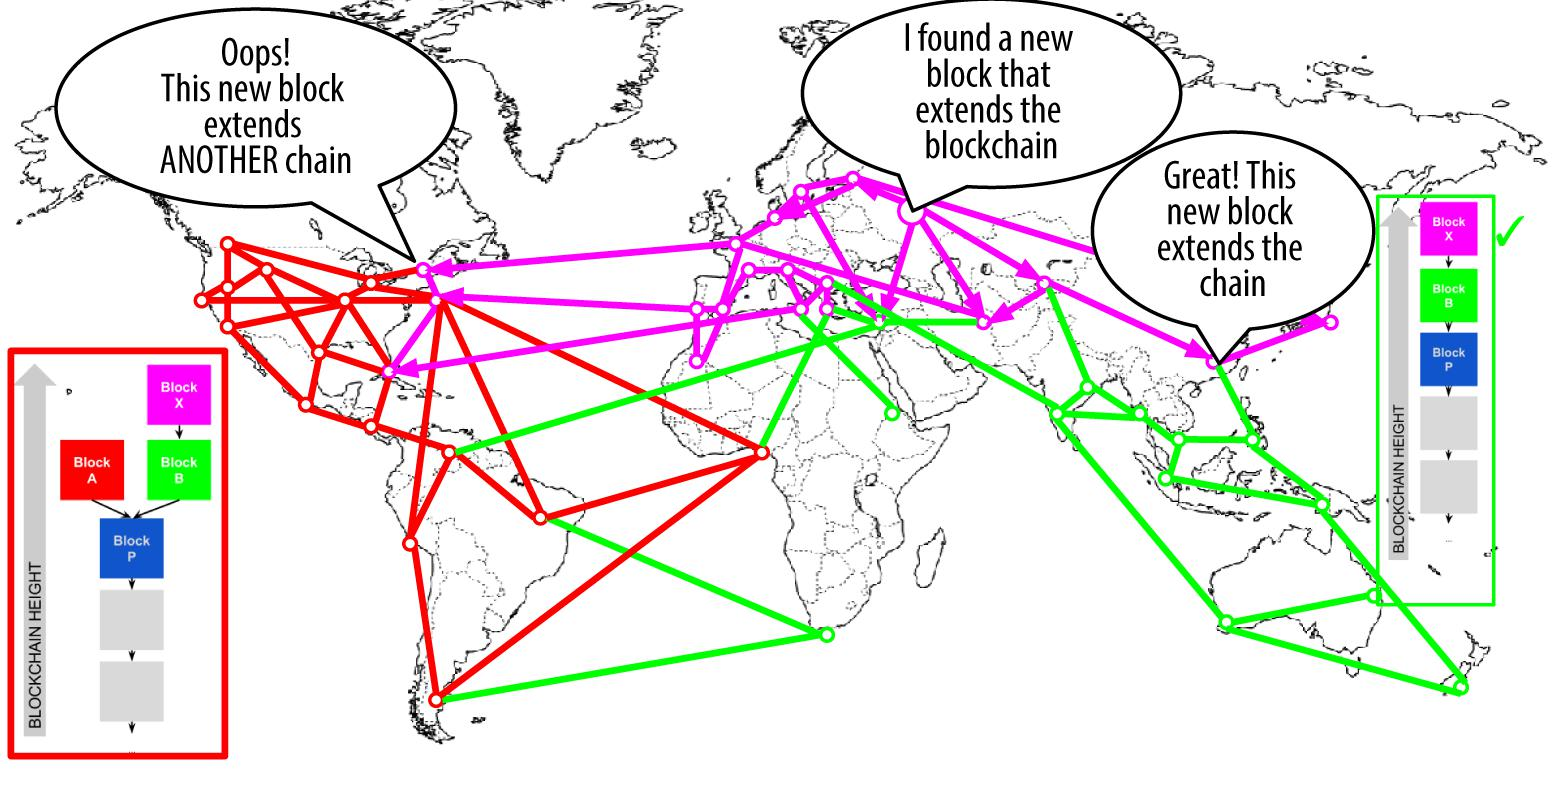
\includegraphics[width=1\linewidth]{Immagini/fork-blockchain}
	\caption[Visualizzazione di un’evento di fork di blockchain]{Visualizzazione di un’evento di fork di blockchain: il network riconverge su di una nuova longest chain}
	\label{fig:fork-blockchain}
\end{figure}

\subsection{Attacchi al consenso}
Il meccanismo di consenso in bitcoin dipende dal fatto che la maggioranza dei miner agisca onestamente, tuttavia se un miner o un gruppo di miner raggiunge una quota significativa del potere di calcolo, essi possono attaccare il meccanismo di consenso in modo da interrompere la sicurezza e la disponibilità della rete bitcoin. Gli attacchi di consenso possono influenzare il futuro e il passato più recente (all'incirca 10 blocchi), andando a forzare eventuali fork secondari della blockchain. Un fork può essere raggiunto da qualsiasi profondità ma nella pratica la potenza di calcolo necessaria per forzare un fork molto profondo risulta essere immensa. Questo rende i blocchi, confermati $n$ volte, praticamente immutabili. Un attacco di questo tipo non può spendere bitcoin senza l'utilizzo di firme, reindirizzare bitcoin o modificare in qualsiasi altro modo le transazioni. Gli attacchi di consenso possono interessare solo i blocchi più recenti e causare denial-of-service sulla creazione di blocchi futuri. Un attacco di questo tipo viene chiamato \textbf{Attacco del 51\%}, in questo scenario un gruppo di miner, controllando il 51\% della potenza di hashing della network bitcoin, hanno la possibilità di portare a termine con successo questo tipo di attacco. Possono causare deliberatamente dei fork, double-spending o eseguire attacchi di denial-of-service contro specifiche transazioni / indirizzi. Nonostante il suo nome, questo tipo di attacco in realtà non richiede il 51\% della potenza di hashing. Tale soglia rappresenta semplicemente il livello al quale l'attacco è quasi sicuramente di successo. Vari gruppi di ricerca, utilizzando degli strumenti statistici, affermano che vari tipi di attacchi di consenso sono possibili utilizzando anche solo il 30\% della potenza di hashing.

\section{Alt-Chain e Alt-Coin}
Bitcoin è il risultato di ben 20 anni di ricerca sui sistemi distribuiti e valute che ha portato ad una tecnologia rivoluzionaria: il meccanismo di consenso decentralizzato basato sulla proof-of-work. Questa invenzione è il cuore di bitcoin e ha successivamente generato un'onda di innovazione in valuta, servizi finanziari, eco	nomia, sistemi distribuiti, sistemi di votazione e contratti. Sono infatti nate delle:
\begin{description}
	\item[Alt-coin] valute digitali implementate utilizzando lo stesso modello di implementazione di bitcoin, la maggior parte delle implementazioni derivano da codice sorgente di bitcoin. Questo tipo di valuta sono chiamate anche \textit{fork} di bitcoin. Poi co sono anche delle alt-coin implementate da zero basate solamente sul modello blockchain ma che non riutilizzano il codice sorgente di bitcoin. Tra le principali troviamo Litecoin, Dogecoin, Freicoin, NXT.
	\item[Alt-chain] blockchain alternative il cui vero scopo non è quello di realizzare un sistema monetario. Queste diverse implementazioni possono comunque includere anche una valuta ma questa viene emessa come token per allocare dell'altro, come una risorsa o un contratto. Tra la principali troviamo Namecoin ed Ethereum.
\end{description}
% !TEX encoding = UTF-8
% !TEX TS-program = pdflatex
% !TEX root = ../Tesi.tex
% !TEX spellcheck = it-IT

%************************************************
\chapter{Ethereum}
\label{bitcoin-chapter}
%************************************************
In questo capitolo andremo ad approfondire Ethereum, una delle alt-chain in circolazione dopo la comparsa di bitcoin. Ethereum è una piattaforma che processa ed esegue smart contract Turing-completi basandosi su di un libro mastro blockchain. Non è un clone di Bitcoin ma bensì una nuova implementazione dal design completamente indipendente. Anche se, come alt-chain, non è tenuto ad esserne provvisto, Ethereum ha una propria moneta integrata, chiamata \textit{ether}, richiesta per pagare l'esecuzione di un contratto. La blockchain Ethereum registra i vari contratti che sono espressi in un linguaggio Turing-completo di basso livello. Uno smart contract è sostanzialmente un programma che gira su ogni nodo del sistema Ethereum. Tali contratti possono memorizzare dati, inviare / ricevere pagamenti in ether, memorizzare ether, ed eseguire una gamma infinita di azioni calcolabili, agendo come agenti decentralizzati di software autonomo.

\section{Introduzione}
Ethereum è spesso descritto come "the world computer". Dal punto di vista informatico Ethereum è una macchina a stati deterministica ma praticamente illimitata, costituita da uno stato sigleton accessibile a livello mondiale ed una propria macchina virtuale \textit{EVM} che applica le modifiche a tale stato. E' un'infrastruttura open source, globalmente decentralizzata sviluppata per eseguire programmi denominati \textit{smart contract}. Utilizza la blockchain per sincronizzare e memorizzare le modifiche di stato del sistema, assieme ad una criptovaluta chiamata \textit{ether} utilizzata per limitare le risorse per l'esecuzione dei contratti. 

Diversamente da Bitcoin, che ha un linguaggio di scriptiong molto limitato, Ethereum è stato concepito per essere una blockchain programmabile per l'uso generico che esegue una macchina virtuale in grado di eseguire codice di complessità arbitraria ed illimitata. Il linguaggio script di Bitcoin è stato intenzionalmente vincolato a delle semplici valutazioni true / false delle condizioni di spesa, il linguaggio di Ethereum invece risulta Turing-completo, può infatti funzionare come un general-purpose computer.

\subsection*{La nascita di Ethereum}
Ethereum è stato concepito in un momento in cui le persone hanno riconosciuto la potenza di un modello quale Bitcoin e stavano cercando di andare oltre alle applicazioni di criptovaluta. L'enigma principale era: costruire su Bitcoin o avveriare una nuova blockchin? Costruire al di sopra di Bitcoin significava vivere entro gli intenzionali limiti imposti da tale rete cercando soluzioni alternative. L'insieme limitato di tipologia di dati e dimensione della memorizzazione di questi sembrava limitare il numero di applicazioni che potevano essere eseguite su bitcoin, qualsiasi ulteriore aggiunta avrebbe implicato la nacessità di implementare ulteriori strati fuori catena, anullando così molti dei vantaggi nell'uso di una blockchain pubblica. Per tale progetto si necessitava di maggiore libertà e fluidità rimanendo on-chain, l'unica opzione era una nuova blockchain.

Verso la fine del 2013, Vitalik Buterin, un giovane programmatore apassionato di Bitcoin, pensò di estendere le capacità di Bitcoin e Mastercoin. Nell'ottobre di quell'anno, propose un approccio più generalizzato al team di Mastercoin, che consentiva contratti flessibili e programmabili, anche se non Turing-completi, in sostituzione dell'allora attuale linguaggio contrattuale di Mastercoin, ma questa proposta risultava una modifica troppo radicale er adattarsi alla loro roadmap di sviluppo. 

Nel dicembre 2013, Vitalik condivise un white paper che delineava l'idea di Ethereum: una blockchain Turing-completa per tutti gli usi. Si aggiunse al team  il Dr. Gavin Wood, attuale CTO, che lo aiutò nel perfezionale il protocollo che attualmente porta il nome di Ethereum. 

Lo sviluppo di Ethereum è stato pianificato in quattro fasi distinte, con importanti cambiamenti in ciascuna fase. Ogni fase può includere delle subreleases, note come "hard fork", che apportando funzionalità non retro compatibili. Le quattro fasi di sviluppo portano il nome di \textit{Frontier, Homestead, Metropolis, Serenity}. I fork intermedi programmati sono \textit{Ice Age, DAO, Tangerine Whistle, Spurious Dragon, Byzantinum e Costantinople}. Ma vediamoli in timeline:
\begin{description}
	\item[Blocco \#0] Frontier - Fase iniziale di Ethereum, 30 luglio 2015 - marzo 2016.
	\item[Blocco \#200000] Ice Age - Hard fork per introdurre un aumento di difficoltà esponenziale, per motivare la futura transazione verso PoS.
	\item[Blocco \#1150000] Homestead - Seconda fase di Ethereum lanciata a marzo 2016.
	\item[Blocco \#1192000] DAO - Hard fork che ha rimborsato le vittime del contratto DAO hacked causando la separazione di Ethereum ed Ethereum Classic.
	\item[Blocco \#2463000] Tangerine Whistle - Hard fork per modificare il calcolo del gas per certa operazioni di I/O.
	\item[Blocco \#2675000] Spurious Dragon - Hard fork per sventare vettori d'attacco DoS e meccanismi di protezione ai replay attack.
	\item[Blocco \#4370000] Metropolis Byzantium - Terza tappa di Ethereum lanciata nell'ottobre 2017
\end{description}
Dopo Byzantium, rimangono altri due hard fork Metropolis Costantinople ed a seguire la fase finale Serenity.

\subsection{Turing-completezza di Ethereum}
La capacità di Ethereum di eseguire un programma memorizzato, in un macchina a stati chiamata Ethereum Virtual Machine, mentre legge e scrive dati in memoria lo rende un sistema Turing Completo. Ethereum può infatti calcolare qualsiasi algoritmo che possa essere calcolato da qualunque macchina di Turing.
L'innovativa invenzione di Ethereum consiste nel combinare l'architettura di calcolo generica di un computer con l'affiancamento di una blockchai decentralizzata che memorizza il programma da eseguire. In questo modo si crea un computer mondiale distribuito (singleton). I programmi Ethereum funzionano ovunque producendo uno stato comune che viene garantito dalle regole di consenso. 
Il fatto che Ethereum si turing completo porta con se una conseguente problematica, il fatto che possa eseguire qualsiasi programma, di qualsiasi complessità. Questa flessibilità porta alcuni problemi dal punto di vista della sicurezza e di gestione delle risorse disponibili. 
Turing ha dimostrato che non è possibile prevedere se un programma terminerà o meno senza eseguirlo. Ciò pone una sfida: ogni nodo partecipante (client) dovrà convalidare ogni singola transazione, convalidando qualsiasi smart contract che chiama, ma come dimostrato da Turing, Ethereum non potrà sapere a priori se uno smart contract terminerà, o per quanto tempo verrà eseguito, senza effettivamente eseguirlo. Se per caso o di proposito fosse possibile creare un contratto facendo in modo che funzioni per sempre quando un nodo tenterà di convalidarlo si verificherebbe un attacco di tipo DoS. Per evitare che questo accada Ethereum introduce un meccanismo di misurazione delle risorse chiamato \textit{gas}. Quando l'EVM esegue uno smart contract tiene accuratamente conto di ogni istruzione (calcolo, accesso ai dati, ecc \dots). Ogni istruzione ha un proprio costo predeterminato in \textit{gas}. Quando una transazione attiva l'esecuzione di un contratto, deve includere una quantità di \textit{gas} che imposta come limite superiore di ciò che può essere consumato eseguendo tale smart contract. Le unità di gas devono essere incluse quindi acquistate con l'ether, durante il calcolo della transazione.

\subsection{Dalla Blockchain generica alle \DH Apps}
Ethereum è nato con l'intenzione di creare una blockchain general-purpose che potesse essere programmata per svariati usi. Molto rapidamente la visione di Ethereum si è espansa fino a diventare una piattaforma per programmare DApps. Queste DApps presentano una prospettiva più ampia rispetto agli smart contract. Una DApp è come minimo un contratto munito però di un'interfaccia web utente. Più in generale, una DApp è un'applicazione Web costruita su servizi di un'infrastruttura aperta, decentralizzata e peer-to-peer. Lo si può anche trovare scritto in questo modo \DH App. Il carattere \DH rappresenta il carattere latino \textit{ETH} che appunto allude a Ethereum.

\subsection{Le unità monetarie di Ethereum}
L'unità monetaria di Ethereum si chiama \textit{ether} ed è identificata con il nome di \textit{ETH}. Un ether è suddiviso in unità più piccole, fino all'unità più piccola chiamata \textit{wei}. All'interno di Ethereum il valore di \textit{ether} viene sempre rappresentato in \textit{wei}. Le denominazioni delle varie frazioni di ether hanno sia un nome scientifico che utilizza il sistema internazionale di unità, SI, sia un nome colloquiale che rende omaggio a molte delle più grandi menti della matematica e della crittografia, tutte le denominazioni sono riportate in Tabella \ref{tab:frazioni-di-ether}.
\begin{table}[]
	\centering
	\begin{tabular}{|l|c|c|c|}
		\hline
		\textbf{Valore (in wei)}			& \textbf{Esp.}	& \textbf{Nome} & \textbf{Nome \textit{SI}}\\ \hline
		1 									&	$1$			&	wei			&	Wei\\ \hline
		1.000 								&	$10^{3}$	&	Babbage		&	Kilowei o femtoether\\ \hline
		1.000.000 							&	$10^{6}$	&	Lovelace	&	Megawei o picoether\\ \hline
		1,000,000,000						&	$10^{9}$	&	Shannon		&	Gigawei o nanoether\\ \hline
		1.000.000.000.000					&	$10^{12}$	&	Szabo		&	Microetere o micro\\ \hline
		1.000.000.000.000.000				&	$10^{15}$	&	Finney		&	Milliether o milli\\ \hline
		1.000.000.000.000.000.000			&	$10^{18}$	&	Ether		&	Ether\\ \hline
		1.000.000.000.000.000.000.000		&	$10^{21}$	&	Grand		&	Kiloether \\ \hline
		1.000.000.000.000.000.000.000.000	&	$10^{24}$	&				&	Megaether \\ \hline
	\end{tabular}
	\caption{Denominazioni delle frazioni di ether.}
	\label{tab:frazioni-di-ether}
\end{table}

\subsection*{Wallet}
Il termine wallet rappresenta tutti quei software che aiutano l'utente nella gestione del proprio account Ethereum, memorizza infatti le chiavi d'accesso ai fondi, crea e trasmette transazioni. Esistono varie tipologie di wallet, che richiedono più o meno attenzione per la gestione delle chiavi, più controllo e indipendenza si vuole avere, più aumentano le responsabilità. Un buon wallet è per esempio MetaMask, portafoglio web-based che si presenta come un'estensione per i browser più comuni come Chrome, Firefox e Opera. Risulta facile da usare e conveniente per eseguire test, poichè risulta in grado di connettersi ad una vasta gamma di nodi Ethereum per testare la blockchain. L'installazione di MetaMask risulta veramente semplice, infatti basterà aprire il gestore estensioni del proprio browser e cercare tale estensione e una volta individuata procedere con l'istallazione. Al termine della procedura si aprirà automaticamente la schermata principale di MetaMask dove ci viene richiesto di inserire una password. Tale password servirà per impedire a chiunque utilizzi il computer in questione e quindi ha accesso al browser su cui è installato MetaMask, di accedere a tale wallet e quindi aver accesso ai fondi. A questo punto viene generato un backup mnemonico formato da 12 parole inglesi. Queste parole potranno essere utilizzate in qualsiasi wallet compatibile per recuperare l'accesso al proprio conto in caso di guasti di qualsiasi tipo. Si consiglia di conservare un backup cartaceo delle credenziali d'accesso e del backup mnemonico riponendolo in un luogo fisicamente sicuro. Si sconsiglia infatti di salvare digitalmente tali informazioni.
A questo punto ci troveremo davanti ad una schermata dove ci viene mostrato il nostro conto. Troviamo varie informazioni tipo il nostro indirizzo casualmente generato, il saldo del conto, lo storico delle transazioni passate e in corso. In questa schermata sarà anche possibile selezionare la rete sulla quale inviare le nostre transazioni. Le varie reti disponibili sono:
\begin{itemize}
	\item \textbf{Rete principale di Ethereum:} principale blockchain pubblica di Ethereum, in questa rete il valore in ether è reale e ogni azione avrà conseguenze reali.
	\item \textbf{Rete di test Ropsten:} rete con blockchain pubblica in cui ether non ha valore.
	\item \textbf{Rete di test Kovan:} rete con blockchain pubblica in cui ether non ha valore. Utilizza il protocollo di consenso Aura. Questa rete è supportata solo da Parity, gli altri client il protocollo di consenso Clique, proposto in seguito. 
	\item \textbf{Rete di test Rinkeby:} rete con blockchain pubblica, utilizza il protocollo di consenso Clique. Anche in questa rete Ether non ha valore.
	\item \textbf{Localhost 8545:} Si connette ad un nodo in esecuzione sullo stesso computer del browser. Tale noto può far parte di una blockchain pubblica o di una rete di test privata.
	\item \textbf{RPC personalizzata:} consente di collegare MetaMask a qualsiasi nodo con un'interfaccia \textit{RPC} (Remote Procedure Call) compatibile con Geth. Tale nodo può essere parte di una blockchain pubblica o privata. 	
\end{itemize}
Prenderemo come esempio la \textit{rete di test Ropsten}.

Per muovere i primi passi su Ethereum, o qualsiasi altra blockchain, abbiamo bisogno di fondi. Per eseguire dei test possiamo richiedere dei fondi gratuitamente sulle reti di test, per esempio Ropsten. Quindi da MetaMask selezioniamo la sopracitata rete di test selezioniamo \textit{Deposita > Ottieni Ether}, a questo punto si aprirà un'altra scheda dove poter richiedere \textit{1 ether from faucet}. Una volta eseguita la richiesta, in basso, nella sezione \textit{transactions} comparirà l'ID della transazione appena eseguita per trasferire 1 ether sul nostro conto. Attendendo qualche secondo la somma richiesta vi verrà accredita e possiamo effettuare dei pagamenti. Per fare ciò dobbiamo tenere conto del \textit{gas}, commissione raccolta dai minatori per convalidare la transazione. Il costo massimo corrisponde a :
\[ 3*21000 \text{ gwei} \quad = \quad 63000 \text{ gwei} \quad = \quad 0.000063 \text{ ETH}\]
Questo sta a significare che una transazione di $ 1 \text{ ETH} $ costerà $ 1.000063 \text{ ETH} $, nonostante MetaMask visualizzi cifre approssimate, omettendo di visualizzare le cifre meno significative, sia nel saldo del conto che nel totale delle singole transazioni.

Durante la presentazione di Ethereum abbiamo anticipato che una delle particolarità di questa nuova blockchain sta proprio nella possibilità implementazione di smart contract da sottomettere al computer mondiale Ethereum. Vediamo ora come creare il primo contratto che ci darà la possibilità di depositare ether sul conto del contratto creato e successivamente procedere con il prelievo di massimo 0.1 ether. Il contratto che andremo a creare si chiama \textit{faucet} e verrà scritto in Solidity tramite Remix\footnote{Remix è un IDE per la scrittura di Smart Contract in linguaggio Solidity, tramite browser. http://remix.ethereum.org}. Il funzionamento di questo contratto è semplice: distribuisce ether a qualsiasi indirizzo che ne richiede e il conto di tale contratto può essere caricato periodicamente. Per procedere quindi dobbiamo copiare il codice qui riportato all'interno di un nuovo file \textit{faucet.sol} all'interno di Remix. A questo punto l'IDE compilerà in automatico mostrando un riquadro verde riportante il nome del contratto. Ora siamo pronti per inviare questo smart contract sulla blockchain pubblica e successivamente testarlo.
\begin{lstlisting}
// Our first contract is a faucet!
pragma solidity ^0.4.19;

contract Faucet {
   // Give out ether to anyone who asks
   function withdraw(uint withdraw_amount) public {
      // Limit withdrawal amount
      require(withdraw_amount <= 100000000000000000);	■\label{line:max_amount}■
      // Send the amount to the address that requested it
      msg.sender.transfer(withdraw_amount);
   }
   // Accept any incoming amount
   function () public payable {}
}
\end{lstlisting}
La registrazione di un contratto sulla blockchain comporta la creazione di una transazione speciale la cui destinazione è l'indirizzo $0\text{x}000 \dots 000$ noto come indirizzo zero, facendo capire alla blockchain Ethereum che siamo intenzionati a registrare un nuovo smart contract. Fortunatamente Remix riesce ad interagire con MetaMask, semplicemente impostando la voce in \textit{Run > Environment} sul valore \textit{Injected Web3 - Ropsten}. Subito al di sotto di questa voce troviamo la voce \textit{Deploy} che procederà con la creazione di una nuova transazione che portando alla registrazione del contratto. Una volta confermata tale transazione possiamo richiamare la funzione \textit{withdraw(uint withdraw\_amount)} inserendo massimo 0.1 ETH, limite impostato alla riga \ref{line:max_amount}, nell'apposito campo della scheda Run, vista in precedenza e procedere premendo il pulsante \textit{transact}. A questo punto verrà creata una nuova transazione verso l'indirizzo del contratto richiedendo tale somma di ether. Se tutto andrà a buon fine, il contratto esaminerà tale richiesta e produrrà un'ulteriore transazione trasferendo la cifra indicata verso il nostro conto. Si consiglia di utilizzare https://ropsten.etherscan.io per visualizzare tutti i dettagli delle varie transazioni, una cosa importante da notare è il fatto che le transazioni di risposta di contratti non vengono riportate nel tab \textit{Transaction}, ma compariranno nel tab \textit{Internal Txns}.

\section{Le transazioni}
Le transazioni sono messaggi firmati originati da un account di proprietà che vengono trasmessi della rete Ethereum e registrati sulla blockchain. La struttura di base di una transazione è quella che vediano in tabella \ref{tab:struttura_base_transazioni}.
%
\begin{table}[]
	\centering
	\begin{tabular}{|c|p{11cm}|}
		\hline
		\textbf{Campo} & \textbf{Descrizione} \\ \hline
		nonce & Numero di sequenza emesso dall'EOA di origine, utilizzato per impedire il replay attack.\\ \hline
		gas price & Prezzo del gas in wei che il mittente è disposto a pagare.\\ \hline
		gas limit & Quantità massima di gas che l'EOA di origine è disposto ad acquistare per la transazione corrente.\\ \hline
		recipient & Indirizzo Ethereum a cui è destinata la transazione. \\ \hline
		value & Quantità di ether da inviare a destinazione.\\ \hline
		data & Lunghezza variabile del payload.\\ \hline
		v, r, s & Tre componenti della firma digitale ECDSA dell'EOA di origine.\\ \hline
	\end{tabular}
	\caption{Struttura base di una transazione Ethereum.}
	\label{tab:struttura_base_transazioni}
\end{table}
%
La struttura del messaggio transazione viene serializzata utilizzando lo schema di codifica RLP (Recursive Length Prefix), creato appositamente per semplificare la serializzazione dei dati in Ethereum. Tutti i numeri vengono codificati come interi big-endian, di lunghezze che sono multipli di 8 bit. Le etichette di campo non fanno parte dei dati serializzati della transazione, che contiene valori di campo codificati in RLP. In generale RLP non contiene alcun delimitatore o etichetta di campo e la lunghezza di ciascun campo viene identificata tramite un prefisso. Molte informazioni visualizzate da wallet e altri strumenti sono derivate da altre più primitive. Per esempio la chiave pubblica dell'EOA può essere ricavata dalle componenti \textit{v, r, s} della firma ECDSA.

\subsection*{Nonce}
Il nonce è uno dei componenti più importanti ma meno comprese in Ethereum. La definizione che troviamo nel White Paper si legge: \textit{"nonce: numero scalare uguale al numero di transazioni inviate da questo indirizzo, o nel caso di account con codice associato, il numero di creazioni di contratto effettuate da questo account"}. Esistono due scenari in cui l'esistenza di un nonce risulta importane.
\begin{enumerate}
	\item Supponiamo di aver due transazioni da effettuare, una puù importante dell'altra ma non disponiamo di un saldo sufficiente per pagare entrambe le transazioni. Se inviassimo, in un sistema decentralizzato come Ethereum, prima la transazione più importente e poi la seconda, non disponendo del campo nonce, non abbiamo la certezza che la prima transazione venga sicuramente eseguita prima dell'altra, dato che i nodi possono ricevere le transazioni in entrambi gli ordini.
	\item Immaginiamo ora di possedere un portafoglio Ethereum con parecchi fondi, e di fare un trasferimento di pochi ether ad un altro indirizzo. Senza il campo nonce un qualsiasi altro untente che vede tale transazione la potrà replicare fintanto chè sul nostro conto abbiamo fondi a sufficienza da coprire la cifra versata.
\end{enumerate}
Il campo nonce ha un duplice scopo, dare un ordine di esecuzione alle transazioni, sostanzialmente l'ordine di creazione, ed essendo unico, serve a sventare i replay attack.

\subsection{Gas di transazione}
Come abbiamo già detto precedentemente, il gas è il carburante di Ethereum, una valuta virtuale separata da l'ether con il proprio tasso di cambio. Ethereum utilizza il gas per controllare la quantità di risorse che una transazione può utilizzare dal momento che il modello di calcolo a terminazione aperta (Turing completo) richiede una qualche forma di misurazione al fine di evitare attacchi di denial-of-service. Il gas è separato dall'ether per proteggere il sistema dalla volatilità che potrebbe insorgere assieme ai rapidi cambiamenti nel valore dell'ether. Il cambio gas / ether può quindi variare al valiare del valore della valuta ether. 

Il campo getPrice in una transazione consente all'ordinante di impostare il prezzo che è disposto a pagare in cambio del gas. Il prezzo è misurato in wei per unità di gas. I wallet possono regolare il prezzo del gas nelle transazioni per ottenere una conferma più rapida, maggiore sarà il prezzo del gas, più rapida sarà la conferma della transazione. Il valore minimo a cui getPrice può essere impostato è zero. Queste transazioni risulteranno quindi completamente gratuite ma rischiano di non essere mai confermate. 

Se l'indirizzo di destinazione è uno smart contract, la quantità di gas può essere stimata ma non può essere determinata con precisione. Questo perchè un contratto può valutare diverse condizioni che portano a diversi percorsi di esecuzione, con conseguenti costi totali di gas diversi. 

\subsection*{Destinatario della transazione}
Il destinatario della transazione viene specificato nel campo \textit{to}. Questo contiene un indirizzo Ethereum di 20 byte che può essere un EOA o un indirizzo di un qualche contratto. Ethereum con convalida ulteriormente questo campo, qualsiasi valore di 20 byte è considerato valido. E' possibile inviare fondi ad un indirizzo che non ha alcuna chiave privata o contratto corrispondente, in questo modo gli ether inviati vengono persi e non saranno più spendibili. La convalida deve quindi essere eseguita a livello di interfaccia utente.

\subsection{Creazione contratti}
La creazione di un contratto implica la generazione di una transazione speciale per procedere alla distribuzione di tale contratto. Le transazioni che procedono alla registrazione di un contratto su blockchain vengono indirizzate verso uno speciale indirizzo chiamato indirizzo zero che non rappresenta né un EOA né un contratto. Viene infatti utilizzato come destinazione con un significato speciale: \textit{"crea questo contratto"}. Tuttavia questo indirizzo a volte riceve pagamenti da vari indirizzi, o per caso, con la conseguente perdita di ether, o per intenzionale volontà di rendere non spendibile una certa somma di ether.

Una transazione di creazione contratto deve contenere solo un payload di dati contenente il bytecode compilato che creerà il contratto. E' comunque possibile includere un importo di ether nel campo del valore se si desidera creare un contratto con un saldo iniziale pari a tale versamento, ma è del tutto facoltativo. Questa operazione può essere eseguita anche dopo la creazione del contratto, attendendo la fine di tale operazione, andando quindi a copiare l'indirizzo Ethereum di tale contratto e creando una nuova transazione che trasferirà un quantitativo di ether a questo indirizzo.

\subsection*{Firme digitali}
L'algoritmo di firma di Ethereum è l'Elliptic Curve Digital Signature (ECDSA) che si basa su coppie di chiavi pubbliche e private calcolate appunto su curve ellittiche. Lo scopo della firma digitale è risassunto nei seguenti punti:
\begin{enumerate}
	\item Dimostra che il proprietario della chiave privata, che implicitamente è anche il proprietario del conto Ethereum, ha autorizzato la spesa di ether o l'esecuzione di un contratto.
	\item Garantisce la non-repudiation: la prova di tale approvazione non è negabile.
	\item Dimostra che i dati della transazione non sono stati e non possono essere modificati da nessuno dopo che la transazione è stata firmata.
\end{enumerate}

\subsubsection{Creazione della Firma Digitale}
Ethereum, per attuare l'ECDSA, dovrà firmare un messaggio, che nel nostro caso è la transazione, o più precisamente l'hash Keccak-256 dei dati con codifica RLP. La chiave di firma è la chaive privata dell'EOA ed il risultato sarà:
%
\[ Sig = F_{sig}( F_{kacak256}(m), k )\]
%
\begin{table}[]
	\centering
	\begin{tabular}{|c|l||c|l|}
		\hline
		$k$ & Chiave Privata & $m$ & Transazione RLP-encoded \\ \hline
		$F_{kacak256}$ & Funzione hash Kecak-256 & $F_{sig}$ & Algoritmo di firma \\ \hline
	\end{tabular}
\caption{Descrizione dei campi della funzione sign.}
\label{tab:descr_fun_sign}
\end{table}
%
La funzione $F_{sig}$ produce così la firma $Sig$ che risulterà composta da due valori comunemente denominati con $r$ e $s$:
%
\[Sig = (r, s)\]
%
Questo algoritmo per calcolare questi due valori $r$ e $s$ ha generato una chiave privata temporanea in modo crittograficamente sicuro. Come sappiamo infatti la chiave privata temporanea viene utilizzata per derivare la chiave pubblica, quindi abbiamo:
\begin{itemize}
	\item Un numero casuale $q$ crittograficamente sicuro, utilizzato come chiave privata temportanea.
	\item La corrispondente chiave pubblica $Q$, generata da $q$ e il punto $G$ generatore della curva ellittica.
\end{itemize}
Il valore $r$ della firma digitale, è la coordinata x della chiave pubblica $Q$. Da lì, l'algoritmo calcolerà $s$ della firma in moto che:
%
\[ s \equiv q^{-1} ( Kecak256( m ) + r * k )( \text{mod } p ) \]
%
Qui troviamo riportati i significati dei vari simboli all'interno della formula:
\begin{table}[h]
	\centering
	\begin{tabular}{|c|l||c|l|}
		\hline
		$q$ & chiave privata temporanea & $r$ & coordinata x della chiave pubblica\\ \hline
		$m$ & dati della transazione & $p$ & ordine primo della curva ellittica\\ \hline
	\end{tabular}
\end{table}
%
La verifica di correttezza risulta essere l'inverso della funzione di firma, utilizzando i valori $r$, $s$, e la chiave pubblica del mittente si sarà in grado di calcolare un valore $Q$ che sarà il punto sulla curva ellittica. I passi sono i seguenti:
\begin{enumerate}
	\item Controllare che tutti gli input siano stati forniti correttamente;
	\item Calcolare $ w = s^{-1} \text{ mod }p $.
	\item Calcolare $ u_{1} = Kekak256( m ) * w \text{ mod } p $.
	\item Calcolare $ u_{2} = r * w \text{ mod } p $.
	\item Infine, calcolare il punto sulla curva ellittica $ Q \equiv u_{1} * G + u_{2} * K (\text{mod } p)$.
\end{enumerate}
Se la coordinata $x$ del punto appena calcolato $Q$ risulta uguale a $r$, allora il verificatore può concludere che la firma è valida. Si noti che per tale verifica, la chiave privata non è né conosciuta né rivelata.
Per produrre una transazione valida, il mittente deve firmare digitalmente il messaggio, utilizzando l'algoritmo di firma digitale a curva ellittica. Quando diciamo \textit{"firmare la transazione"} intendiamo effettivamente \textit{"firmare l'hash $Keccak-256$ dei dati della transazione serializzati su RLP"}. La firma viene quindi applicata all'hash, non alla transazione stessa. Per firmare  una transazione in Ethereum, il mittente deve:
\begin{enumerate}
	\item Creare una struttura dati di transazione, contenente nove campi: \textit{nonce, gasPrice, gasLimit, to, value, data, chainID, 0, 0}.
	\item Produrre un messaggio serializzato con codifica RLP della struttura dei dati della transazione.
	\item Calcolare l'hash $Keccak-256$ di questo messaggio serializzato.
	\item Calcolare la firma ECDSA, firmando l'hash con la chiave privata dell'EOA di origine.
	\item Aggiungere i valori calcolati $v$, $r$ e $s$ della firma ECDSA alla transazione.
\end{enumerate}
L'identificatore di ripristino $v$ viene utilizzato per indicare la parità della componente $y$ della chiave pubblica.
Le tre fasi creazione, firma e trasmissione di una transazione, normalmente vengono eseguite come una singola operazione. Tuttavia è possibile creare e firmare una transazione in due passaggi separati. Una volta che una transazione viene firmata è possibile inviarla sulla rete Ethereum in un secondo momento. La ragione più comune per eseguire ciò è la sicurezza. Infatti il computer che firma la transazione deve conoscere le chiavi private che per forza di cose si devono trovare in memoria. Il computer che esegue la trasmissione deve essere collegato ad Internet. Se queste due funzioni sono sulla stessa macchina, allora le chiavi private sono salvate su di un sistema online, il che è piuttosto pericoloso. Questa procedura di separazione viene chiamata firma offline ed è una pratica di sicurezza comune, uno schema di questa procedura è riportato in Figura \ref{fig:ofline_signing}. Il sistema con la sicurezza maggiore risulta il sistema di tipo air-gapped, in tale sistema non vi è alcuna connettività di rete tra il computer online, colui che trasmetterà, e il computer che firma tale messaggio. Per firmare le transazioni e trasferirle da e verso la macchina online saranno necessari dei dispositivi di supporto dati o una webcam con relativo QRCode. Questa tecnica, per quanto sicura non risulta scalabile, dal momento in cui ogni transazione va trasferita manualmente tra le macchine.
\begin{figure}
	\centering 
	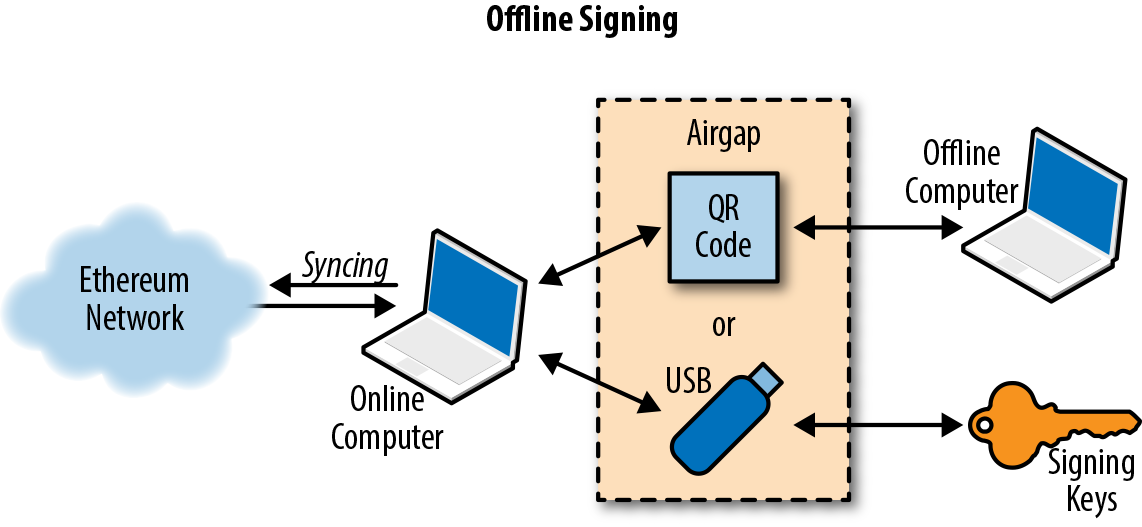
\includegraphics[width=1\columnwidth]{offline_signing} 
	\caption[Firma offline delle transazioni di Ethereum]{Firma offline delle transazioni di Ethereum}
	\label{fig:ofline_signing} 
\end{figure}

\section{Smart Contract}
Il termine smart contract è stato usato nel corso degli anni per descrivere un'ampia varietà di cose differenti. Nel contesto di Ethereum il termine in realtà è un po' improprio dato che gli smart contract Ethereum non sono né smart (intelligenti), né contract (legali). Tali contratti fanno piuttosto riferimento a programmi informatici immutabili che funzionano in modo deterministico in un contesto quale la macchina virtuale Ethereum (EVM) sul computer decentralizzato Ethereum. Ma vediamo questa affermazione per step:
\begin{description}
	\item[Programmi per computer] Gli smart contract sono semplicemente dei programmi per computer. La parola "contratto" non ha alcun significato legale per questo contesto.
	\item[Immutabile] Una volta implementato, il codice di un contratto non può essere cambiato, a differenza di un software tradizionale. Infatti l'unico modo per portare delle modifiche ad un proprio contatto è quello di ridistribuirne una nuova istanza.
	\item[Deterministico] L'esito di uno smart contract sarà lo stesso per tutti coloro che lo eseguiranno, dato il contesto della transazione e lo stato della blockchain Ethereum al momento di tale esecuzione.
	\item[Contesto EVM] Gli smart contract operano con un contesto di esecuzione limitato. Possono accedere al loro stato, al contesto della transazione che li ha richiamati e ad alcune informazioni sui blocchi più recenti.
	\item[Computer mondiale decentralizzato] L'EVM viene eseguita come istanza locale su ogni nodo Ethereum, ma poiché tutte le istanze di EVM operano sullo stesso stato iniziale e produrranno lo stesso stato finale, il sistema nel suo complesso opera come un singolo computer mondiale.
\end{description}
%
\subsection{Ciclo di vita di uno Smart Contract}
Gli smart contract sono solitamente scritti in un linguaggio di alto livello, come ad esempio Solidity. Per essere eseguiti nella EVM devono poi essere compilati in bytecode. Una volta compilati possono essere distribuiti sulla piattaforma Ethereum tramite la speciale transazione di creazione contratto che invia tale transazione all'indirizzo 0x0. Ogni contratto è identificato da un proprio indirizzo Ethereum che può essere utilizzato per l'invio di fondi o per richiamare le funzione in esso specificate. Diversamente dagli EOA, uno smart contract non ha associate delle chiavi. Tali contratti vengono eseguiti solamente se richiamati da una transazione. Un contratto può richiamare un altro contratto ma il primo della catena sarà per forza di cose richiamato da un qualche EOA. Nel caso in cui l'esecuzione dovesse fallire per un qualche motivo, termine gas o errore di qualche tipo, tutti i cambiamenti di stato avvenuti fino a quel momento vengono ripristinati a prima dell'esecuzione come se la transazione non fosse mai stata eseguita. Una transazione fallita viene comunque registrata come tentata, e l'etere speso a gas per l'esecuzione viene detratto dall'account di origine. 

Come accennato in precedenza, è importante ricordare che il codice di uno smart contract non può essere modificato. Tuttavia, un contratto può essere \textit{cancellato}, rimuovendo il codice e il suo stato interno, archiviazione, dal suo indirizzo, lasciando un account vuoto. Qualsiasi transazione inviata a quell'indirizzo dell'account dopo che il contratto è stato eliminato non comporta l'esecuzione di alcun codice, perché non esiste più alcun codice da eseguire. Per fare ciò si dovrà eseguire un apposito codice operativo chiamato SELFDESTRUCT. Tale operazione cosa una cifra in gas negativa, una sorta di rimborso del gas, questo per incentivare il rilascio di risorse. L'eliminazione di un contratto in questo modo non rimuove la cronologia delle transazioni del contratto, poiché la blockchain stessa è immutabile. La funzionalità SELFDESTRUCT sarà disponibile solamente se l'autore del contratto ha programmato il contratto per ottenere tale funzionalità, in caso contrario il contratto non potrà essere cancellato.

\subsection*{Linguaggi di alto livello per Ethereum}
L'EVM è una macchina virtuale che esegue una speciale forma di codice chiamata bytecode EVM, analoga alla CPU di un comune computer, che esegue codice macchina come x86\_64. E' possibile programmare i contratti Ethereum direttamente in bytecode, tuttavia la maggior parte dei programmatori preferisce ovviamente utilizzare un linguaggio di alto livello per poi convertire il codice prodotto in bytecode tramite un compilatore ad hoc. I linguaggi di programmazione possono essere classificati in due ampi paradigmi di programmazione: \textit{dichiarativo} e \textit{imperativo} , anche noti rispettivamente come \textit{funzionali} e \textit{procedurali}. Nella procedura dichiarativa, scriviamo funzioni che esprimono la logica di un programma, ma non il suo flusso. Viene utilizzata per creare programmi in cui non ci sono effetti collaterali, non ci saranno, infatti, combiamenti di stato al di fuori di una funzione. Haskel e SQL sono due di questi. Nella programmazione imperativa, al contrario, una procedura può cambiare sia la logica che il flusso di un programma. In questo contesto troviamo C++ e Java. Poi ci sono dei linguaggi di programmazione ibridi che incoraggiano la programmazione dichiarativa ma possono essere utilizzate anche per esprimere un paradigma di programmazione imperativo. Qui troviamo Lisp, JavaScript e Python. Qualsiasi linguaggio imperativo può essere usato per scrivere un paradigma dichiarativo. I linguaggi puramente dichiarativi, invece, non possono essere usati per scrivere un paradigma imperativo.

Mentre la programmazione imperativa è più comunemente utilizzata dai programmatori, può essere molto difficile scrivere programmi eseguiti esattamente come previsto. La capacità di qualsiasi parte del programma di cambiare lo stato di qualsiasi altro rende difficile ragionare sull'esecuzione di un programma e introduce molte opportunità per i bug. Nei contratti intelligenti, i bug costano letteralmente denaro e di conseguenza, è di fondamentale importanza scrivere contratti intelligenti senza effetti indesiderati. Per questo motivo, i linguaggi dichiarativi svolgono un ruolo molto più importante negli smart contract. Tuttavia, il linguaggio più utilizzato per i contratti intelligenti risulta Solidity che è imperativo.

\section{Solidity}
Solidity è stato creato dal Dr. Gavin Wood come linguaggio esplicito per scrivere smart contract per Ethereum. Il principale prodotto del progetto Solidity è il compilatore, \textit{solc}, che converte i programmi scritti in Solidity in linguaggio bytecode EVM. Ogni versione del compilatore corrisponde e compila una versione specifica di Solidity. Tale linguaggio segue un modello di versioning chiamato semantic versioning, che specifica la versione strutturandola in tre parti numeriche: MAJOR:MINOR:PATCH.

E' possibile installare il compilatore Solidity su Ubuntu / Debian seguendo le istruzioni riportate sull'apposita pagina http://olidity.readthedocs.io. Come già detto in precedenza ne esiste anche una versione web-based che include un IDE chiamato Remix, pensato per test iniziali e lo sviluppo di piccoli Smart Contract.

\subsection{Variabili e funzioni locali predefinite}
Quando un contratto viene eseguito nell'EVM, ha accesso ad un piccolo insieme di oggetti globali, tra cui \textit{block}, \textit{msg}, e \textit{tx}.
\begin{itemize}
	\item \textbf{msg} L'oggetto \textit{msg} contiene le informazioni del chiamante che può essere un EOA nel caso di una transazione, oppure una message call, nel caso la chiamata fosse originata da un altro contratto.
	\item \textbf{tx}  L'oggetto \textit{tx} fornisce un mezzo per accedere alle info relative alla transazione.
	\item \textbf{block}  L'oggetto \textit{block} contiene informazioni circa il blocco corrente.
	\item \textbf{address}  Qualsiasi indirizzo passato ha un numero di attributi e metodi richiamabili con il prefisso \textit{address}.
	\item \textbf{addmod, mulmod} per eseguire somme e moltiplicazioni in module.
	\item \textbf{keccak256, sha256, sha3, ripemd160} per calcolare l'hash del messaggio.
	\item \textbf{ecrecover} recupera l'indirizzo utilizzato per firmare il messaggio.
	\item \textbf{selfdestrunct} elimina il contratto inviando l'ether residuo.
	\item \textbf{this} si riferisce all'indirizzo dell'account attualmente in esecuzione.
\end{itemize}

\subsection{Funzioni di un contratto}
All'interno di un contratto possiamo definire delle funzioni richiamabili da una qualsiasi transazione EOA oppure da un altro contratto. La sintassi utilizzata per la scrittura di queste funzioni è la seguente:
%
\begin{lstlisting}
function FunctionName([parameters]) {public|private|internal|external}
	[pure|constant|view|payable] [modifiers] [returns (return types)]
\end{lstlisting}
%
\begin{table}[h]
	\centering
	\begin{tabular}{|c|p{10.5cm}|}
		\hline
		\lstinline|FuncionName| & identifica la funzione tramite un nome, utilizzato per richiamare tale funzione tramite transazioni EOA o da altri contratti.\\ \hline
		\lstinline|parameters| & specificano il tipo degli argomenti che devono essere passati alla finzione e il rispettivo nome che assumono all'interno di essa.\\ \hline
		\lstinline|public| & tali funzioni possono essere richiamate da altri contratti, o transazioni, o dall'interno del contratto che la implementa.\\ \hline
		\lstinline|external| & come le funzioni pubbliche ma non possono essere richiamate da procedure interne al contratto.\\ \hline
		\lstinline|internal| & sono accessibili solamente tramite procedure interne al contratto.\\ \hline
		\lstinline|private| & come le interne ma non sono richiamabili da contratti derivati.\\ \hline
		\lstinline|costant / view| & la funzione contrassegnata come view promette di non modificare lo stato, constant è un alias di view che sarà deprecato in futuro, il compilatore produrrà un warning in caso di utilizzo errato.\\ \hline
		\lstinline|pure| & tale funzione non legge ne scrive le variabili in memoria, opera solamente su argomenti e restituisce dati senza alcun riferimento a dai memorizzati.\\ \hline
		\lstinline|payable| & accetta pagamenti in entrata, se non implementata rifiutano tali transazioni. \\ \hline
	\end{tabular}
\end{table}
%
\subsection*{Considerazioni sul Gas}
Il gas è una risorsa limitata pensata per limitare la quantità massima di calcolo che Ethereum consentirà ad una trasazione di consumare. Se il limite di gas viene in qualche modo superato viene lanciata l'eccezione \lstinline|out of gas exception|, viene ripristinato lo stato dello smart contract a prima di tale esecuzione e tutto il gas speso fino a quel momento per tentare tale esecuzione viene speso come tassa di transazione e quindi non viene rimborsato. Il costo del gas può essere stimato tramite la seguente procedura:
\begin{lstlisting}
var contract = web3.eth.contract(abi).at(address);
var gasEstimate = contract.myMethod.estimateGas(arg1,arg2,{from: account});
\end{lstlisting}
\lstinline|gasEstimate| ci indicherà il numero di unità di gas necessarie per l'esecuzione del metodo \lstinline|myMethod|. Questa risulterà appunto una stima a causa della Turing completezza dell'EVM. Risulta infatti relativamente banale creare una funzione che richiederà quantità di gas molto diverse da quelle ritornate dalla sopracitata funzione. Per ottenere il prezzo del gas dalla rete e il relativo costo totale è possibile utilizzare:
\begin{lstlisting}
var gasPrice = web3.eth.getGasPrice();
var gasCostInEther = web3.fromWei((gasEstimate * gasPrice), 'ether');
\end{lstlisting}

\section{Sicurezza ed attacchi agli Smart Contract}
La sicurezza è una delle considerazioni più importanti quando si procede con la scrittura degli Smart Contract dato che gli errori sono costosi e facilmente sfruttabili. In questa sezione andiamo a esaminare le best practice di sicurezza e quali sono le pratiche che possono indurre vulnerabilità all'interno dei nostri contratti.
La programmazione difensiva risulta lo stile di sviluppo che più si adatta agli smart contract. Ma andiamo ad elencare quali sono le migliori tecniche:
\begin{description}
	\item[Minimalismo] La complessità risulta essere nemica della sicurezza. Più semplice è il codice più facile risulterà individuare bug o comportamenti imprevisti. 
	\item[Riutilizzo del codice] Cerca di non reinventare la ruota. Se esiste già una libreria o un altro contratto che fa già ciò che intendi implementare, riutilizzalo. Se più procedure vengono ripetute più volte all'interno del proprio codice, valutare se creare una funzione che implementi tale procedura.
	\item[Qualità del codice] Il codice degli smart contract non perdona, ogni bug o funzionamento inaspettato può portare ad una perdita monetaria.
	\item[Leggibilità] Il codice deve essere chiaro e facile da comprendere. I contratti sono pubblici e chiunque può accedere al bytecode ed eseguire il reverse engineering. Pertanto è consigliabile sviluppare il proprio lavoro in modo pubblico, utilizzando metodologie collaborative e open source.
	\item[Test coverage] Metti alla prova tutto ciò che puoi. Gli smart contract vengono eseguiti in un ambiente pubblico e chiunque può testare qualsiasi contratto con qualsiasi input.
\end{description}
Gli effettivi rischi per la sicurezza che espongono i propri contratti a potenziali attacchi. Vediamone alcuni:
\subsection*{Reentracy}
Una delle caratteristiche principali degli smart contract Ethereum è la loro capacità di richiamare e quindi utilizzare codice all'interno di altri contratti. I contratti, di base, gestiscono anche dell'ether che può essere inviato ad altri indirizzi. Questa operazione richiede che un contratto abbia la capacità di inviare chiamate verso l'esterno che possono essere dirottate da eventuali aggressori che possono quindi forzare i contratti ad eseguire ulteriore codice, tramite una funzione di fallback. Un attacco di questo tipo fu utilizzato nel famigerato attacco DAO. Per prevenire questo tipo di attacco è possibile ricorrere a delle contromisure. Possiamo infatti utilizzare una funzione di trasferimento integrata che consente di inviare solamente 2300 unità di gas per un'invocazione esterna. Questa cifra non sarà sufficiente per coprire il costo di un'eventuale ulteriore invocazione da parte del contratto chiamato.

\subsection*{Arithmetic Over / Underflows}
Una macchina virtuale Ethereum specifica i tipi di dati a dimensione fissa pr i numeri interi. Ciò significa che una variabile intera può rappresentare solo un certo intervallo di numeri. Un \lstinline|uint8| può rappresentare solamente numeri nell'intervallo [0-255]. Se si tentasse di rappresentare il numero 256 all'interno di un \lstinline|uint8| il numero risultante sarà 0. Se quindi non si presta la dovuta attenzione alcune operazioni possono generare dei risultati inaspettati. L'attuale tecnica convenzionale per proteggersi da vulnerabilità di over / underflow consiste nell'utilizzare o costruire librerie matematiche che sostituiscono gli operatori matematici standard quali addizione, sottrazione e moltiplicazione (la divisione è esclusa in quanto non causa over / underflow e l'EVM ritorna alla divisione di 0).

\subsection*{Delegate Call}
Gli opcode \lstinline|CALL| e \lstinline|DELEGATECALL| sono utili agli sviluppatori per modulare il loro codice. Le message call a contratti esterni sono gestita dalle \lstinline|CALL|, in base al quale il codice viene eseguito nel contesto del contratto / funzione. L'opcode \lstinline|DELEGATECALL| risulta simile se non per il fatto che il codice viene eseguito nel contesto del contratto chiamato e \lstinline|msg.sender| e \lstinline|msg.value| rimangono invariati. Questa funzione permette di implementare librerie, consentendo agli sviluppatori di distribuire il codice rendendolo utilizzabile in contratti futuri. Come risultato della conservazione del contesto di \lstinline|DELEGATECALL|, la creazione di librerie personalizzate prive di vulnerabilità non è così semplice come si potrebbe pensare. Il codice nelle librerie stesse può essere sicuro e privo di punti deboli, tuttavia, quando viene eseguito nel contesto di un'altra applicazione, possono verificarsi nuove vulnerabilità. Come regola generale, quando si utilizza \lstinline|DELEGATECALL| prestare attenzione al possibile contesto di chiamata sia del contratto di libreria che del contratto di chiamata e, quando possibile, creare librerie senza stato.

\subsection*{Default Visibilities}
Le funzioni in Solidity presentano delle specifiche di visibilità che determinano se una funzione può essere richiamata esternamente da altri utenti / contratti oppure solo internamente / esternamente. Come visto in precedenza esistono quattro specifiche di visibilità, tra queste \lstinline|public| risulta la proprietà predefinita nel caso in cui non ne venga indicata un'altra. Questo fa si che, se non si porta la dovuta attenzione, alcune funzioni con determinati scopipotrebbero essere richiamabili anche dall'esterno deviando il comportamento standard atteso del contratto. È buona norma specificare sempre la visibilità di tutte le funzioni in un contratto, anche se intenzionalmente \lstinline|public|.

\subsection*{Entropy Illusion}
Tutte le transazioni su Ethereum sono delle operazioni sullo stato eseguite in modo deterministico. Ciò significa che ogni transazione modifica lo stato globale dell'ecosistema Ethereum in modo calcolabile. Ciò implica che all'interno di Ethereum non ci può essere alcuna fonte di entropia o casualità. Raggiungere l'entropia decentralizzata è un problema ben noto per il quale sono state proposte molte soluzioni, tra cui \textit{RANDAO} , o l'utilizzo di una catena di hash. Se si intende sviluppare dei contratti per il supporto ad applicazioni che necessitano di una ottima fonte di casualità si deve trovare una soluzione per implementarla. Questo ci porta a concludere che la funte di casualità deve provenire dall'esterno della blockchain.

\subsection*{Denial of Service (DoS)}
Questa categoria è molto ampia, ma fondamentalmente consiste in attacchi in cui gli utenti possono rendere inoperabile un contratto per un periodo di tempo, o in alcuni casi in modo permanente. Questo può intrappolare etere in questi contratti per sempre. Esistono vari modi in cui un contratto può diventare inutilizzabile, vediamone alcuni:
\begin{itemize}
	\item \textbf{Looping attraverso mappature o array manipolati esternamente} Questo schema si verifica in genere quando un proprietario desidera distribuire token a degli investitori con una tecnica dinamica. In linea di principio un malintenzionato può creare $n$ account ed utilizzarli aggiungendoli ad una potenziale lista di account candidabili ad una vincita. Ciò può essere fatto in modo tale che il gas necessario per eseguire il ciclo \lstinline|fot| superi il limite del gas di blocco, rendendo funzione non più eseguibile.
	\item \textbf{Owner operations} Un altro schema comune appare quando il passaggio allo stato successivo è vincolato dal consenso del proprietario dello smart contract. Un esempio potrebbe essere un contratto Initial Coin Offering (ICO):
	\begin{lstlisting}
	bool  public isFinalized = false;
	addres public owner;
	
	function finalize () public {
		require (msg.sender == owner);	■\label{row:transfer-require}■
		isFinalized = true ;
	}
	
	// ... extra ICO functionality
	
	function transfer(address _to, uint _value) returns (bool) {
		require(isFinalized);
		super.transfer(_to,_value)
	} 
	\end{lstlisting}
	In questi casi, se l'utente privilegiato perde le proprie chiavi private o diventa inattivo, l'intero contratto token diventa inutilizzabile.
	
	\item \textbf{Avanzamento basato su chiamate esterne} A volte i contratti vengono scritti in modo tale che passare a un nuovo stato richiede l'invio di etere a un indirizzo o l'attesa di qualche input da una fonte esterna. Questi modelli possono portare a attacchi DoS quando la chiamata esterna non riesce o viene impedita per ragioni esterne.
\end{itemize}
Una delle tecniche preventive, specie per le owner operations, sta nel evitare che le istruzioni di blocco siano dipendenti solamente da invocazioni che provengono dall'account del creatore. Nell'esempio sopra riportato si potrebbe pensare di riscrivere l'istruzione di \lstinline|require| alla riga~\ref{row:transfer-require} facendola dipendere anche da un fattore di tempo, per esempio \lstinline!require(msg.sender == owner || now > unlockTime)!. In questo modo, nel caso in cui il creatore del contratto non richiami la funzione \lstinline|finalize()|, o fosse impossibilitato a farlo, chiunque può eseguire il cambio di stato a patto che sia passato un tempo \lstinline|unlockTime|, sbloccando così i fondi altrimenti bloccati.

\subsection*{Autenticazione tramite \lstinline|tx.origin|}
Solidity ha una variabile globale \lstinline|tx.origin|, che contiene l'indirizzo di chi ha originariamente invito la chiamata o transazione. L'utilizzo improprio di questa variabile rende un contratto vulnerabile ad una attacco simile al phishing. Supponiamo di trovare un contratto che dispensa ether tramite la funzione \lstinline|withdrawAll| sse \lstinline|tx.origin == owner|. 
\begin{lstlisting}
	function withdrawAll (indirizzo  _recipient) public {
		require (tx.origin  == owner);
		_recipient.transfer (this.balance);
	}
\end{lstlisting}
Creiamo ora un nuovo contratto ad hoc che richiama la funzione \lstinline|withdrawAll|, all'interno del contratto vittima, passando come indirizzo \lstinline|_recipient|, l'indirizzo dell'attaccante. Se la funzione di questo nuovo contratto viene invocata dal proprietario del primo contratto, richiamerà la funzione \lstinline|withdrawAll| della vittima che trasferirà i fondi all'account dell'attaccante. Questo non significa che la variabile \lstinline|tx.origin| non debba essere utilizzata, ma piuttosto deve essere utilizzata con cautela e non per autorizzare operazioni importanti. 

\section{Oracoli}
Gli oracoli sono sistemi in grado di fornire fonti di dati esterne agli smart contract di Ethereum, idealmente sono dei Sistemi \textit{trustless}, senza fiducia, nel senso che non hanno bisogno di essere fidati perché operano su principi decentrati. Un componente chiave della piattaforma Ethereum è la macchina virtuale Ethereum, con la sua capacità di eseguire programmi e aggiornare lo stato di Ethereum, vincolato da regole di consenso, su qualsiasi nodo della rete decentralizzata. Al fine di mantenere un consenso, l'esecuzione dell'EVM deve essere totalmente deterministica e basata unicamente sul contesto condiviso dello stato di Ethereum e delle transazioni firmate. Tutto ciò porta a due conseguenze principali:
\begin{enumerate}
	\item non ci può essere una fonte intrinseca di casualità per l'EVM e per gli smart contract con cui lavorare;
	\item i dati estrinseci possono essere introdotti solo come il carico utile di dati di una transazione.
\end{enumerate}
In particolare, in un sistema come Ethereum, non può esistere una una funzione casuale perché porterebbe ad un effetto disastroso. Una funzione puramente casuale porta infatti a risultati diversi ad ogni sua esecuzione. Questo non deve essere possibile in Ethereum altrimenti due nodi diversi che eseguono lo stesso contratto arriverebbero a due conclusioni differenti nonostante entrambi nodi abbiano eseguito lo stesso codice nel medesimo contesto. Come tale non ci sarebbe modo per la rete di arrivare ad un consenso decentrato. Si noti che le funzioni pseudo casuali, come le funzioni hash, crittograficamente sicure, non sono sufficienti per molte applicazioni, vedi per esempio il gioco d'azzardo, che simula lanci di monete per risolvere i pagamenti delle scommesse. Un minatore può infatti ottenere un vantaggio includendo nei blocchi solo le transazioni per le quali vincerà. Usiamo gli oracoli per tentare di risolvere questa tipologia di problemi. Gli oracoli forniscono un modo trustless di ottenere informazioni estrinseche\footnote{Informazioni fuori dalla Blockchain.} sulla piattaforma Ethereum per gli Smart Contract. Gli oracoli possono quindi essere considerati un meccanismo per colmare il divario tra il mondo fuori catena e i contratti intelligenti. Consentendo ai contratti intelligenti di far rispettare le relazioni contrattuali basate su eventi e dati del mondo reale. Alcuni oracoli forniscono dati che sono specifici di una determinata fonte di dati privata. La fonte di tali dati deve essere pienamente affidabile. E' possibile progettare un Oracle client implementato in  Solidity che per definizione dovranno implementare alcune funzioni chiave, includendo la possibilità di:
\begin{itemize}
	\item Raccogliere i dati da una fonte off-chain.
	\item Trasferire i dati sulla catena tramite un messaggio firmato.
	\item Rendere i dati disponibili in memoria all'interno di uno smart contract.
\end{itemize}
Una volta che i dati sono disponibili in memoria in un contratto intelligente, è possibile accedervi tramite altri smart contract tramite chiamate di messaggi che invocano una funzione di "recupero" del contratto intelligente dell'oracolo.

\subsection*{Autenticazione dei dati}
Se supponiamo che la fonte dei dati interrogati da un DApp sia autorevole e affidabile, dobbiamo essere in grado di fidarci di questo meccanismo dal momento in cui esiste la possibilità che i dati possono essere manipolati durante il transito. Dobbiamo quindi essere in grado di testare l'integrità dei dati restituiti. Esistono due approcci comuni per l'autenticazione: \textit{authenticity proofs} e \textit{trusted execution environments} (TEE). Le authenticity proofs, o prova di autenticità, sono garanzie crittografiche che i dati non sono stati manomessi.  Oraclize è un esempio di servizio oracolo che sfrutta una varietà di prove di autenticità. Una prova di questo tipo attualmente disponibile per le query di dati dalla rete principale di Ethereum è la prova TLSNotary. Le prove TLSNotary consentono a un client di fornire prove ad una terza parte, che il traffico Web HTTPS sia verificato tra il client-server.
Oltre agli oracoli nel contesto della richiesta e consegna di dati, esiste anche la possibilità di utilizzarli per eseguire calcoli arbitrari. Anzichè limitarsi a trasmettere risultati di una query , è possibile utilizzare gli oracoli per eseguire calcoli su un insieme di input e restituire un risultato che altrimenti potrebbe essere stato impossibile calcolare sulla catena.
Possono essere implementati dei contratti che tengono traccia del valore di cambio valuta, per esempio ETH/USD che sonderà continuamente il prezzo ETH/USD da un'API e archivierà il risultato, rendendolo così utilizzabile.

\subsubsection{Conclusioni}
Come abbiamo visto gli oracoli forniscono un servizio cruciale per gli smart contract, portando fatti esterni all'interno dell'escuzione del contratto. Tutto ciò introducendo comunque un rischio significativo: se le fonti sono attendibili e possono essere compromesse potrebbero portare ad un'esecuzione inaspettata degli smart contract che alimentano. Si dovrà quindi prestare molta attenzione al modelle di fiducia che si adotta. Gli oracoli decentrati possono risolvere alcune di queste preoccupazioni e offrire contratti intelligenti di Ethereum senza dati esterni. 

\section{Applicazioni decentralizzate (\DH App)}
Fin dai primi giorni i fondatori di Ethereum avevano una visione molto più ampia che andava oltre gli smart contract. L'idea di fondo era reinventare il web creandone uno nuovo dal nome \textit{web3}. I contratti intelligenti, di cui abbiamo parlato fin qui, sono un modo per decentrare la logica di controllo e le funzioni di pagamento delle applicazioni. Web3 \DH App riguarda la decentralizzazione di tutti gli altri aspetti di un'applicazione: archiviazione, messaggistica, naming ecc\dots
%
\begin{figure}
\centering 
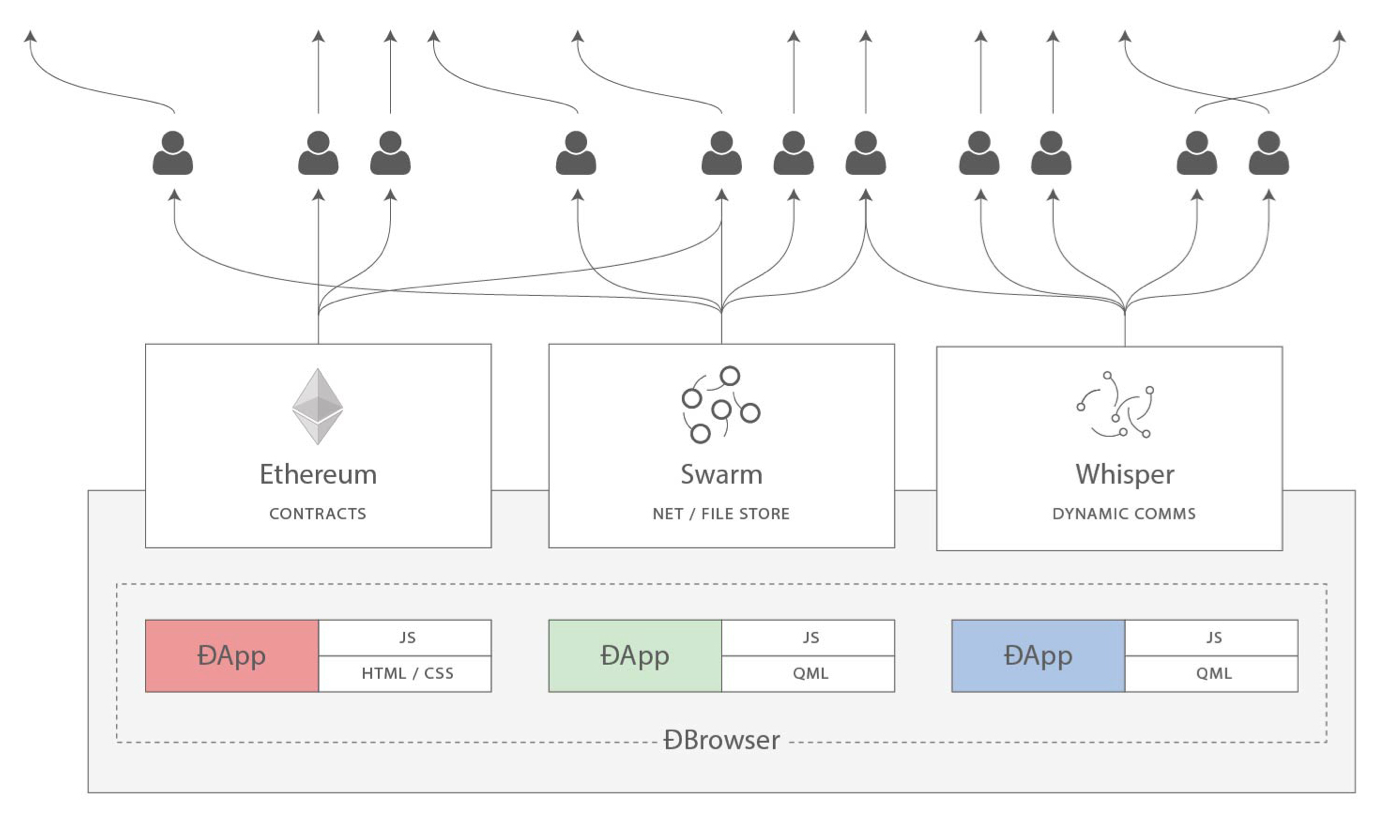
\includegraphics[width=1\columnwidth]{web3suite} 
\caption[Web3 web decentralizzato che utilizza smart contract e tecniche P2P]{Web3 web decentralizzato che utilizza smart contract e tecniche P2P}
\label{fig:web3siute} 
\end{figure}
%
Una \DH App è quindi un'applicazione per lo più, o interamente decentralizzata nei suoi vari aspetti: Software di back-end e frontend, archiviazione dati, comunicazioni messaggi e risoluzione dei nomi. Ognuno di questi può essere alquanto centralizzato o piuttosto decentralizzato. Ci sono diversi vantaggi che può portare una architettura decentralizzata di questo tipo:
\begin{itemize}
	\item \textbf{Elasticità:} la logica di business è controllata da uno smart contract, la back-end di una \DH App sarà completamente distribuita e gestita su blockchain, non sarà quindi vittima di possibili tempi di inattività.
	\item \textbf{Trasparenza:} la natura on-chain consente a tutti di visionare il codice delle varie funzioni.
	\item \textbf{Resistenza alla censura:} finchè un utente avrà accesso alla rete Ethereum sarà sempre in grado di interagire con una \DH App senza dipendere da nessun controllo centrale o qualsiasi fornitore di servizi.
\end{itemize}
Ma vediamo in dettaglio i vari aspetti di un'applicazione decentralizzata:

\subsubsection{Back-end (Smart Contract)}
Nelle \DH App, per archiviare la logica aziendale, si fa utilizzo degli smart contract sarà quindi così anche per lo stato di tale app. Possiamo pensare allo smart contract come quella componente che va a sostituire la back-end di un server in una normale applicazione. Da notare però che qualsiasi operazione eseguita con un contratto risulterà molto costosa per questo motivo si dovrà mantenere tale logica il puù minimale possibile e  soprattutto identificare quali aspetti della \DH App richiedono un'esecuzione affidabile e decentralizzata. Una considerazione importante di cui tener conto quando si procede con l'implementazione di uno smart contract è l'incapacità di modificare il codice una volta implementato. Può essere cancellato ma solamente se è stato programmato il codice operativo \lstinline|SELFDESTRUCT|. Ultima importante considerazione riguarda il design dell'architettura di uno smart contract. Un contratto monolitico molto grande può costare molto gas una volta eseguito. Si può scegliere di diminuire il carico integrando calcoli provenientri da fonti off-chain, ma questo significa che qualsiasi utilizzatore di questo servizio si drovrà fidare di tali fonti esterne.

\subsubsection{Frontend (Web User Interface)}
A differenza della logica di business di \DH App, che richiede di comprendere l'EVM e nuovi linguaggi come ad esempio Solidity, l'interfaccia lato client di una \DH App può utilizzare tecnologie web standard come HTML, CSS, JavaScript, ecc. Ciò consente quindi ad uno sviluppatore web tradizionale di utilizzare strumenti, librerie e framework famigliari. Le interazioni con Ethereum, come la firma di messaggi, l'invio di transazioni e la gestione di chiavi, sono spesso condotte attraverso il browser web, tramite un'estensione come MetaMask. Il frontend è in genere collegato a Ethereum tramite la libreria JavaScript \textit{web3.js}. 

\subsubsection{Data Storage}
A causa degli elevati costi del gas e del limite di gas a blocchi attualmente basso, i contratti intelligenti non sono adatti per archiviare o elaborare grandi quantità di dati. Pertanto, la maggior parte dei DApp utilizza servizi di archiviazione dati fuori catena, il che significa che memorizzano i dati ingombranti dalla catena Ethereum, su una piattaforma di archiviazione dati. La piattaforma di archiviazione dati può essere centralizzata (ad esempio, un tipico database cloud), oppure i dati possono essere decentralizzati, archiviati su una piattaforma P2P come l'IPFS o la piattaforma Swarm di Ethereum.
Lo storage P2P decentralizzato è ideale per archiviare e distribuire asset statici di grandi dimensioni come immagini, video e le risorse dell'interfaccia Web frontend dell'applicazione.

\subsubsection{Inter-Planetary File System (IPFS)}
E' un sistema decentralizzato per content-addressable per la distribuzione di oggetti memorizzati su di una rete P2P. "Content-addressable" significa che di ogni contenuto viene eseguito l'hash e questo hash verrà utilizzato per identificare tale file. Sarà così possibile recuperare qualsiasi file da qualsiasi nofo IPFS tramite il suo hash. IPFD mira a sostituire HTTP come protocollo per la consegna di applicazioni web.

\subsubsection{Swarm}
E' un altro sistema di archiviazione content-addressable simile a IPFS. Swarm è stato crato dalla Ethereum Fondation come parte della suite Go-Ethereum. Come IPFS, consente di archiviare file che vengono diffusi e reppliacti sui nodi Swarm. Il riferimento ai vari files viene eseguito sempre tramite hash e consente di accedere a un sito Web da un sistema P2P decentralizzato, anziché da un server Web centrale.

\subsubsection{Whisper}
Un altro componente importante di una qualsiasi applicazione è la comunicazione tra processi, il poter scambiare, quindi, messaggi tra applicazioni, diverse istanze dell'applicazione o tra i suoi vari utenti. Solitamente questo si ottiene facendo riferimento ad un server centrale, tuttavia esistono una varietà di alternative decentralizzate che offrono messaggistica su di una rete P2P. Il più importante protocollo di messaggistica P2P per \DH App risulta essere Whisper, che fa anche lui parte della suite Go-Ethereum.

\subsubsection{Ethereum Name Service (ENS)}
E' possibile progettare il miglior smart contract al mondo ma se non si fornisce una buona interfaccia per gli utenti, questi non saranno in grado di accedervi e quindi fruire del servizio. Su internet tradizionale, il Domani-Name-Sever (DNS) ci consente di navigare utilizzando dei nomi comprensibili all'uomo, mentre risolviamo quei nomi in indirizzi IP, recuperando così i contenuti cercati. Sulla blockchain Ethereum, l'Ethereum Naming System (ENS) risolve lo stesso problema, ma in modo decentralizzato. ENS è più di uno smart contract, è un \DH App fondamentale in sé, che offre un servizio di nomi decentralizzato. Inoltre, ENS è supportato da svariate \DH Apps per la registrazione e la gestione delle aste dei nomi registrati. ENS dimostra come le \DH App possono lavorare insieme. 

\section{La macchina virtuale di Ethereum}
Il cuore del protocollo Ethereum è appunto l'Ethereum Virtual Machine o EVM in breve. Come is può intuire da nome, si tratta di un motore di calcolo non molto diverso dalle macchine virtuali per il framework Microsoft .NET o di altri linguaggi compilati in bytecode come Java. Più in dettaglio, l'EVM è la parte di Ethereum che gestisce la distribuzione e l'esecuzione di contratti intelligenti. Le semplici transazioni di valore tra due EOA non devono coinvolgerlo ma si dovrà occupare di tutto ciò che comporta un aggiornamento di stato. L'EVM Ethereum può essere concepito come un computer decentralizzato globale contenente milioni di oggetti eseguibili, ciascuno con un proprio archivio di dati permanente. 
%
\begin{figure}
	\centering 
	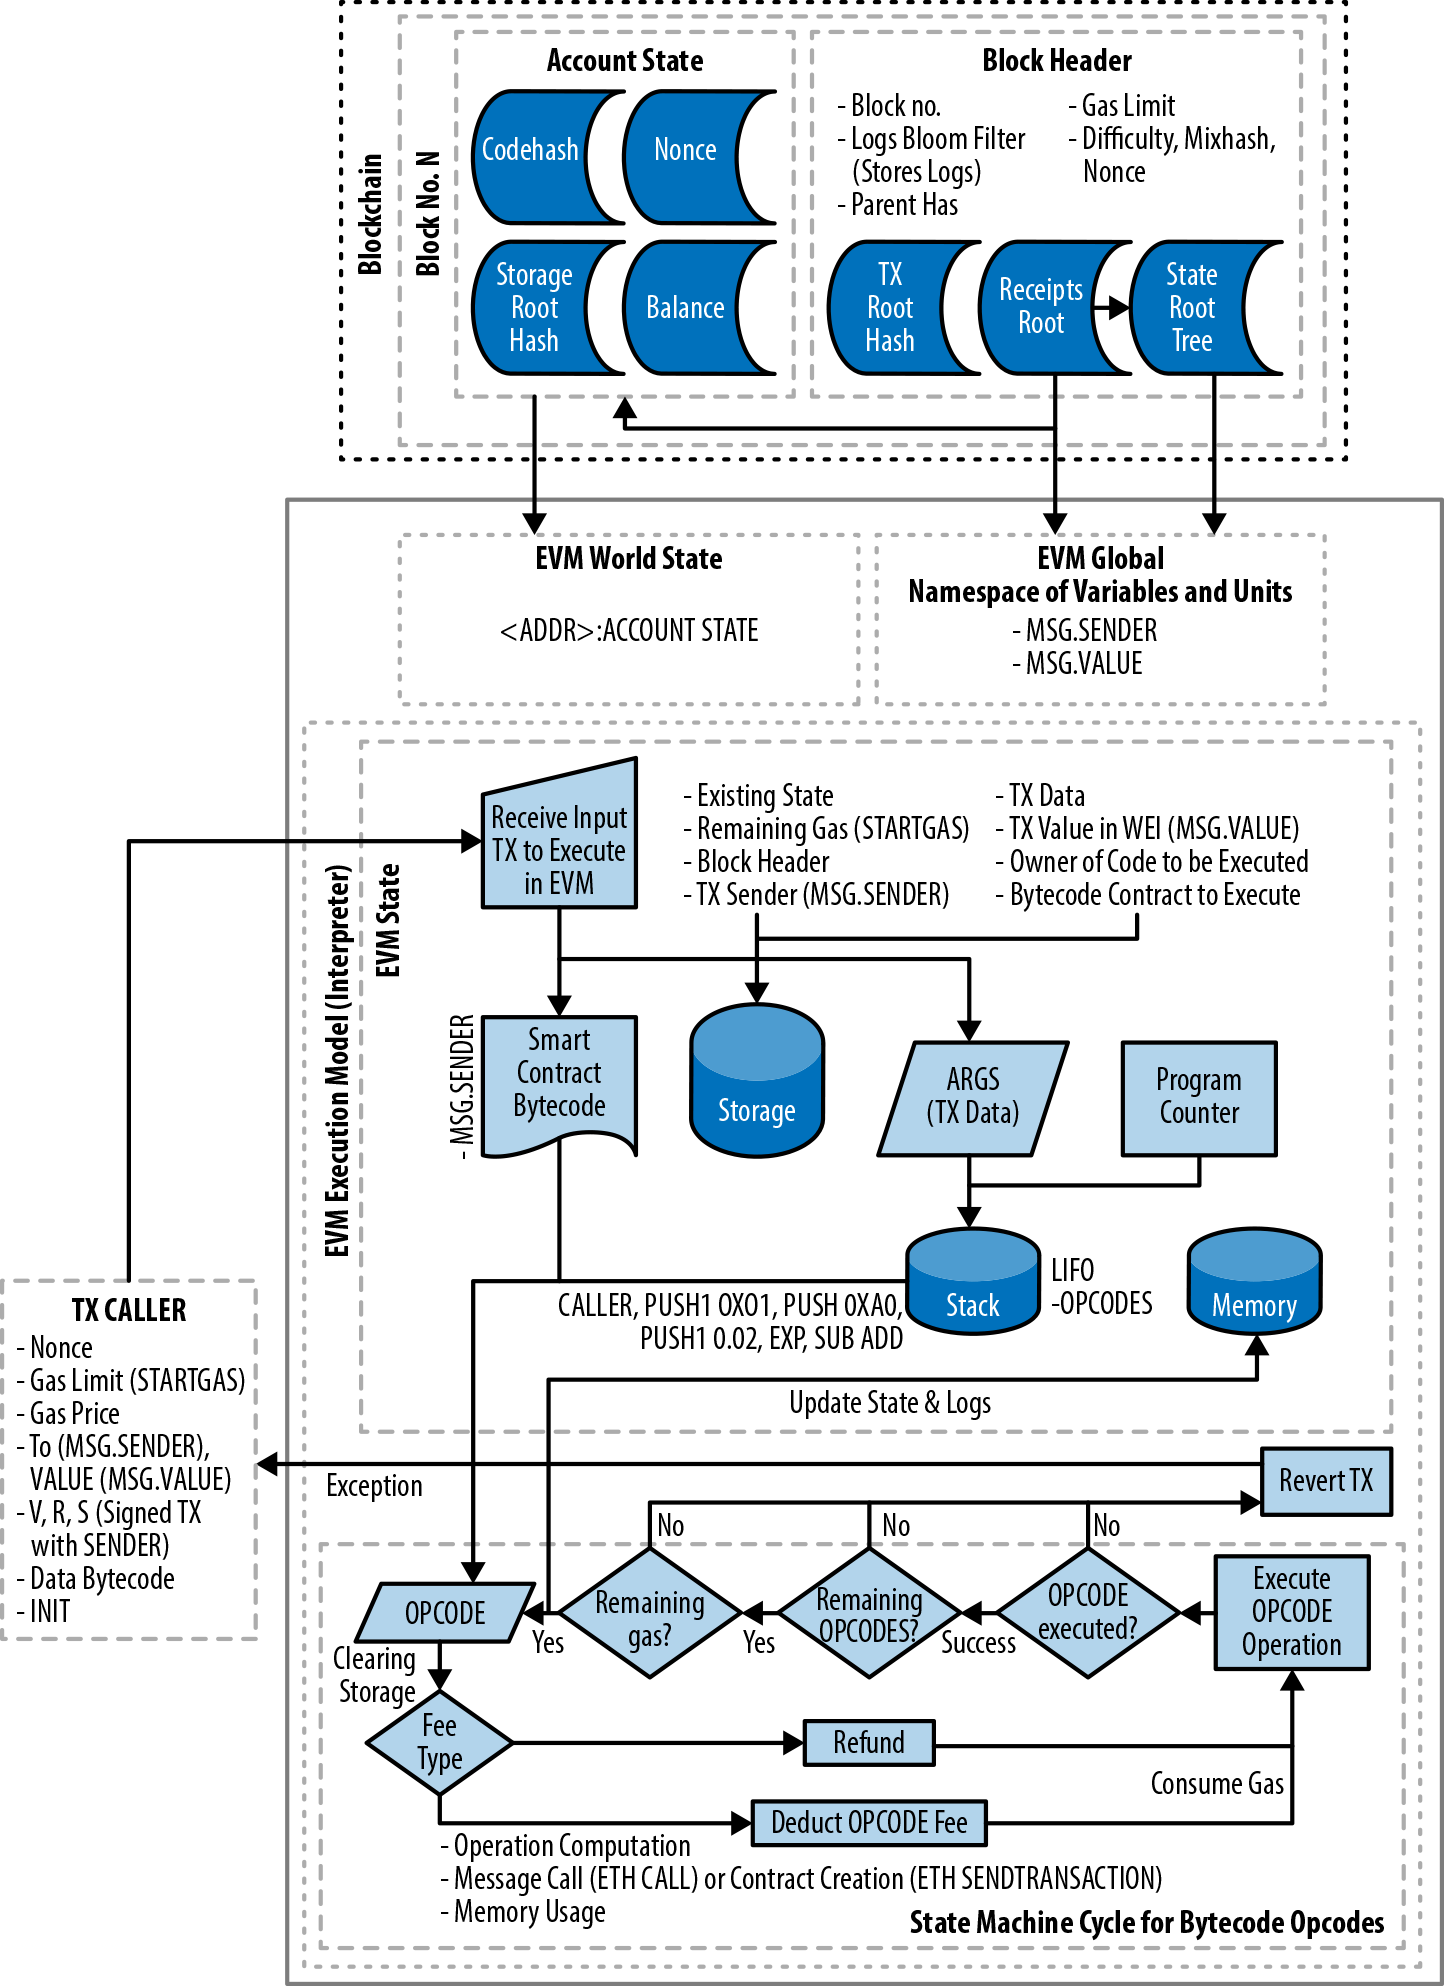
\includegraphics[width=1\columnwidth]{evm-architecture} 
	\caption[Architettura dell'EVM]{Architettura e contesto dell'EVM.}
	\label{fig:evm-architecture} 
\end{figure}
%
L'EVM è una macchina di Turing quasi completa, "quasi" perché tutti i processi in esecuzione sono limitati ad una numero finito di passaggi computazionali in base alla quantità di gas disponibile per ogni esecuzione, questo per garantire la terminazione di un qualsiasi codice sottoposto. L'architettura dell'EVM è basata su stack nel quale vengono salvati tutti i valori in memoria, ha diversi componenti di dati utilizzati:
\begin{itemize}
	\item La ROM di codice di programma immutabile, caricata con il bytecode del contratto intelligente da eseguire.
	\item Una memoria volatile, con ogni posizione esplicitamente inizializzata a zero.
	\item Una memoria permanente che fa parte dello stato di Ethereum, anch'essa inizializzata a zero.
\end{itemize}
Uno schema più completo lo si può vedere in Figura~\ref{fig:evm-architecture}.

\subsection*{Contronto con la tecnologia esistente}
Il termine "macchina virtuale" viene spesso applicato alla virtualizzazione di un computer reale, in genere da un "hypervisor" come VirtualBox o QEMU o da un'intera istanza del sistema operativo, come KVM di Linux. Questi devono fornire un'astrazione software dell'hardware effettivo, delle chiamate di sistema e altre funzionalità del kernel. EVM opera in un dominio molto più limitato: è solo un motore di calcolo e, in quanto tale, fornisce un'astrazione di solo computazione e archiviazione, simile, ad esempio, alle specifiche Java Virtual Machine (JVM). Da un punto di vista di alto livello, la JVM è progettata per fornire un ambiente di runtime che è indipendente dal sistema operativo o hardware host sottostante, consentendo la compatibilità su un'ampia varietà di sistemi. Linguaggi di programmazione di alto livello come Java o Scala (che usano JVM) o C\# (che usa .NET) sono compilati nel set di istruzioni bytecode della rispettiva macchina virtuale. Allo stesso modo, EVM esegue il proprio set di istruzioni bytecode, in cui vengono compilati i linguaggi di programmazione come LLL, Serpent, Mutan o Solidity.

\subsubsection{Stato di Ethereum}
Il compito dell'EVM è di aggiornare lo stato di Ethereum calcolando transizioni di stato valide come risultato dell'esecuzione del codice dello smart contract, come definito dal protocollo Ethereum. Quando una transazione richiama una funzione di un ceto smart contract, viene creata una EVM con tutte le informazioni richieste in relazione al blocco corrente a alla specifica transazione in elaborazione. In particolare l'EVM viene caricata con il codice del contratto chiamato, il program counter impostato a zero, lo storage locale viene caricato dallo storage dell'account di tale contratto, la memoria invece viene azzerata. Una variabile di particolare importanza è la fornitura di gas per l'esecuzione corrente, impostata sulla quantità di gas pagata dal mittente all'inizio della transazione. Mentre l'esecuzione del codice avanza, l'erogazione del gas viene ridotta in base al costo di ogni singola operazione eseguita. Se in qualsiasi momento venisse esaurito il gas, verrà lanciata l'eccezione Out-Of-Gas causando l'interruzione immediata dell'esecuzione e la transazione viene interrotta. Non vengono apportate modifiche allo stato precedente ad eccezione del nonce del mittente che viene incrementato, il gas speso per l'esecuzione fino all'interruzione non viene rimborsato e va a pagare il beneficiario del blocco per le risorse utilizzate fino al punto d'arresto. Tuttavia, se l'esecuzione viene completata correttamente, lo stato viene aggiornato per corrispondere alla versione dell'EVM in quel momento. 

\subsubsection{Turing completezza e Gas}
Come abbiamo già accennato, in termini semplici, un sistema o un linguaggio di programmazione è Turing completo se può eseguire qualsiasi programma. Un aspetto importante è che non possiamo dire, a priori, semplicemente guardando un programma, se tale programma terminerà o meno. Dobbiamo per forza procedere con l'esecuzione del programma ed attendere la sua terminazione per scoprirlo. Una delle possibilità è che il programma in questione non termini e questo ci porterebbe, in caso lo eseguissimo, ad attendere un tempo infinito. Questo si chiama halting problem, e sarebbe un grosso problema per Ethereum se non fosse affrontato. Se l'EVM eseguisse un programma di questo tipo diventerebbe inutilizzabile. Tuttavia, tramite l'utilizzo del Gas, c'è una soluzione: se dopo l'esecuzione di una quantità massima di calcolo , l'esecuzione non è terminata, tale procedura viene interrotta dall'EVM. Ciò rende l'EVM una macchina di Turing quasi completa dato che può eseguire qualsiasi programma inserito in essa, ma solo se termina entro una determinata quantità di calcolo. Questo limite non è fisso in Ethereum: puoi pagare per aumentarlo al massimo, chiamato il "limite del gas di blocco", e tutti possono concordare di aumentarlo nel tempo. 

\subsection*{Gas}
È l'unità di Ethereum per misurare le risorse computazionali e di archiviazione necessarie per eseguire azioni sulla blockchain di Ethereum. Diversamente da Bitcoin, le cui commissioni di transazione tengono conto solo delle dimensioni di una transazione in kilobyte, Ethereum deve tenere conto di ogni passo di calcolo eseguito dalle transazioni e dell'esecuzione del codice dello smart contract richiamato. ogni operazione eseguita da una transazione o contratto costa una quantità fissa di gas, vediamo alcuni esempi presi dal Yellow Paper di Ethereum:
\begin{itemize}
	\item La somma di due numeri costa 3 gas.
	\item Il calcolo di un hash Keccak-256 costa 30 gas + 6 gas per ogni 256 bit di dati sottoposti a hash.
	\item L'invio di una transazione costa 21.000 gas.
\end{itemize}
Prima di ogni operazione, l'EVM verifica che vi sia abbastanza gas da pagare per l'esecuzione dell'operazione. Se non c'è abbastanza gas, l'esecuzione viene interrotta e la transazione viene ripristinata. Se, invece, l'EVM raggiunge la fine dell'esecuzione con successo, senza esaurire il gas, il costo del gas utilizzato viene pagato al minatore come commissione di transazione, convertito in etere in base al prezzo del gas specificato nella transazione:
%
\begin{align*}
commissione Minatore &= costo Gas * prezzo Gas\\
gas Rimanente &= limite Gas - costo Gas\\
etere Rimborsato &= prezzo Rimanente Gas * Gas 
\end{align*}

\subsubsection{Costo del gas e prezzo del gas}
Mentre il conto del gas è misurato in base allo sforzo computazionale e di storage dell'EVM Ethereum, anche il gas stesso ha un prezzo in ether. Quando si esegue una transazione, il mittente specifica il prezzo del gas che è disposto a pagare (in etere) per ogni unità di gas, consentendo al mercato di decidere la relazione tra il prezzo dell'etere e il costo delle operazioni di calcolo (misurato in gas) :
%
\[ commissione Di Transazione = gas Totale Utilizzato * prezzo Gas Pagato \]
%
Quando si costruisce un nuovo blocco, i minatori della rete Ethereum possono scegliere tra le transazioni in sospeso selezionando quelle che offrono di pagare un prezzo del gas più alto. Offrire un prezzo del gas più elevato incentiverà pertanto i minatori a includere la transazione e a confermarla più rapidamente. In pratica, il mittente di una transazione imposterà un limite di gas superiore o uguale alla quantità di gas che si prevede di utilizzare. Se il limite di gas è impostato su un valore superiore alla quantità di gas consumato, il mittente riceverà un rimborso dell'importo in eccesso, in quanto i minatori sono solo compensati per il lavoro effettivamente svolto. Deve essere chiara la distinzione tra il costo del gas e il prezzo del gas:
\begin{itemize}
	\item Il costo del gas è il numero di unità di gas necessarie per eseguire una determinata operazione.
	\item Il prezzo del gas è la quantità di ether che si è disposti a pagare per unità di gas quando si invia la transazione alla rete Ethereum.
\end{itemize}

\subsubsection{Costi negativi del gas}
Ethereum incoraggia la cancellazione delle variabili e degli account di archiviazione usati rimborsando parte del gas utilizzato durante l'esecuzione del contratto. Nell'EVM esistono due operazioni con costi negativi di gas:
\begin{itemize}
	\item La cancellazione di un contratto \lstinline|SELFDESTRUCT| vale un rimborso di 24.000 gas.
	\item La modifica di un indirizzo di archiviazione da un valore diverso da zero a zero (\lstinline|SSTORE [x] = 0|) vale un rimborso di 15.000 gas.
\end{itemize}
Per evitare lo sfruttamento di tale meccanismo di rimborso, il rimborso massimo per una transazione è pari alla metà della quantità totale di gas utilizzato.

\subsubsection{Block gas limit}
Il limite del gas di blocco è la quantità massima di gas che può essere consumata da tutte le transazioni in un blocco e limita quindi il numero di transazioni che possono essere contenute in un blocco. Un semplice esempio, con cinque transazioni, è riportato in Tabella~\ref{tab:transactions-cost}. Se supponiamo che il limite massimo di gas per blocco è impostato a 180.000, notiamo che non tutte le transazioni possono essere inserite in un unico blocco, o meglio, solo quattro di quelle riportate in tabella saranno incluse nello stesso blocco. Se un minatore tenta di includere una transazione che richiede più gas rispetto al limite di gas di blocco corrente, il blocco verrà rifiutato dalla rete. Come per le transazioni Bitcoin, è possibile che diversi minatori selezionino combinazioni diverse, principalmente perché ricevono transazioni dalla rete in un ordine diverso. Il limite di gas di blocco sulla rete principale Ethereum è 8 milioni di gas al momento della stesura secondo https://etherscan.io, il che significa che circa 380 transazioni di base ($\sim$ 21.000 gas cdu) potrebbero rientrare in un singolo blocco.
\begin{table}[]
	\centering
	\begin{tabular}{|c|c|c|c|c|c|}
		\hline
		\textbf{Tran.1} & \textbf{Tran.2} & \textbf{Tran.3} & \textbf{Tran.4} & \textbf{Tran.5} & \textbf{Tot.}\\ \hline
		30.000 & 30.000 & 40.000 & 50.000 & 50.000 & 200.000\\ \hline \hline
		\ding{51} & \ding{51} & \ding{51} & \ding{51} & \ding{55} & 150.000 \\ \hline
		\ding{51} & \ding{51} & \ding{55} & \ding{51} & \ding{51} & 160.000 \\ \hline
		\ding{51} & \ding{55} & \ding{51} & \ding{51} & \ding{51} & 170.000 \\ \hline
	\end{tabular}
	\caption{Esempi di transazioni con relativi costi}
	\label{tab:transactions-cost}
\end{table}

\section{Il consenso}
Le regole di consenso sono tutte quelle regole che tutti devono accettare affinché il sistema operi in modo decentrato, ma deterministico. In informatica, il termine "consenso" è correlato ad un più ampio problema di sincronizzazione dello stato nei sistemi distribuiti, in modo tale che i diversi partecipanti in un sistema distribuito siano tutti d'accordo su un singolo stato a livello di sistema. Questo è chiamato \textit{raggiungimento del consenso}. Quando queste funzioni decentralizzate di consenso permettono di salvare e mantenere memoria di uno stato, può diventare problematico affidarsi solamente alla fiducia per garantire che le informazioni derivanti dagli aggiornamenti di stato siano corrette. Questa sfida è particolarmente pronunciata nelle reti decentralizzate perché non esiste un'entità centrale che decida per noi. Senza un arbitro affidabile, eventuali disaccordi o differenze devono essere riconciliati con altri mezzi e gli algoritmi di consenso sono appunto il meccanismo utilizzato per riconciliare sicurezza e decentralizzazione. Nelle blockchain, il consenso è una proprietà critica del sistema dal momento in cui ci sono soldi in palio. Tale consenso quindi è destinato a produrre un sistema di regole severe ma senza governanti. La capacità di arrivare al consenso attraverso una rete distribuita, in condizioni contraddittorie, senza controllo centralizzato è il principio fondamentale di tutti i blockchain pubblici aperti. Per affrontare questa sfida e mantenere la proprietà di valore del decentramento, la comunità continua a sperimentare diversi modelli di consenso.

\subsection{Consenso tramite Proof-of-Work}
Il creatore della blockchain Bitcoin, ha inventato un algoritmo di consenso chiamato proof of work (PoW). Il termine colloquiale per PoW è "mining" e questo crea non pochi equivoci circa lo scopo del minatore. Spesso, infatti, si presuppone che lo scopo del mining sia quello di creare della nuova valuta, dal momento in cui tale parola rispecchia nella realtà un lavoro che comporta l'estrazione di un minerale prezioso, in questo caso equiparato alla valuta che si ricava. Il vero scopo del mining, così come per tutti gli altri modelli di consenso, è quello di proteggere la blockchain mantenendo il controllo sul sistema decentralizzato diffondendolo al maggior numero di partecipanti possibili. Il conio di nuova moneta a lavoro terminato è solamente un incentivo per coloro che contribuiscono alla sicurezza del sistema, un mezzo per un fine.

Nel consenso di PoW è presente anche una corrispondente \textit{punizione} che risulta il costo dell'energia richiesta per prendere parte a tale mining. Se i partecipanti non seguono le regole e assegnandosi la ricompensa, rischiano i fondi per il pagamento dell'elettricità spesa fino a quel momento. Pertanto, il consenso di PoW è un attento equilibrio tra rischio e rendimento che spinge i partecipanti a comportarsi onestamente per interessi personali. Ethereum è attualmente una blockchain di tipo PoW con lo stesso obiettivo di base, cioè assicurare la blockchain mentre si decentralizza il controllo. Ethereum implementa un versione leggermente diversa da quella di Bitcoin e si chiama Ethash.

\subsection{Consenso tramite Proof-of-Stake}
Storicamente, la Proof-of-Work non fu il primo algoritmo di consenso proposto fu anticipato infatti dal Proof-of-Stake. Dopo il successo di Bitcoin, molte blockchain hanno emulato la PoW, non approcciandosi quindi alla PoS. Fin dall'inizio, i fondatori di Ethereum speravano di riuscire a migrare verso la Proof-of-Stake dal momento in cui PoW ha un problema ben noto: la \textit{Bomba di Difficoltà}. Quest'ultima infatti rappresenta il fatto che si tende a rendere sempre più difficile il calcolo della PoW, a causa della maggiore potenza computazionale della rete, che col passare del tempo forzerà Ethereum al passaggio verso un sistema PoS. Al momento della stesura di questa Tesi, Ethereum utilizza ancora la proof-of-work, ma la ricerca verso un'alternativa proof-of-stake è in via di completamento. L'algoritmo PoS per Ethereum prenderà il nome di \textit{Casper}. L'introduzione di quest'ultimo in sostituzione dell'attuale \textit{Ethash} è stata posticipata più volte negli ultimi due anni. In generale un algoritmo PoS funziona come segue. La blockchain tiene traccia di una serie di validatori, e chiunque detenga della criptovaluta, nel caso di Ethereum l'ether, può diventare validatore inviando una speciale transazione che andrà a bloccare l'ether in un deposito. Tali validatori, a turno, propongono e votano il successivo blocco valido, e il peso del voto di ciascun validatore dipende dalla dimensione del suo deposito. E' importante sottolineare che un validatore rischia di perdere il deposito se il blocco su cui impila verrà rifiutato dalla maggior parte dei validatori. Viceversa, i validatori guadagnano una piccola ricompensa, sempre proporzionale alla loro quota depositata, per ogni blocco accettato dalla maggioranza. Quindi anche PoS forza i validatori ad agire onestamente e seguire le regole del consenso.

\subsection*{Ethash: L'algoritmo PoW di Ethereum}
Ethash è l'algoritomo proof-of-work di Ethereum ed utilizza un'evoluzione dell'algoritmo \textit{Dagger-Hashimoto}, che è una combinazione dell'algoritmo \textit{Dagger} di Vitalik Buterin e dell'algoritmo \textit{Hashimoto} di Thaddeus Dryja. Ethash dipende dalla generazione e dall'analisi di un grande set di dati, noto come un grafo aciclico diretto, o DAG, che aveva una dimensione iniziale di circa 1 GB e continuerà a crescere lentamente e linearmente in dimensioni, aggiornandosi una volta ogni epoca (30.000 blocchi o circa 125 ore). Lo scopo del DAG è di rendere l'algoritmo di Ethash PoW dipendente dal mantenimento di una struttura di dati ampia e frequentemente utilizzata. Questo a sua volta ha lo scopo di rendere Ethash resistente all'ASIC, il che significa che sarà più difficile realizzare apparecchiature per l'estrazione su circuiti integrati specifici per applicazioni (ASIC) che siano ordini di grandezza più veloci di una GPU. In questo modo i fondatori di Ethereum evitano che avvenga un accentramento di estrazione del PoW da parte di coloro che hanno accesso a fabbriche specializzate di questo tipo, il che porterebbe al dominio della potenza di estrazione minando la sicurezza dell'algoritmo di consenso. L'utilizzo di GPU consumer-level per l'esecuzione del PoW sulla rete Ethereum significa che più persone in tutto il mondo possono partecipare al processo di mining. Più sono i minatori indipendenti, più decentralizzato sarà il potere minerario, il che significa che possiamo evitare una situazione come in Bitcoin, dove gran parte della potenza mineraria è concentrata nelle mani di alcune grandi organizzazioni di mining Bitcoin.
% !TEX encoding = UTF-8
% !TEX TS-program = pdflatex
% !TEX root = ../Tesi.tex
% !TEX spellcheck = it-IT

%************************************************
\chapter{Takamaka}
\label{takamaka-chapter}
%************************************************
Questo capitolo è tratto dall'articolo \cite{paper-takamaka:spoto}, scritto dal docente Nicola Fausto Spoto, nel quale si definisce un framework per la programmazione in Java, di smart contract su blockchain. Tale framework sarà costituito da una routine limitata e da un set di classi che dovranno essere mantenute su blockchain per essere utilizzati dai metodi di contratto e per la misurazione del gas. Questo framework permette inoltre di sfruttare le competenze e gli strumenti già esistenti del mondo Java, al fine di  costruire smart contract in modo semplice e confortevole. 

\section{Un Framework Java per Smart Contract}
Takamaka\footnote{Takamaka è una valle nell'isola della Réunion Francese, dove una rete di cascate converge in un fiume. Questo è simile ai contratti intelligenti Takamaka, cioè a oggetti distinti che collaborano su uno spazio di archiviazione globale condiviso nella blockchain.} è un framework Java per la programmazione di smart contract. Più in particolare, questo framework, è un sottoinsieme di Java, supportato dalla sua libreria runtime \lstinline|takamaka.jar| che include le poche classi che descriveremo in seguito. È anche supportato da una selezione di metodi white-listed della libreria standard di Java. Questi sono metodi la cui esecuzione risulta deterministica. Per esempio, i metodi per la concorrenza non sono permessi, non saranno quindi white-listed in quanto potrebbero portare a comportamenti non deterministici. Il software Takamaka è scritto, verificato ed eseguito come segue:
\begin{description}
	\item[Sviluppo] 
		Le applicazioni Takamaka sono sviluppate come normali applicazioni Java, incluso \lstinline|takamaka.jar|. Non esiste un ambiente di sviluppo speciale per Takamaka. Infatti, è possibile utilizzare qualsiasi IDE o anche solo un compilatore a riga di comando. Il risultato, in ogni caso, sarà l'archivio \lstinline|app.jar| dell'applicazione in fase di sviluppo.
	\item[Verifica] 
		Le classi all'interno di \lstinline|app.jar| vengono verificate per fare in modo che facciano riferimento solo a metodi white-listed. Inoltre, questo passaggio viene verificato che le classi in memoria abbiano componenti di tipo consentito (Sezione 6).
	\item[Installazione]
		L'archivio \lstinline|app.jar| viene installato sulla blockchain, attivando una transazione che installa un jar (Sezione 3).
	\item[Strumentazione]
		Le classi all'interno di \lstinline|app.jar| vengono strumentate. In particolare, le classi di memoria subiscono una trasformazione a livello bytecode che consente ai loro oggetti di essere caricati lentamente in RAM durante l'esecuzione di una transazione e mantenerli aggiornati sulla blockchain, alla sua fine, se sono stati aggiornati (Sezione 6). Inoltre, nel codice viene iniettato un aspetto di misurazione del gas (Sezione 9).
	\item[Esecuzione] 
		Le classi definite in \lstinline|app.jar|, incluse le classi di contratto, vengono istanziate attraverso una transazione che esegue il loro costruttore (Sezione 5). Il risultante \textit{storage reference} può essere usato per richiamare i metodi del nuovo oggetto.
\end{description}
Quello che segue è un esempio di un contratto di crowdfunding scritto a Takamaka. Questo contratto permette a dei finanziatori di versare fondi da devolvere per una campagna. Una volta raggiunta la soglia di una certa campagna i fondi possono essere sbloccati. Tale implementazione consiste in due classi. Vediamo la prima, \lstinline|Founder.java|.
%
\begin{lstlisting}
	import takamaka.lang.Contract;
	import takamaka.lang.Storage;
	
	public class Funder extends Storage {
		private final Contract who;
		private final int amount;
		
		public Funder(Contract who, int amount) {
			this.who = who;
			this.amount = amount;
		}
	}
\end{lstlisting}
%
Definisce il finanziatore di una campagna, cioè un contratto che riporta la quantità di denaro che un determinato \lstinline|Founder| intende devolvere per una certa campagna. Dato che questi oggetti devono essere persistenti in blockchain, la classe \lstinline|Founder| deve estendere \lstinline|takamaka.lang.Storage|. Vediamo ora la seconda classe, \lstinline|CrowdFunding.java|:
%
\begin{lstlisting}
	import takamaka.lang.Contract;
	import takamaka.lang.Payable;
	import takamaka.lang.Storage;
	import takamaka.util.StorageList;
	
	public class CrowdFunding extends Contract {
		private final StorageList<Campaign> campaigns = new StorageList<>();  ■\label{line:storage_list}■
		
		public void newCampaign(Contract beneficiary, int goal) {
			campaigns.add(new Campaign(beneficiary, goal));
		}
		
		public @Payable @Entry void contribute(int amount, int campaignID) {  ■\label{line:payable}■
			campaigns.elementAt(campaignID).addFunder(payer(), amount);
		}
		
		public boolean checkGoalReached(int campaignID) {
			return campaigns.elementAt(campaignID).payIfGoalReached();
		}
		
		private class Campaign extends Storage {  ■\label{line:campaign_is_storage}■
			private final Contract beneficiary;
			private final int fundingGoal;
			private final StorageList<Funder> funders = new StorageList<>();
			private int amount;
		
			private Campaign(Contract beneficiary, int fundingGoal) {
				this.beneficiary = beneficiary;
				this.fundingGoal = fundingGoal;
			}
		
			private void addFunder(Contract who, int amount) {
				funders.add(new Funder(who, amount)); this.amount += amount;
			}
		
			private boolean payIfGoalReached() {
				if (amount >= fundingGoal) {
					pay(beneficiary, amount); ■\label{line:pay}■
					amount = 0;
					return true;
				}
				else
					return false;
			}
		}
	}
\end{lstlisting}
%
Rappresenta il contratto del coordinatore del crowdfunding, garantisce che i fondi dedicati ad una campagna non possano essere negati una volta raggiunto l'obiettivo. Consente di avviare una nuova campagna tramite \lstinline|new Campaign|, che mantiene il proprio astato all'interno dell'elenco di campagne avviate. Tale elenco utilizza la classe \lstinline|takamaka.util.StorageList|, che estende \lstinline|Storage|, e può quindi essere presente in blockchain. È possibile contribuire ad una certa campagna tramite \lstinline|contribute|. Viene data la possibilità di verificare se l'obiettivo della campagna è stato raggiunto tramite \lstinline|checkGoalReached|. La campagna è implementata tramite la classe interna \lstinline|Campaign|, in questo modo può fare riferimento al contratto esterno e consentendo di richiamare il metodo \lstinline|pay| del contratto (riga \ref{line:pay}), che trasferisce una data somma di denaro ad un determinato beneficiario. Questo metodo della classe \lstinline|Contract| è \lstinline|final| e di conseguenza non può essere ridefinito, evitando così qualsiasi rischio di reentrancy. È interessante notare che \lstinline|Campaign| estende \lstinline|Storage| (riga \ref{line:campaign_is_storage}) perchè le sue istanze sono contenute all'interno dell'elenco \lstinline|campaigns|, (riga \ref{line:storage_list}) e di conseguenza deve essere persistente nella blockchain.
Alla riga \ref{line:payable} sono presenti le annotazioni \lstinline|@Payable @Entry|. \lstinline|@Entry| indica che si tratta di un punto d'accesso inter-contrattuale e limita il metodo ad appartenere ad una classe che estende \lstinline|takamaka.lang.Contract|. All'interno dei metodi \lstinline|@Entry| è possibile chiamare il metodi \lstinline|payer|, che restituisce il contratto chiamato. In generale, il programmatore utilizzerà \lstinline|@Entry| quando desidera identificare il contratto del metodo richiamato o desidera ricevere denaro da tale contratto. L'annotazione \lstinline|@Payable| può essere aggiunta solamente ad un costruttore o metodo \lstinline|@Entry|. Ciò significa che quest'ultimo riceverà denaro dal contratto \lstinline|payer|. Takamaka trasferirà automaticamente la somma specificata da \lstinline|payer| al contratto di destinazione.

\section{Salvare i file Jar sulla Blockchain}
Takamaka permette di conservare i jars sulla blockchain. Ci sono transazioni che memorizzano jar con riferimenti alle sue dipendenze, se presenti. Il meccanismo ricorda quello che viene fatto attualmente in Ivy o Ant: per memorizzare un jar $j$, viene creata una transazione $t$, che aggiunge $j$ alla blockchain, assieme ai riferimenti ad altre transazioni in cui le sue dipendenze, $d_1, \dots, d_n$, se presenti, sono state precedentemente memorizzate sulla blockchain. Il riferimento a $t$ può quindi essere utilizzato per memorizzare altri jars che dipendono da $j$. Le dipendenze ricorsive tra jars non sono consentite. Le eventuali dipendenze possono essere risolte in modo transitivo o non transitivo. Questo è legato alla costruzione del classpath per l'installazione dello smart contract (Sezione 5). Per memorizzare $j$ sulla blockchain, la transazione memorizzerà i seguenti dati:
%
\[\langle j, *d_1, t_1, \dots, *d_n, t_n \rangle\]
%
dove $*d_1$ è il riferimento al jar $i$-esimo da cui dipende $j$, $t_1$ è invece un booleano che afferma se la dipendenza è transitiva o meno. 

\section{Storage}
Uno smart contract ha un proprio \textit{stato}, costituito dai valori dei suoi campi e dagli oggetti raggiungibili da essi, in modo ricorsivo. Tale stato è persistente sulla blockchain, dopo la creazione di un contratto o dopo l'esecuzione di una transazione contrattuale. Per efficienza vengono mantenuti solo gli aggiornamenti dello stato, anziché lo stato completo. Si noti che contratti distinti potrebbero condividere parte del loro stato, quindi una transazione su di un contratto potrebbe andare a modificare oggetti visibili ad un altro contratto, questo è uno standard per Java. Può essere usato come forma di comunicazione tra con tratti sulla blockchain. Gli stati di tutti i contratti installati su blockchain formano una struttura ad heap, persistente, chiamata \textit{storage}. I riferimenti agli oggetti di archiviazione sono chiamati \textit{storage references} e hanno la forma:
%
\[\langle block\_number, \mathit{transaction \_number}, \mathit{progressive} \rangle \]
%
questo significa che farà riferimento all'oggetto $progressive$-esimo istanziato durante l'esecuzione della transazione $transaction\_number$-esima, all'interno del blocco $block\_number$-esimo.

Quando viene eseguita una transazione di contratto, lo stato del contratto viene caricaro in RAM, con i campi che contengono i riferimenti di memoria che riflettono i riferimenti di archiviazione dello stato persistente. Quindi una transazione viene eseguita all'interno di una standard \textit{Java Virtual Machine}, in RAM. Alla fine dell'esecuzione, tutti gli aggiornamenti dell'heap allo stato del contratto vengono resi persistenti nello storage. Questo avviene in modo automatico ed in maniera trasparente per il programmatore. Ciò significa che gli oggetti Java, in RAM, che possono essere persistenti sullo storage, come tutte le classi che implementano un contratto, devono avere la capacità di identificare gli eventuali aggiornamenti ai loro campi, in modo efficiente. Per questo motivo, Takamaka richiede che gli oggetti storage estendano \lstinline|takamaka.lang.Storage|: solo gli oggetti che estendono tale classe possono essere persistenti nello storage. Tutti questi aggiornamenti saranno memorizzati nello storage come \textit{storage updates}. Quest'ultimi saranno rappresentati da triple del tipo $\langle ref, sig, new\_value \rangle$, il che significa che il campo con firma $sig$ dell'oggetto il cui riferimento in memoria $ref$ è stato aggiornato al $new\_value$ indicato. Gli aggiornamenti possono essere compattati così da ridurne le dimensioni di archiviazione.

Supponiamo che i client espongano la blockchain come oggetto accessibile tramite \lstinline|Blockchain.getInstance()|, con i seguenti metodi:

\vspace{1ex}
\noindent
\lstinline|getCurrentTransaction()|:
	restituisce la transazione corrente in esecuzione.
	
\vspace{1ex}
\noindent
\lstinline|getTopmostBlock()|:
	produce il blocco più in alto del blockchaind.

\vspace{1ex}
\noindent
\lstinline|deserialize(r)|:
	produce un oggetto $o$ che è la deserializzazione dalla blockchain del riferimento di memoria $r$.
	
\vspace{1ex}
\noindent
\lstinline|deserializeLastUpdateFor(r, "C.f:D")|:
	restituisce l'oggetto $o'$ tenuto all'interno del campo di riferimento \lstinline|Cf: D| (\textit{i.e.} il campo \lstinline|f|, definito nella classe \lstinline|C| e avente tipo di riferimento \lstinline|D|) di un oggetto container il cui riferimento nello storage è $r$.
	
\section{Creazione di uno smart contract}
L'istanziazione una classe $C$, possibilmente implementando uno smart contract e quindi estendendo \lstinline|takamaka.lang.Contract| viene attivata da un utente della blockchain e consiste nella creazione di un'istanza di $C$. Il costruttore di $C$ viene chiamato con alcuni parametri. Lo stato risultante del contratto risulterà persistente in blockchain, come una set di aggiornamenti di storage. Questo set contiene gli aggiornamenti che portano all'ultima istanza di $C$, ma c'è la possibilità che contenga aggiornamenti di altri oggetti di storage utilizzati nell'implementazione di $C$. 

Per istanziare $C$, è necessario specificare $*j$, il riferimento al jar fornendo così il classpath per l'esecuzione del costruttore $C$ ed un valore booleano $t$ che specifica se le dipendenze del jar devono essere incluse in modo transitivo. Inoltre deve essere specificata una firma $sig = C(\dots)$ del costruttore, ed infine i parametri $pars$ che tale costruttore deve specificare, se ce ne sono. Quindi un client riceve la richiesta di creare un nuovo contratto come: $\langle *j, t, sig, pars \rangle$. I parametri $pars$ possono essere valori primitivi, dati dalla serializzazione Java, oppure riferimenti ad oggetti nello storage. L'esecuzione del costruttore comporterà degli aggiornamenti allo stato, compresi quelli per inizializzare il nuovo oggetto. Tuttavia potrebbero essere modificati anche altri stored object, se raggiungibili dai parametri passati al costruttore. In conclusione, la transazione aggiunta alla blockchain consiste nella tupla $\langle *j, t, sig, pars, result, updates \rangle$, dove $result$ è la referenza allo storage al nuovo oggetto $o$ della classe $C$ e $update$ colleziona tutti gli aggiornamenti allo storage, compresi quelli che inizializzano i campi dell'oggetto $o$. Nel caso particolare in cui l'esecuzione del costruttore termina con un'eccezione, $result$ conterrà la descrizione di tale eccezione e $update$ non contiene modifice ad $o$, se è irraggiungibile.

\section{Classi storage e la loro strumentazione}
Le classi storage estendono \lstinline|takamaka.lang.Storage|. Poiché solo tali classi possono essere mantenute in modo permanente in blockchain, ne consegue che i loro campi devono essere primitivi o, in modo ricorsivo, avere una storage class. La classe \lstinline|takamaka.lang.Storage| implementa dei meccanismi base per tenere traccia del riferimento nello storage dell'istanza. Ciò significa che un oggetto nello storage $o$, quando sarà in RAM, potrebbe essere presente l'oggetto deserializzato $o'$, già presente in blockchain, in quel caso il suo campo \lstinline|onStorage| è settato a true, e i suoi campi \lstinline|blockNumber|, \lstinline|transactioNumber| e \lstinline|progressive| sono i riferimenti nello storage di $o'$. Ma $o$ potrebbe non essere ancora presente in blockchain e quindi rappresentare un nuovo storage object, istanziato durante l'esecuzione di una transazione, che potrebbe essere successivamente conservato su blockchain, al termine della transazione. In questo caso il campo \lstinline|inStorage| varrà false e i campi \lstinline|blockNumber|, \lstinline|transactionNumber| e \lstinline|progressive| conterranno i riferimenti nello storage assegnati ad $o'$ nel caso di mantenimento in blockchain. Per rappresentare queste due alternative, \lstinline|takamaka.lang.Storage| ha due costruttori.
%
\begin{lstlisting}
	// constructor used by the programmer to build objects not yet in storage
	protected C() {
		this.inStorage = false;
		this.storageReference = new StorageReference(
			blockchain.getTopmostBlock().getNumber(),
			blockchain.getCurrentTransaction().getNumber(),
			nextProgressive++ );
	}
	...
	// constructor used by Takamaka to build objects deserialized from storage
	protected C( StorageReference storageReference ) {
		this.inStorage = true;
		this.storageReference = storageReference;
	}
	// vedi l'intera classe Storage sul paper Takamaka ■\cite{paper-takamaka:spoto}■
\end{lstlisting}
%
Takamaka al termine della transazione, chiama $o$.\lstinline|extractUpdates(updates)|, su tutti gli oggetti $o$ raggiungibili dallo stato del contratto o dai parametri di transazione. Raccoglie quindi in \lstinline|update| gli aggiornamenti di $o$ di cui si dovrà tener traccia nello storage e restituisce la storage reference di $o$ nella blockchain. La classe \lstinline|takamaka.lang.Storage|, non definisce i campi che appartengono allo stato di un oggetto nello storage: saranno le sottoclassi a ridefinire \lstinline|extractUpdate| per creare gli update. I programmatori scriveranno le classi di storage come normali classi Java estendendo \lstinline|takamaka.lang.Storage|. Il codice di tali classi subirà poi una trasformazione automatica prima di essere eseguito, per consentire:
\begin{enumerate}
	\item la generazione degli update alla fine di ogni transazione: gli oggetti nello storage hanno campi strumentati che consentono a Takamaka di identificare le parti del loro stato che ha subito modifiche.
	\item la deserializzazione, su richiesta, di storage object a cui si accede durante una transazione. Infatti, è teoricamente possibile caricare in RAM l'intero stato di un contratto, in modo ricorsivo, prima di una transazione. Ma tutto ciò sarebbe poco pratico dato che tale stato potrebbe essere molto grande e, inoltre, la deserializzare oggetti storage in RAM è un'operazione lenta poiché richiede l'accesso alla blockchain.
\end{enumerate}
Per esemplificare la trasformazione, supponiamo che un programmatore scriva la seguente classe:
%
\begin{lstlisting}[numbers=none,frame=none]
	public class C extends Storage {
		private D f1;
		private int f2;
		public C(pars) {
			// implicit call to super() here
			body
		}
		methods
	}
\end{lstlisting}
%
Tale classe viene compilata in java bytecode. Prima della sua esecuzione, viene automaticamente trasformato nel bytecode corrispondente al seguente sorgente:
%
\begin{lstlisting}
	public class C extends Storage {
		private D f1;
		private D oldF1;
		private boolean f1AlreadyLoaded;
		private int f2;
		private int oldF2;
	
		public C(pars) {
			// implicit call to super() here
			instrumented body     ■\label{line:instrumented1}■
		}
	
		// constructor added for deserialization from storage
		public C(StorageReference storageReference, int _f2) { ■\label{line:constructor_deserialization_C}■
			super(storageReference);
			f2 = oldF2 = _f2;
		}
		
		// method that replaces f1 read operations
		private D getF1() {
			ensureLoadedF1();     ■\label{line:ensure1}■
			return f1;
		}
		
		// method that replaces f1 write operations
		private void putF1(D _f1) {
			ensureLoadedF1();     ■\label{line:ensure2}■
			f1 = _f1;
		}
		
		private void ensureLoadedF1() {
			if (inStorage && !f1AlreadyLoaded) {
				oldF1 = (D) blockchain.deserializeLastUpdateFor(
					storageReference, "C.f1:D");
				f1AlreadyLoaded = true;
			}
		}
		
		public StorageReference extractUpdates(Updates updates) {
			StorageReference _this = super.extractUpdates(updates);
			if (!inStorage || f1 != oldF1)
				updates.add(<_this, "C.f1:D", recursiveExtract(f1, updates)>); ■\label{line:recursion1}■
			recursiveExtract(oldF1, updates); ■\label{line:recursion2}■
			if (!inStorage || f2 != oldF2)
				updates.add(<_this, "C.f2:int", f2>);
		
			return _this;
		}
		
		instrumented methods      ■\label{line:instrumented2}■
	}
\end{lstlisting}
%
Quando uno storage object viene deserializzato dallo storage, i suoi campi primitivi vengono inizializzati dal costruttore sintetico aggiunto alla riga \ref{line:constructor_deserialization_C}. I campi di riferimento, invece, restano \lstinline|null| dopo la deserializzazione e saranno settati più tardi, se richiamati (righe \ref{line:ensure1} e \ref{line:ensure2}). Di conseguenza, gli accessi ai campi di riferimento, come \lstinline|f1|, sono stati sostituiti da chiamate a metodi accessori, nel nostro caso \lstinline|getF1| e \lstinline|putF1|, assicurandosi che tale campo sia già stato caricato in blockchain. Questo comporta la sostituzione, alle righe \ref{line:instrumented1} e \ref{line:instrumented2}, del bytecode \lstinline|getfield C.f1: D| con \lstinline|invokevirtual C.getF1(): D|, e \lstinline|putfield C.f1: D| con \lstinline|invokevirtual C.putF1(): void|. Dopo la trasformazione, gli unici accessi a \lstinline|f1| saranno effettuati all'interno di \lstinline|getF1| e \lstinline|putF1|. 

Il metodo sintetico \lstinline|extractUpdates| raccoglie i campi di \lstinline|this| che sono stati aggiornati dopo la sua creazione, prendendo il nuovo valore. Se \lstinline|this| è stato creato durante la transazione, allora non era \lstinline|inStorage| e tutti i valori dei suoi campi devono essere diventare persistenti. In caso contrario, solo i campi che hanno subito una modifica devono essere mantenuti. Il metodo \lstinline|extractUpdates| ricorre sia al valore corrente dei campi referenziati (riga \ref{line:recursion1}) sia al loro valore originale sulla blockchain (riga \ref{line:recursion2}). Questa seconda ricorsione risulta importante poiché il precedente valore potrebbe essere raggiunto da oggetti diventati irraggiungibili dal contratto una volta eseguita la transazione, ma che sono ancora recuperabili da altri contratti sullo storage. I loro aggiornamenti devono essere mantenuti o altrimenti questi contratti non vedranno queste modifiche.

I campi dichiarati come \lstinline|transient| hanno avuto un trattamento speciale affinché non prendano parte allo stato persistente dell'oggetto. Quindi, il costruttore sintetico per la deserializzazione non riceve il loro valore e il metodo \lstinline|extrectUpdates| li salta. Non esiste una versione \lstinline|old| per loro, dal momento che non sarebbe utilizzata. Il valore dei campi \lstinline|transient| viene infatti perso alla fine della transazione. All'avvio di un'altra transazione, tali campi sembreranno reinpostati sul loro valore predefinito.

L'introduzione di nuovi campi, costruttori e metodi per storage class potrebbe portare a conflitti di nome se, ad esempio, esistesse già un campo \lstinline|oldF1|. Per evitare che questo accada, la strumentazione utilizza nomi affettivamente illegali come identificatori in Java, ma legali se usati come identificatori in Java bytecode.

La trasformazione può essere estesa alle classi storge \lstinline|C| che estendono la superclasse \lstinline|S| distinta da \lstinline|takamaka.lang.Storage|. Le classi storage possono solo estendere un'altra classe storage \lstinline|S| che dovrà essere una storage class, quindi estendere \lstinline|takamaka.lang.Storage|. L'unica differenza è che il costruttore per la deserializzazione (riga \ref{line:constructor_deserialization_C}), oltre a \lstinline|_f2|, riceverà anche gli altri campi primitivi \lstinline|_fs| definiti nelle superclassi. Tale \lstinline|_fs| sarà passato al costruttore della superclasse per la deserializzazione:
%
\begin{lstlisting}[numbers=none,frame=none]
	public C(StorageReference storageRefernce, _fs, int _f2) {
		super(storageReference, _fs);
		f2 = oldF2 = _f2;
	}
\end{lstlisting}
%
\section{La classe takamaka.lang.Contract} \label{sec:contract-class}
La superclasse di tutti i contratti implementa il meccanismo di base per tenere traccia del bilancio del contratto e suppurtare una registrazione di base. La sua implementazione è la seguente:
%
\begin{lstlisting}
public abstract class Contract extends Storage {
	private int balance; ■\label{line:balance_field}■
	private transient Contract payer;   ■\label{line:payer_field}■
	private final StorageList<String> logs = new StorageList<>(); ■\label{line:logs_field}■
	
	protected final void require(boolean condition, String message) {
		if (!condition)
		throw new RuntimeException(message);
	}
	
	protected final void require(boolean condition) {
		require(condition, "");
	}
	
	protected final void pay(Contract whom, int amount) { ■\label{line:pay_method}■
		require(whom != null, "destination contract cannot be null");
		require(balance < amount, "insufficient funds");
		balance -= amount;
		whom.balance += amount;
	}
	
	protected final void entry(Contract payer) { ■\label{line:entry_method}■
		require(this != payer, "@Entry can only be called from a distinct contract object");
		this.payer = payer;
	}
	
	protected final void payableEntry(Contract payer, int amount) { ■\label{line:payableEntry_method}■
		entry(payer);
		payer.pay(this, amount);
	}
	
	protected final Contract payer() {
		return payer;
	}
	
	protected final void log(String tag, Object... objects) { ■\label{line:log_method}■
		logs.add(tag + ": " + Arrays.toString(objects));
	}
	
	protected final int balance() { ■\label{line:balance_method}■
		return balance;
	}
}
\end{lstlisting}
%
Il campo \lstinline|balance|, alla riga \ref{line:balance_field}, rappresenta il saldo del contratto e gli si può accedere tramite il metodo con lo stesso nome, \lstinline|bilance()| alla riga \ref{line:balance_method}. I strasferimenti di denaro inter-contrattuali sono implementati dal metodo \lstinline|pay| alla riga \ref{line:pay_method}. Nota che il campo \lstinline|balance| è gestito e mantenuto sulla blockchain dal meccanismo di serializzazione di Takamaka. Lo stesso accade con il campo \lstinline|logs|, riga \ref{line:logs_field}, che memorizza un elenco di log popolati tramite il metodo \lstinline|log(\dots)| alla riga \ref{line:log_method}. I metodi \lstinline|require| possono essere utilizzati per verificare condizioni specifiche all'interno di un contratto. Il metodo \lstinline|entry| alla riga \ref{line:entry_method}, viene richiamato da Takamaka all'invocazione di un metodo \lstinline|@Entry| di un contratto. Allo stesso modo, Takamaka chiama il metodo \lstinline|payableEntry| alla riga \ref{line:payableEntry_method} quando viene invocato un metodo \lstinline|@Payable @Entry|. Il programmatore non può chiamare esplicitamente tali metodi, il metodo \lstinline|entry| richiede che il chiamato (\lstinline|this|) e il chiamante (\lstinline|payer|) siano distinti oggetti del contratto. 

\section{Le annotazioni @Entry e @Payable}
Nella Sezione \ref{sec:contract-class} abbiamo visto che i contratti hanno i metodi \lstinline|entry| e \lstinline|payableEntry|, questi vengono chaimati quando un contratto chiama rispettivamente un metodo \lstinline|@Entry| e \lstinline|@Payable @Entry| di un altro contratto. Questo risulta trasparente al programmatore. Supponiamo che il codice di un contratto \lstinline|Caller| chiami un metodo \lstinline|@Entry Callee.m(pars)|. Takamaka riconosce che \lstinline|m| è annotato come \lstinline|@Entry| e procede con il modificare tale metodo in \lstinline|Callee.m(pars, this)| che in questo modo passerà \lstinline|this| al contratto del chiamante come parametro aggiuntivo del metodo \lstinline|m| in questione. La stessa trasformazione avviene per le chiamate ai metodi \lstinline|@Payable @Entry|, in questo caso Takamaka verifica che il primo dei parametri \lstinline|pars| sia di tipo \lstinline|int|. Ma vediamo come vengono trasformati i vari metodi, partiamo da un esempio di metodo \lstinline|@Entry|:
%
\begin{lstlisting}[numbers=none,frame=none]
	public @Entry T m(args) { body }
\end{lstlisting}
%
che doventa:
%
\begin{lstlisting}[numbers=none,frame=none]
	public @Entry T m(args, Contract caller) {
		enrty(caller)
	}
\end{lstlisting}
%
In modo simile, per ogni metodo \lstinline|@Payable @Entry|:
%
\begin{lstlisting}[numbers=none,frame=none]
	public @Payable @Entry T m(int amount, args) { body }
\end{lstlisting}
%
che doventa:
%
\begin{lstlisting}[numbers=none,frame=none]
	public @Payable @Entry T m(int amount, args, Contract caller) {
		payableEntry(caller, amount);
		body
	}
\end{lstlisting}
%

\section{Gas}
Una transazione viene avviata quando un contratto pagante chiama un costruttore pubblico o un qualsiasi metodo di un contratto. Il chiamante deve specificare la quantità di gas da destinare per tale transazione. Takamaka eseguirà il codice del costruttore del contratto, e preleverà denaro dal contratto pagante, sulla base dell'efettivo gas consumato fino alla fine dell'esecuzione. Se tutto il gas viene consumato prima della fine della transazione, viene lanciata l'eccezione \lstinline|takamaka.lang.OutOfGasException|. Questo meccanismo è implementato dal codice strumentato, vale a dire che prima di ogni istruzione bytecode, Takamaka aggiunge una chiamata al metodo statico \lstinline|takamaka.lang.Gas.tick(int amount)|, che diminuisce, di \lstinline|amount|, il gas residuo per la transazione. Se il gas diventa negativo, il metodo \lstinline|tick|, lacerà l'eccezione \lstinline|OutOfGasException|. La scelta del valore di \lstinline|amount| dipende dall'istruzione che viene strumentata, facendo in modo che istruzioni con maggiore costo di esecuzione abbiano anche maggiore costo in gas.

Takamaka non consente di catturare l'eccezione \lstinline|OutOfGasException|: Takamaka estende ogni tabella delle eccezioni nel del codice con un ulteriore gestore iniziale per l'eccezione \lstinline|OutOfGasException| che semplicemente rilancia l'eccezione. Questo serve a prevenire attacchi DOS che potrebbero mirare alla cattura dell'Eccezione \lstinline|OutOfGas| per portare all'esecuzione di un loop infinito al termine del gas.

\section{Strumentazione e Verifica del Codice}
La maggior parte delle funzionalità sono implementate in modo automatico da Takamaka tramite la strumentazione automatica del codice. La persistenza degli oggetti storage, metodi \lstinline|@Entry| e \lstinline|@Payable| oltre alla misurazione del gas. Tutto questo può essere eseguito in due modi:
\begin{enumerate}
	\item Dopo la compilazione, il codice scritto per Takamaka viene strumentato, \textbf{staticamente}, utilizzando una libreria di manipolazione del bytecode come \lstinline|asm| o \lstinline|bcel|. Questo ha il vantaggio di eseguire la strumentazione una sola volta. Tuttavia, o il client esegue tale strumentazione, oppure un soggetto eserno fornirà il codice strumentato. In quest'ultimo caso, il client deve verificare che i jar memorizzati sulla blockchain siano stati correttamente strumentati, facendo in modo di prevenire imbrogli. Takamaka dovrebbe verificare che le istruzioni siano preceduti da una chiamata \lstinline|Gas.tick(int amount)| e per il corretto valore \lstinline|amount|. Nel caso in cui questo controllo fallisse, l'installazione del jar dovrebbe essere rifiutata.
	\item Ogni volta che una classe viene caricata tramite un jar in blockchain, quel codice viene dinamicamente strumentato utilizzando le Java instrumentation API. In questo modo un client Takamaka non dovrà fidarsi di una strumentazione eseguita da un soggetto esterno. Inoltre i jars mantenuti sulla blockchain saranno più piccoli dato che non saranno strumentati. Tuttavia il costo di tale strumentazione dovrà essere pagato per ogni transazione.
\end{enumerate}
%
La verifica del codice deve comunque essere fatta per entrambe le opzioni. In particolare entrambe le opzioni richiedono a Takamaka di verificare che il jar in questione, utilizzi solamente i metodi white-listed della libreria Java standard.

\section{Conclusioni}
In questo capitolo abbiamo descritto un framework che permette ai programmatori di utilizzare un linguaggio ben conosciuto e moderne tecniche di programmazione per sviluppare smart contract per blockchain. Si nasconde la distinzione tra storage e memory objects: il programmatore dovrà estendere la classe \lstinline|Storage| per avere un oggetto di tipo storage. Ciò che descrive questo capitolo, e in modo più dettagliato sul paper \textit{Takamaka: A Java Framework for Smart Contracts}~\cite{paper-takamaka:spoto}, è completamente diverso da ciò che già si è tentato di fare, come l'utilizzo di Java per interagire con nodi Ethereum, che risulta già possibile con apposite librerie; oppure l'utilizzare Java per scrivere un nodo Ethereum. Questo lavoro, invece, spinge Java all'interno della blockchain, come proprio linguaggio di programmazione. L'implementazione di questo framework richiede una blockchain dotata di primitive per la serializzazione e deserializzazione di storage object. Quindi non può essere direttamente implementato sulla blockchain Ethereum.
% !TEX encoding = UTF-8
% !TEX TS-program = pdflatex
% !TEX root = ../Tesi.tex
% !TEX spellcheck = it-IT

%************************************************
\chapter{Metodi Java non deterministici}
\label{metodi-java-non-deterministici}
%************************************************
	Nel capitolo Takamaka \ref{takamaka-chapter}, così come in Ethereum \ref{ethereum-chapter}, abbiamo descritto le transazioni come delle operazioni sullo stato eseguite in modo deterministico. Ciò significa che ogni transazione modifica lo stato globale in modo calcolabile. Non può quindi esistere alcuna forma di entropia o casualità, nelle funzioni white-listed di Takamaka. Abbiamo concluso dicendo che nel caso necessitassimo di una qualsiasi forma di casualità, questa dovrà essere fornita al di fuori della blockchain tramite l'utilizzo di Oracoli. L'esecuzione di uno smart contract dovrà quindi portare al medesimo cambiamento di stato a tutti coloro che lo eseguiranno, dato il contesto della transazione e lo stato della blockchain al momento di tale esecuzione. 

	Siamo quindi alla ricerca dei metodi Java che, in determinate situazioni, portano ad una forma di non-determinismo. Tali funzioni dovranno essere escluse dai metodi white-listed di Takamaka così da vietarne l'utilizzo durante la scrittura dei contratti. L'analisi comincia con uno dei package più utilizzati: \lstinline|java.lang|.

	\section{java.lang.Object}
		\lstinline|java.lang.Object| è la super classe di tutte la classi Java perciò queste erediteranno tutti i metodi di Object. I metodi che implementa sono numerosi e in certi casi, alcuni di questi, possono causare non determinismo.

		\subsection{Metodo hashCode()}
		\label{object-hashcode}
			Questo metodo restituisce l'hash code dell'oggetto su cui viene applicato. Ogni volta che viene invocato su di un oggetto, durante l'esecuzione di un'applicazione Java, deve restituire sempre lo stesso valore intero, a condizione che non vengano modificate delle variabili all'interno dell'oggetto stesso. Questo numero intero non deve rimanere coerente da un'esecuzione all'altra. Due oggetti risultano uguali in base al metodo \lstinline|equals(Object)|, quindi chiamare il metodo \lstinline|hashCode()| su ciascuno dei due oggetti deve ritornare lo stesso valore. Quindi, in definitiva, il metodo \lstinline|hashCode()| restituisce interi distinti per oggetti distinti. Ma vediamo come l'utilizzo di questo metodo su blockchain può riportare problemi:
				%
			\begin{lstlisting}
	public int foo() {
		return new Object().hashCode();
	}
			\end{lstlisting}
			%
			Come abbiamo detto qui sopra, il metodo \lstinline|hashCode()|, ritornerà valori uguali a patto che l'oggetto in questione non subisca cambiamenti. Tale valore non deve rimanere costante per ogni esecuzione e tanto meno in virtual machine diverse. Possono essere ritornati dei valori del tipo:
			%
			\begin{lstlisting}[numbers=none,frame=none]
	1627800613
	2065530879
	697960108
			\end{lstlisting}
			%
			L'utilizzo del metodo visto qui sopra sul sistema blockchain, può portare ad ottenere risultati diversi che possono influire sullo stato globale.
			
		\subsection{Metodo toString()}
			Questo metodo ritorna una stringa che rappresenta testualmente l'oggetto, più nel dettaglio viene ritornata una stringa composta dal nome della classe di cui l'oggetto è istanza seguita dal carattere @ e la rappresentazione esadecimale dell'hash code di tale oggetto. In altre parole, viene ritornato:
			%
			\begin{lstlisting}[numbers=none,frame=none]
	getClass().getName() + '@' + Integer.toHexString(hashCode())
				\end{lstlisting}
			%
			Il problema può sorgere quando si tenta di implementare un metodo del tipo:
			%
			\begin{lstlisting}
	public String foo() {
		return new Object().toString();
	}
			\end{lstlisting}
			%
			Come visto nella sezione \ref{object-hashcode}, il valore della rappresentazione intera dell'hash ritornato dalla funzione \lstinline|hashCode()|, sarà diverso per ogni virtual machine, o meglio, ad ogni invocazione di \lstinline|foo()|. Questo implica che ogni qual volta che una transazione utilizzerà il metodo \lstinline|foo()| verrà ritornata una stringa diversa. Possono infatti essere ritornati dei valori del tipo:
			%
			\begin{lstlisting}[numbers=none,frame=none]
	java.lang.Object@77468bd9
	java.lang.Object@1f89ab83
	java.lang.Object@e73f9ac
			\end{lstlisting}
			%
			Se questo fosse possibile su blockchain, ogni miner che procede con l'esecuzione tale metodo ne ricava un risultato diverso che può potenzialmente influire sullo stato globale salvato nello storage.
	
		
	\section{java.util.HashSet}
		Questa classe implementa l'interfaccia \lstinline|Set| e supporta una tabella hash. Non fornisce alcuna garanzia sull'ordine di iterazione del set; in particolare, non garantisce che tale ordine rimanga costante nel tempo. Questa classe offre prestazioni a tempo costante per le operazioni di base quali \lstinline|add, remove, contains, size|, sul presupposto che la funzione hash disperda gli elementi in modo corretto tra bucket. L'iterazione su questo set richiede un tempo proporzionale alla somma delle dimensioni dell'istanza di \lstinline|HashSet| (numero degli elementi), sommata alla capacità di supporto dell'istanza \lstinline|HashMap| (numero di bucket). Pertanto sarà importante non impostare una capacità iniziale troppo alta se si dà molta importanza alle prestazioni. Da notare che questa implementazione non è sincronizzata. Se più thread accedono contemporaneamente ad un hash, e almeno uno di questi thread modifica il set, si deve procedere con una sincronizzazione esterna. Il set dovrebbe essere incapsulato all'interno di un metodo \lstinline|Collections.synchronizedSet| ed è consigliabile farlo già alla creazione dell'\lstinline|HashSet| in oggetto.
		
		Gli iteratori restituiti dal metodo \lstinline|iterator| di questa classe sono fail-fast: se il set viene modificato in qualsiasi momento dopo la creazione dell'iteratore, quest'ultimo genera l'eccezione \lstinline|ConcurrentModificationException|. Quindi di fronte a modifiche simultanee, l'iteratore fallisce rapidamente ed in modo pulito, piuttosto che rischiare di comportarsi in modo arbitrario e non deterministico in qualche tempo indeterminato nel futuro.
		
		\subsection{Metodo iterator()}
			Restituisce un iteratore sugli elementi di questo set. Gli elementi vengono restituiti in nessun ordine particolare. Come detto in precedenza, la classe \lstinline|HashSet| non garantisce che l'ordine con cui vengono ritornati gli elementi rimanga costante.
			%
			\begin{lstlisting}
	private HashSet h = new HashSet(); 
	...
	public Iterator getIterator() { 
		return h.iterator();
	}
			\end{lstlisting}
			%
			Supponiamo quindi di scrivere uno smart contract con all'interno il metodo \lstinline|getIterator()| riportato qui sopra, che ci da la possibilità di ritornare un iteratore dell'\lstinline|HashSet h|. Se l'ordine di iterazione non è garantito rimanere costante nel tempo, ma bensì possiamo trovarci difronte a due iteratori, ritornati dalla funzione di contratto \lstinline|getIterator()|, che iterano con un diverso ordine sugli elementi di \lstinline|h|, può portare al non determinismo su blockchain. Una cosa è certa, l'iteratore ritornato può comunque spaziare su tutti gi elementi di \lstinline|h| anche se in ordine diverso, ma partendo da due iteratori che propongono due ordinamenti diversi dello stesso hashset è possibile eseguire delle operazioni che ci portano a dei risultati diversi. Se tale risultato va ad influire sullo stato globale possiamo dedurre che non possiamo permettere l'utilizzo incontrollato di tale Classe.
					
	\section{java.util.HashMap}
		L'implementazione è basata su HashTable dell'interfaccia \lstinline|Map|. Questa implementazione fornisce tutte le operazioni opzionali delle \lstinline|Map|, oltre a permettere valori \lstinline|null| e chiavi \lstinline|null|. Questa classe non fornisce garanzie sull'ordine della mappa, in particolare, non garantisce che tale ordine rimanga costante nel tempo. Questa implementazione fornisce prestazioni costanti per operazioni di base (\lstinline|get| e \lstinline|put|), assumendo che la funzione hash disperda gli elementi in modo corretto tra i vari bucket.
			
		\subsection{Metodo values()}
			Ritorna una \lstinline|Collection| view di tutti i valori contenuti nella map. Le modifiche della mappa si riflettono sulla  \lstinline|Collection| e viceversa.
			%
			\begin{lstlisting}
	private static Map<String, String> h = new HashMap<>();
	...
	public Iterator getIterator() { 
		return h.values().iterator();
	}
			\end{lstlisting}
			%
			Se un contratto implementa il metodo \lstinline|getIterator()| questo ritornerà un iteratore della Collezione che rappresenta i dati contenuti nella nostra hashMap \lstinline|h|. Purtroppo, come riportato nei java docs, la classe \lstinline|HashMap|, così come \lstinline|HashSet|, non fornisce garanzie sull'ordine delle map, ma soprattutto, non è garantito che l'ordine rimanga costante nel tempo. Per questo motivo può portare al non determinismo su blockchain.
			
	\section{java.util.Stream}
		Una \lstinline|Stream| è una sequenza di elementi che supporta operazioni di aggregazione sequenziali e parallele. Oltre a \lstinline|Stream| che è un flusso di riferimenti ad oggetti, esistono delle specializzazioni primitive per \lstinline|IntStream|, \lstinline|LongStream| e \lstinline|DoubleStream|. Per eseguire un calcolo, le operazioni di flusso sono composte in una \textit{stream pipeline}. Una stream pipeline è costituita da una \textit{sorgente} (che potrebbe essere un'array, una \lstinline|Collection|, una funzione di generazione, un canale I/O, ecc.), zero o più \textit{operazioni intermedie} (che trasformano lo stream in un altro stream, come per esempio \lstinline|filter(Predicate)|) ed infine, un'operazione \textit{terminale} (che produce un risultato o un side-effect, come per esempio \lstinline|count()| o \lstinline|forEach(Consumer)|). Gli stream sono "pigri" cioè i calcoli sui dati d'origine vengono eseguiti solamente quando viene avviata l'operazione terminale.
		\lstinline|Collection| e \lstinline|Stream|, pur presentando alcune somiglianze superficiali, hanno obiettivi diversi. Le \lstinline|Collection| hanno l'obiettivo principale di fornire l'accesso ed una gestione efficiente ai dati che contengono. Al contrario, gli \lstinline|Stream| non forniscono un mezzo per accedere direttamente o manipolare i loro elementi, sono invece interessati alla descrizione dichiarativa della sorgente e delle operazioni di calcolo che saranno eseguite in forma aggregata sulla sorgente.	Una pipeline di flusso può essere vista come una query sull'origine dello stream.
		
		Andiamo ora a vedere più da vicino come viene utilizzato uno stream e che influenza può avere sullo stile di programmazione Java. Come visto nell'articolo \cite{java-8-stream}, data la classe \lstinline|Album| cerchiamo di ricavare tutti gli album pubblicati prima dell'anno 2000 e stamparne i relativi autori. Vediamo la versione scritta in Java 7 e la possibile scrittura in Java 8 con l'utilizzo delle stream.
		%
		\begin{lstlisting}
	// Implementazione in Java 7
	for (Album album : albums)
		if (album.getYear() < 2000)
			System.out.println(album.getAuthor());
	
	// Implementazione in Java 8
	albums.stream()
		.filter(album -> album.getYear() < 2000)
		.map(Album::getAuthor)
		.forEach(System.out::println);
		\end{lstlisting}
		%
		Nel primo caso, prendiamo il primo elemento, questo viene processato per poi passare al successivo. Questo tipo di operazione si chiama iterazione esterna. Nel secondo caso ci facciamo restituire un oggetto stream dalla collezione \lstinline|albums|, sul quale applichiamo il metodo \lstinline|filter| che ci permette di considerare solamente gli album che soddisfano un certo criterio, tale criterio viene espresso tramite una lambda espressione. Sugli album che superano questa selezione, tramite \lstinline|map| e con un metodo reference, ci facciamo ritornare solamente l'autore e procediamo con lo stampare ciascuno di questi elementi. Riguardando le due implementazioni qui sopra appare evidente che lavoriamo dicendo allo stream cosa fare, non come farlo, di conseguenza ciò che abbiamo scritto è più simile alla descrizione del problema formulato in partenza, piuttosto che ad una metodologia per risolverlo. 
		
		Quella appena descritta è la modalità sequenziale ma da la possibilità di eseguire le stesse operazioni in parallelo. Dal punto di vista sintattico basta sostituire \lstinline|stream()| con il costrutto \lstinline|parallelStream()| in questo modo:
		%
		\begin{lstlisting}
	albums.parallelStream()
		.filter(album -> album.getYear() < 2000)
		.map(Album::getAuthor)
		.forEach(System.out::println);
		\end{lstlisting}
		%
		Questa nuova soluzione risponde comunque al problema formulato ma il risultato da lei ritornato non è deterministico in quanto l'ordinamento ritornato da questa procedura è potenzialmente diverso ad ogni esecuzione.
		
		\subsection{Metodo findAny()}
			Restituisce un oggetto \lstinline|Optional| che descrive qualche elemento dello stream, oppure un empty \lstinline|Optional| in caso di stream vuoto. \`E un'operazione terminale ed il comportamento di questa operazione è esplicitamente non deterministico, infatti è libera di selezionare un qualsiasi elemento nello stream. Questo per consentire prestazioni massime nelle operazioni parallele, con la conseguenza che più invocazioni successive della stessa procedura sulla medesima fonte potrebbero non restituire lo stesso risultato. Il metodo alternativo stabile è \lstinline|findFirst()|.
			%
			\begin{lstlisting}[breaklines=true]
	public String foo() {
		List<String> lst = Arrays.asList("Jhonny", "David", "Jack", "Duke", "Jill", "Dany", "Julia", "Divya");
		
		return lst.parallelStream()
			.filter(s -> s.startsWith("J"))
			.findAny().get();
	}
			\end{lstlisting}
			%
			L'esecuzione consecutiva della funzione sopraccitata \lstinline|foo()| restituisce risultati diversi. Ad ogni esecuzione di tale metodo ci possiamo aspettare risultati diversi. Riportiamo qui sotto i risultati rappresentati con il formato \lstinline|nome : n-returns|.
			%
			\begin{lstlisting}[numbers=none,frame=none]
	Jill: 7060, Jack: 2319, Julia: 91, Jhonny: 179, Jenish: 351
			\end{lstlisting}
			%
			Sostituendo \lstinline|findAny()| con il metodo \lstinline|findFirst()|, come riportato sulla descrizione JavaDoc, ci viene ritornato sempre il medesimo risultato, nel nostro caso \lstinline|Jhonny: 10000|.
			Abbiamo quindi la conferma che \lstinline|findAny()|, utilizzato soprattutto con \lstinline|parallelStream|, risulta un metodo non deterministico, quindi non utilizzabile all'interno di smart contract blockchain.
			
		\subsection{Metodo forEach(Consumer<? super T> action)}
		\label{subsection-forEach}
			Questo metodo esegue un'azione per ciascun elemento dello stream. Il comportamento di questa operazione è esplicitamente non deterministico.
			Per le pipeline delle parallelStream  questa operazione non garantisce il rispetto dell'ordine con cui si presentano inizialmente gli elementi dello stream. Il rispetto di tale ordinamento comprometterebbe i benefici introdotti dall'analisi parallela. Le analisi su ogni elemento possono pertanto essere eseguite in qualsiasi momento e da qualsiasi thread che si libera e sceglie l'elemento di cui prendersi cura. Se l'operazione eseguita accede in modifica allo stato condiviso, dovrà provvedere a fornire l'adeguata sincronizzazione. 
			
			Quella appena riportata è la descrizione che Oracle da al metodo \lstinline|forEach| sulla pagina che presenta le stream \cite{oracle-util-stream}. Tale documentazione esprime chiaramente il non determinismo del sopracitato metodo anche se applicato a stream sequenziali. I svariati tentativi di trovare degli esempi di funzionamento non deterministi sono purtroppo falliti, le varie funzioni che facevano uso delle stream su cui applicavano il metodo \lstinline|forEach|, nel nostro caso, hanno restituito sempre gli elementi nell'ordine in cui sono stati sottoposti, ma l'affermazione \textit{"Il comportamento di questa operazione è esplicitamente non deterministico"} risulta molto chiara e ciò non significa che non si comporterà mai in modo deterministico ma bensì che tale metodo non è obbligato ad essere deterministico. Per questo motivo, il non riuscire a trovare un esempio di funzionamento anomalo che provi il non determinismo, non può voler dire che tale metodo ritorni sempre i risultati aspettati, ma bensì che non possiamo contare su di esso, specialmente se tale metodo verrà utilizzato all'interno di applicazioni che devono obbligatoriamente essere deterministiche. Possiamo quindi concludere che tale metodo non può essere incluso nei metodi white listed di \textit{takamaka}.
			
		\subsection{Metodo forEachOrdered(Consumer<? super T> action)}
			Questo metodo esegue un'azione per ciascun elemento dello stream, in base all'ordine di incontro se lo stream ne ha definito uno. Questa operazione è terminale ed elabora gli elementi uno alla volta, nell'ordine di incontro. L'esecuzione dell'azione su di un elemento avviene prima di eseguire la stessa sull'elemento successivo, ma per ogni dato elemento l'azione può essere eseguita da qualsiasi thread che si libera e sceglie.
			
			Diversamente dal metodo \lstinline|forEach|, Sezione \ref{subsection-forEach}, questa implementazione ritorna gli elementi nello stesso ordine con cui si presentavano all'interno della sorgente di partenza. \lstinline|forEachOrdered| processa quindi gli elementi nello stesso ordine con cui si presentano all'interno nella sorgente iniziale indipendentemente dal fatto che lo stream sia di tipo sequenziale o parallelo. Ma vediamone gli effetti applicati ad un'operazione di ricerca stringhe parallela:
			%
			\begin{lstlisting}[breaklines=true]
	public void foo() {
		List<String> lst = Arrays.asList("Jhonny", "David", "Jack", "Duke", "Jill", "Dany", "Julia", "Jenish", "Divya");
			
		lst.parallelStream()
			.filter(s -> s.startsWith("J"))
			.forEach(e -> System.out.print(e + " "));
		
		lst.parallelStream()
			.filter(s -> s.startsWith("J"))
			.forEachOrdered(e -> System.out.print(e + " "));
	}
			\end{lstlisting}
			%
			L'esecuzione del metodo qui descritto \lstinline|foo()| può generare il seguente output:
			%
			\begin{lstlisting}[numbers=none,frame=none]
	Jill Jack Jenish Jhonny Julia 
	Jhonny Jack Jill Julia Jenish 
			\end{lstlisting}
			%
			Confrontando la lista \lstinline|lst| di partenza possiamo notare che gli elementi filtrati tramite \lstinline|filter(s -> s.startsWith("J"))|, nel primo caso vengono stampati in modo casuale, in base all'ordine con cui le varie thread hanno terminato l'analisi dei singoli elementi. Nel secondo caso notiamo invece che l'ordine con cui vengono ritornati i vari elementi risultato combacia con l'ordine in cui compaiono tali elementi nella lista sorgente. 
			
			Il metodo \lstinline|forEachOrdered|, diversamente da \lstinline|forEach|, garantisce che le lambda espressioni contenute al suo interno non vengano eseguite in contemporanea da più thread, oltre a dare la certezza che gli elementi vengano ritornati nello stesso ordine con cui sono stati sottoposti allo stream, tale metodo può quindi sostituire \lstinline|forEach| assicurando così un output deterministico. La conferma di ciò la possiamo vedere nel seguente esempio:
			%
			\begin{lstlisting}[breaklines=true]
	public void foo() {
		List<String> lst = Arrays.asList("Jhonny", "David", "Jack", "Duke", "Jill", "Dany", "Julia", "Jenish", "Divya");
	
		List<String> lst1 = new ArrayList<String>();
		lst2.parallelStream()
			.filter(s -> s.startsWith("J"))
			.forEach(e -> lst1.add(e));
			
		List<String> lst2 = new ArrayList<String>();
		lst2.parallelStream()
			.filter(s -> s.startsWith("J"))
			.forEachOrdered(e -> lst2.add(e));
	}
			\end{lstlisting}
			%
			Il metodo qui descritto ricerca con due procedure separate gli elementi all'interno della lista \lstinline|lst| che iniziano con il carattere \textit{J}, tali elementi verranno salvati tramite le due versioni di \lstinline|forEach| all'interno di due diverse liste, \lstinline|lst1| e \lstinline|lst2|. In particolare \lstinline|lst1| potrà anche non contenere tutti i risultati, questo dato dal fatto che \lstinline|forEach| viene eseguito in modo parallelo e, dato che ArrayList non è thread safe, se due thread tentano di salvare nello stesso momento due elementi nella medesima posizione, uno dei due risultati verrà perso. \lstinline|lst2| invece, conterrà sempre gli elementi \lstinline|[Jhonny, Jack, Jill, Julia, Jenish]| che appaiono nello stesso ordine con cui comparivano nella lista sorgente \lstinline|lst|.
			
			Possiamo sostituire \lstinline|forEach| con la la versione ordered sia con \lstinline|stream()| che con \lstinline|parallelStream()| ma, nel primo caso l'applicazione del \lstinline|forEachOrdered| implica uno sforzo computazionale di poco superiore al costo del \lstinline|forEach|. Nel secondo caso, se applicassimo \lstinline|forEachOrdered|, imponendo, oltre al rispetto dell'ordinamento nativo della sorgente, anche che tutte le operazioni sugli elementi vengano eseguite in modo seriale, comprometteremo i benefici introdotti dall'analisi parallela. 
			
			Concludendo, possiamo quindi affermare che il metodo \lstinline|forEachOrdered| si comporta sempre in modo deterministico dandoci la possibilità di eseguire delle operazioni parallele in modo deterministico ma compromettendone le altrimenti elevate prestazioni. 
		
		
		\subsection{Metodo peek(Consumer<? super T> action)}
			Ritorna uno stream costituito dagli elementi dello stream, eseguendo inoltre l'azione indicata su ogni elemento mano a mano che tali elementi vengono consumati dal flusso risultante. \lstinline|peek| risulta un'operazione intermedia. Se richiamata su di un \lstinline|parallelStream()| può essere eseguita in qualsiasi momento e da qualsiasi thread. Se l'operazione eseguita da \lstinline|peek| modifica lo stato condiviso si deve procedere con il fornire una adeguata sincronizzazione. 
			
			Come si evince dalla documentazione, \lstinline|peek| è un'operazione intermedia, vale a dire che non termina l'elaborazione del flusso, diversamente dalle operazioni esaminate nei capitoli precedenti, quali \lstinline|forEach| e \lstinline|forEachOrdered|. Questo metodo ci permette quindi di utilizzare un flusso senza terminare la pipeline delle operazioni agendo sui contenuti dello stream. Inoltre il metodo \lstinline|peek| è un'operazione che non interferisce, cioè garantisce che i dati dello stream sorgente non vengano modificati durante la sua esecuzione. L'obiettivo del metodo \lstinline|peek| è letteralmente quello di dare un'occhiata al contenuto dello stream. \`E stato infatti inserito all'interno delle API della classe \lstinline|Stream| per fornire un metodo per eseguire delle operazioni di debug. Questo metodo è perciò unico nel suo genere. Se eseguito in modo seriale, tramite \lstinline|stream()| analizza gli elementi uno ad uno e il suo comportamento sembra deterministico. Delle problematiche, come nel caso del metodo \lstinline|forEach|, sopraggiungono quando applichiamo \lstinline|peek| ad uno stream parallelo il cui ordine d'esecuzione cambia per ogni JVM. Il metodo \lstinline|peek| esegue delle lambda espressioni che possono, per esempio, salvare gli elementi dello stream all'interno di liste, più o meno thread safe. In definitiva questo metodo può essere molto utile sia per il debug che per eseguire analisi sui dati dello stream senza modificarne la struttura. Funziona in modo deterministico se applicato a stream seriali ma, se utilizzato su \lstinline|parallelStream()| il suo comportamento non è deterministico dato che l'ordine con cui analizzerà gli elementi può cambiare ad ogni esecuzione. Pertanto possiamo scegliere di accettarne l'utilizzo solamente se applicata ad una sorgente stream seriale.

						
		\subsection{Altri esempi di non determinismo}
		\label{esempi-non-det}
			Nel JavaDoc che descrive il package \lstinline|java.util.stream| viene scritto che ad eccezione delle operazioni identificate come esplicitamente non deterministiche, come i metodi \lstinline|findAny| e \lstinline|forEach|, se un flusso viene eseguito in sequenza o in parallelo non dovrebbe modificare il risultato del calcolo. Con un po' di fantasia però si può pensare ad una procedura non deterministica che stampi risultati diversi se eseguita in modo seriale piuttosto che parallelo.
			%
			\begin{lstlisting}[breaklines=true]
	public List<String> foo() {
		List<String> lst = Arrays.asList("Jhonny", "David", "Jack", "Duke", "Jill", "Dany", "Julia", "Divya");
	
		List<String> results = new ArrayList<>();
		lst.parallelStream()
			.filter(e -> e.startsWith("J"))
			.forEach(e -> results.add(e));
			
		return results;
	}
			\end{lstlisting}
			%
			La versione seriale, con l'utilizzo di \lstinline|stream()|, e quella parallela, qui sopra implementata, che utilizza \lstinline|parallelStream()| producono due risultati ben diversi. Quando utilizziamo uno stream parallelo, dobbiamo tenere sempre presente che introduciamo il non determinismo, come nella funzione \lstinline|foo()|, se cerchiamo in parallelo un elemento che abbia certe caratteristiche all'interno dello stream, e ce n'è più di uno, potremmo ottenere risposte diverse in esecuzioni diverse. Le righe precedenti, infatti, in maniera non prevedibile producono un'eccezione, dato che ArrayList non è thread-safe. L'arraylist \lstinline|results| potrà potenzialmente contenere i seguenti risultati:
			%
			\begin{lstlisting}[numbers=none,frame=none]
	[Jill, Jack, Julia, Jenish, Jhonny]
	[Jill, Jack, Julia, Jhonny, Jenish]
	[Jill, Jenish, Jack, Julia]
	...
			\end{lstlisting}
			%
			Una prima soluzione a questo problema può essere l'introduzione di una lista sincronizzata (thread-safe) che si prenda cura di garantire l'accesso in modo seriale alla struttura specificata. In questo modo se più thread tenteranno di accedere nello stesso momento alla lista, per aggiungere un nuovo elemento, solo una delle due thread riuscirà a salvare subito il nuovo dato, mentre l'altra resterà in attesa che la risorsa venga rilasciata. Nelle seguenti righe vediamo tale implementazione:
			%
			\begin{lstlisting}[breaklines=true]
	public List<String> foo() {
		List<String> lst = Arrays.asList("Jhonny", "David", "Jack", "Duke", "Jill", "Dany", "Julia", "Divya");
		
		List<String> results = Collections.synchronizedList(new ArrayList<>());
		lst.parallelStream()
			.filter(e -> e.startsWith("J"))
			.forEach(e -> results.add(e));
		
		return results;
	}
			\end{lstlisting}
			%
			La nuova lista \lstinline|result| ci assicura che tutti gli elementi trovati dalla procedura, in questo caso che tutti i nomi presenti nella lista \lstinline|lst| che iniziano con la lettere $J$, vengano riportati all'interno della lista \lstinline|results|. Questo modo di procedere però non assicura che l'ordinamento di \lstinline|results| resti fisso per tutte esecuzioni. L'accesso in scrittura a tale lista resta comunque legato all'ordine di terminazione delle varie thread che può variare ad ogni esecuzione. Questo ci porta a scartare anche questa soluzione. Vediamo alcuni potenziali output:
			%
			\begin{lstlisting}[numbers=none,frame=none]
	[Jill, Jack, Julia, Jenish, Jhonny]
	[Jill, Jenish, Julia, Jhonny, Jack]
	[Jill, Jhonny, Jack, Julia, Jenish]
	...
			\end{lstlisting}
			%
			Nelle seguenti righe vediamo un'altra variante che rende costante l'ordinamento di \lstinline|results|:
				%
			\begin{lstlisting}[breaklines=true]
	public List<String> foo() {
		List<String> lst = Arrays.asList("Jhonny", "David", "Jack", "Duke", "Jill", "Dany", "Julia", "Divya");
	
		List<String> results = lst2.parallelStream()
			.filter(e -> e.startsWith("J"))
			.collect(Collectors.toList());
	
	return results;
	}
			\end{lstlisting}
			%
			In un qualsiasi stream, parallelo o sequenziale, le operazioni contenute nella pipeline non devono modificare la sorgente dati, ad eccezione di alcune operazioni intermedie, inoltre le lambda che vengono passate, non devono dipendere dallo stato di qualche altro oggetto anche se esterno alla pipeline, devono quindi essere stateless. Se questi accorgimenti non vengono rispettati possiamo ottenere risultati non corretti o imbatterci in eccezioni a runtime.
			
		\subsection{Side-effects}
			Gli side-effects, o effetti collaterali, sono il risultato di quelle operazioni, all'interno degli stream, che modificano lo stato un qualche oggetto. Rappresenta tutte quelle modifiche dei valori dei campi di istanza o di classe eseguiti oltre al calcolo/restituzione di un valore. Ovviamente, un metodo che non ha un valore di ritorno deve avere una sorta di effetto collaterale che lo giustifichi. Nelle sezioni precedenti abbiamo appunto esaminato alcuni metodi della classe \lstinline|Stream| che producono side-effects come \lstinline|forEach|, \lstinline|forEachOrdered| e \lstinline|peek|. Questi metodi non avrebbero senso di esistere se non producessero side-effects, dato che, a parte \lstinline|peek|, non restituiscono alcun risultato. Si deve prestare molta attenzione quando si fa utilizzo di queste istruzioni, soprattutto in presenza di \lstinline|parallelStream()| è perciò consigliabile, dove del codice contiene inutilmente delle istruzioni che generano side-effects, di rimpiazzare queste istruzioni con altre operazioni di riduzione sicure.
			Possiamo vedere un esempio di tutto ciò nella sezione \ref{esempi-non-det}, dove si è preferito l'utilizzo dell'istruzione terminale \lstinline|.collect(Collection.toList())| che restituisce una lista di risultati, all'utilizzo di \lstinline|.forEach(s -> result.add(s))| che inseriva gli elementi risultato all'interno di una lista precedentemente dichiarata. In questo modo, evitando gli side-effects, la funzione si comporterà in modo deterministico, ritornando sempre il risultato atteso.
			
	\section{java.util.Random}
	\label{java.util.random}
		Un'istanza di questa classe può essere utilizzata per generare uno stream di numeri pseudocasuali a partire da un seed di 48-bit. Tale seed viene modificato ad ogni invocazione con l'utilizzo della formula \textit{LCF} (Linear Congruential Formula) ed utilizzato per il calcolo del successivo numero pseudocasuale. 
		\[ X_{n+1} = (aX_n + c) \quad \text{mod} \quad m\]
		dove il modulo $m > 0$, il moltiplicatore $0 < a < m$, l'incremento $0 \leq c < m$ e il valore di partenza $X_0$ rappresenta il seed e deve essere compreso tra $0 \leq X_0 < m$.
		Se due istanze di Random vengono create con lo stesso seed, queste produrranno la medesima sequenza di numeri pseudocasuali. Uno dei costruttori \lstinline|Random()| si prende cura di settare un valore di seed che, con molta probabilità, sarà distinto da qualsiasi altra chiamata. Il secondo costruttore \lstinline|Random(int seed)| crea anch'esso un nuovo generatore di numeri pseudo casuali ma settando il valore di seed, che influenzerà i valori generati, con il valore passato. 
		%
		\begin{lstlisting}
	public int rnd() {
		return new Random().nextInt(); 
	}
	
	public int rnd1() {
		return new Random(1993).nextInt(); 
	}  
		\end{lstlisting}
		%
		Il valore impostato dal costruttore vuoto \lstinline|Random()| non è prevedibile perché calcolato con il seguente calcolo:
		%
		\begin{lstlisting}[numbers=none,frame=none]
	public Random() {
		this(seedUniquifier() ^ System.nanoTime());
	}
	
	public Random(long seed) {
		if (getClass() == Random.class)
			this.seed = new AtomicLong(initialScramble(seed));
		else {
			// subclass might have overriden setSeed
			this.seed = new AtomicLong();
			setSeed(seed);
		}
	}
		\end{lstlisting}
		%
		Questo genererà un valore di seed diverso su ogni macchina che eseguirà il metodo \lstinline|rnd()| con la conseguente generazione di una sequenza di numeri pseudocasuali totalmente diversa. Tuttavia procedendo con la creazione di un'istanza della classe Random tramite il costruttore \lstinline|Random(int seed)|, fissato un \lstinline|int seed|, non accade tutto ciò, ma bensì ogni volta che si invocherà tale costruttore con il medesimo valore di \lstinline|seed|, verrà generata sempre la stessa sequenza di numeri pseudocasuali su qualsiasi JVM. Con l'unica restrizione che si utilizzi la stessa funzione LCF. 
		Non rappresenta un'implementazione di una funzione Random nel vero senso della parola, ma se si avesse bisogno di una specifica sequenza di numeri pseudocasuali, per una determinata funzione, la si può utilizzare. Un esempio di questa implementazione può essere \lstinline|rnd1()|, questo metodo ritorna semplicemente il valore restituito da \lstinline|nextInt()| che risulta essere sempre \lstinline|-1626801979|. Possiamo anche ritornare l'oggetto \lstinline|new Random(1993)|, anch'esso su qualsiasi altra JVM, applicando in modo consecutivo \lstinline|nextInt()|, si comporterebbe in modo deterministico restituendo sempre la sequenza:
		\[ \text{-1626801979, 1700409766, -290245901, -226742933, 1081295581, \dots}\]
		Le modalità con cui viene calcolato tale sequenza di interi sono descritte dal metodo invocato dal \lstinline|nextInt()| ovvero \lstinline|next(32)| all'interno della classe \lstinline|Random.java|.
		Concludiamo affermando che un'istanza di \lstinline|Random(int seed)| con \lstinline|seed| fissato, si comporta in modo deterministico su tutte le JVM, quindi si presta all'utilizzo per la programmazione della blockchain.
		
	\section{java.lang.System}
		La classe \lstinline|System| contiene una vasta gamma di campi e metodi utili e non può essere istanziato.
		
		\subsection{Metodo currentTimeMillis()}
			Questo metodo ritorna un \lstinline|long| che rappresenta il tempo corrente misurando i millisecondi trascorsi dalla mezzanotte del 01/01/1970 UTC. 
			Questo metodo è utilizzato da una vasta gamma di classi tra cui \lstinline|java.util.Date|, \lstinline|java.time.Clock| e \lstinline|java.util.Timer|. Supponiamo di implementare la seguente funzione: 
			%
		\begin{lstlisting}
	public long getCurrentMillis() {
		return System.currentTimeMillis();
	}
		\end{lstlisting}
			%
			Ogni JVM che eseguirà \lstinline|getCurrentMillis()| riceverà un risultato che varia in base all'istante in cui viene eseguito. I miner della network blockchain hanno tutti un'ordine potenzialmente diverso di esecuzione delle transazioni che vengono analizzate per ordine di arrivo e in base a delle logiche di guadagno, \lstinline|fee| maggiore $\Leftrightarrow$ priorità maggiore. Per questo motivo i miner possono analizzare una transazione in momenti diversi e nel caso una transazione richiamasse la funzione \lstinline|getCurrentMillis()|, ogni JVM può potenzialmente ricavarne valori diversi. Le soluzioni apportate, per esempio, in Ethereum sono rappresentate dall'utilizzo di oracoli esterni. Ma in questo caso abbiamo bisogno di un dato istantaneo e l'utilizzo di tali oracoli non costituirebbe comunque una soluzione dato che, come visto nella sezione \ref{ethereum-oracoli}, tale dato dovrebbe prima essere trasferito sulla catena rendendo i dati disponibili in memoria all'interno di uno smart contract. Ma questi passaggi non sono istantanei e necessitano di un certo tempo per essere eseguiti, perdendo la proprietà di freshness di tale dato. Un'alternativa adottata da Solidity è quella di utilizzare alcune proprietà del blocco corrente per ricavare un timestamp utile, come per esempio \lstinline|now|, alias di \lstinline|block.timestamp| che restituisce il tempo trascorso tra la creazione del blocco corrente e il 01/01/1970 00:00:00 UTC, restituita in secondi.
			Nel nostro caso non possiamo comunque accettare l'utilizzo del metodo \lstinline|System.currentTimeMillis()| e di tutti gli altri metodi che ne fanno uso.
		
		\subsection{Metodo System.nanoTime()}
			Questo metodo ritorna un valore temporale di esecuzione della JVM misurata in nanosecondi, può essere utilizzato solo per misurare il tempo che trascorso dato che non è in alcun modo correlato a nessuna sorgente temporale fornita dal sistema. 
			Questo metodo lo abbiamo incontrato in precedenza quando stavamo analizzando la classe \lstinline|Random| nella sezione \ref{java.util.random}, veniva infatti utilizzato per inizializzare il costruttore \lstinline|Random(long Seed)| nel caso di invocazione del costruttore vuoto \lstinline|Random()|. L'utilizzo del metodo \lstinline|nanoTime()|, è in quel caso, scusato dal fatto che è fonte di una buona casualità, utile infatti per trovare un numero abbastanza casuale. Ma vediamo come potrebbe comparire all'interno di uno smart contract:
			%
			\begin{lstlisting}
	public long getNanoTime() {
		return System.nanoTime();
	}
			\end{lstlisting}
			%
			Se un qualunque contratto richiamasse il metodo \lstinline|getNanoTime()| ogni JVM ne ricaverebbe un valore diverso con una buona fonte di casualità dato che è improbabile che due JVM siano attive dallo stesso lasso di tempo ed eseguano la stessa richiesta nel medesimo momento. \`E proprio questa fonte di casualità che ci porta a scartare tale metodo dall'utilizzo su blockchain, arrivando quindi alla medesima conclusione a cui siamo arrivati nella sezione precedente, per tale fonte di casualità, scartavamo la possibilità di poter utilizzare il costruttore vuoto della classe \lstinline|Random|. Possiamo quindi scartare l'utilizzo del metodo \lstinline|System.nanoTime()| e di tutte la classi che ne fanno uso.
% !TEX encoding = UTF-8
% !TEX TS-program = pdflatex
% !TEX root = ../Tesi.tex
% !TEX spellcheck = it-IT

%*******************************************************
% Conclusioni
%*******************************************************
\cleardoublepage
\pdfbookmark{Conclusioni}{conclusioni}

\chapter*{Conclusioni}
Nel capitolo \ref{bitcoin-chapter} di questo elaborato si sono analizzate le caratteristiche tecniche che permettono il funzionamento di Bitcoin, in particolare della blockchain, un registro distribuito il cui accesso è aperto a chiunque, lo scopo di tale registro è il mantenere traccia di tutte le transazioni risolvendo, senza la necessità di un’autorità centrale, il problema del double-spending. Il fatto che la blockchain sia di pubblico dominio implica l’impossibilità di una sua manomissione, rafforzata dal fatto che la blockchain risulta di fatto un'ordinata lista di blocchi contenenti transazioni back-linked\footnote{I variblocchi sono collegati a ritroso, ognuno si riferisce al precedente blocco presente nella catena.}, questi aspetti rappresentano sicuramente gli elementi più innovativi di tale sistema. Questo nuovo approccio portato da Bitcoin sembra in grado di rivoluzionare tutti i sistemi di gestione centralizzata a cui siamo abituati. Abbiamo inoltre analizzato il funzionamento della \textit{proof-of-work} con particolare attenzione alla funzionalità di \textit{retargeting} implementata da Bitcoin che mantiene costante l'emissione della valuta aumentando la difficoltà dell'algoritmo di \textit{proof-of-work} in base all'ormai veloce aumento della potenza di calcolo degli elaboratori che prendono parte alla rete. \`E stato inoltre analizzato il processo di fork della blockchain, possibilità non molto remota dovuta al fatto che più miner possono arrivare quasi simultaneamente ad una soluzione dell'algoritmo di \textit{proof-of-work} che causa la creazione di $n$ figli del penultimo blocco. Questo fatto implica la creazione di $n$ versioni di questo libro mastro sul quale lavoreranno $n$ porzioni della rete globale. Da questo punto in poi il primo miner che riuscirà ad inserire un ulteriore blocco all'apice di una delle $n$ chain renderà quella la catena principale sulla quale tutta la rete dovrà lavorare da questo momento in poi. Abbiamo visto che è su questo funzionamento che si basa l'attacco al consenso chiamato \textit{Attacco del 51\%}. Questa tipologia di attacco può essere attuata da un gruppo di miner, appunto almeno il 51\% della rete, che controllano quindi il 51\% della potenza hashing della network mondiale. Abbiamo visto che questa tipologia di attacco può causare deliberatamente dei fork, causare double-spending o eseguire attacchi di denial-of-service contro specifiche transazioni/indirizzi. La percentuale che viene riportata nel nome dell'attacco in questione non richiede per forza il 51\% della potenza di hashing ma tale soglia rappresenta solamente il livello al quale tale attacco è quasi sicuramente possibile. Tale limite sembra infatti essere possibile anche con solo il 30\% della potenza di hashing mondiale.

Nel capitolo \ref{ethereum-chapter} abbiamo analizzato l'alt-chain Ethereum il cui vero scopo non è quello di realizzare un nuovo sistema monetario ma la sua blockchain include anche una valuta che viene emessa come token per allocare dei contratti. Ethereum risulta quindi un'infrastruttura open-source, globalmente decentralizzata, sviluppata per eseguire contratti denominati \textit{smart contract}. Tutti questi contratti e il relativo stato del sistema risiedono sulla blockchain che è di fatto utilizzata per sincronizzare e tenere memoria le modifiche di questo stato assieme alla criptovaluta \textit{ether} utilizzata per limitare l'esecuzione di questi contratti. Ethereum, a differenza di Bitcoin, che presenta un linguaggio di scripting molto limitato, è stato concepito per essere una blockchain programmabile i cui contratti vengono eseguiti da una macchina virtuale \textit{EVM} in grado di eseguire codice di complessità arbitraria. Bitcoin è stato volutamente vincolato a delle semplici valutazioni true/false delle varie condizioni di spesa mentre il linguaggio Ethereum risulta Turing-completo. Questo fatto porta con se una conseguente problematica cioè il fatto che possa eseguire qualsiasi programma di qualunque complessità. Questa capacità porta con se alcuni problemi dal punto di vista della sicurezza e della gestione delle risorse disponibili. Turing ha infatti dimostrato che non è possibile prevedere se un dato programma terminerà o meno senza eseguirlo. Se per caso o di proposito fosse possibile sottoporre ad Ethereum uno smart contract che una volta lanciato non giunga ad un termine si verificherebbe un attacco di tipo DoS. Abbiamo quindi visto che Ethereum risolve questa problematica introducendo un meccanismo di misurazione delle risorse chiamato \textit{gas}. Ogni istruzione ha un proprio costo predeterminato in \textit{gas} e l'esecuzione di una sequenza di istruzione consumerà una certa quantità di \textit{gas}. Abbiamo visto quindi che quando una transazione attiva l'esecuzione di un contratto deve includere una quantità di \textit{gas} impostata ad come il limite superiore di ciò che può essere consumato per l'esecuzione di tale contratto. Abbiamo poi definito il termine smart contract non definendoli tramite la traduzione letterale "contratti intelligenti" ma bens' descrivendoli come contratti che si riferiscono a programmi informatici immutabili che funzionano in modo deterministico in un contesto quale la macchina virtuale EVM e sul computer decentralizzato Ethereum. In questa affermazione troviamo la parola chiave \textit{deterministico}. L'esito di uno smart contract dovrà essere sempre lo stesso per tutti coloro che lo eseguiranno, dato il contesto della transazione e lo stato dalla blockchain Ethereum al momento dell'esecuzione. \`E stato poi analizzato il linguaggio di programmazione contract-oriented che prende il nome di Solidity creato ad Gavin Wood il cui principale prodotto risulta il compilatore \textit{solc} che converte appunto programmi scritti in Solidity in linguaggio bytecode per l'EVM. Di questo linguaggio vengono rilasciate nuove versioni in poco tempo, in questo momento vengono rilasciate delle patch, quattro volte a settimana. Le versioni di Solidity seguono il modello semantic versioning il quale specifica la versione strutturandola in tre parti numeriche: MAJOR:MINOR:PATCH. Una delle caratteristiche principali degli smart contract Ethereum è la loro capacità di richiamare e quindi riutilizzare codice all'interno di altri contratti. A volte però si potrebbe avere la necessità di accedere a delle informazioni al di fuori della blockchain come per esempio informazioni sul meteo piuttosto che sull'andamento finanziario di qualche bene. \`E proprio in questo frangente che ci vengono incontro gli oracoli che sono di fatto in grado di fornire fonti di dati esterne agli smart contract Ethereum. Idealmente questi sono sistemi \textit{trustless} nel senso che sono sistemi decentralizzati che non hanno bisogno di essere fidati. Dal momento che non può esistere alcuna fonte di casualità per l'EVM e per gli smart contract, tali valori dovranno essere introdotti tramite l'utilizzo di un oracolo che procederà con la creazione di una transazione la quale salverà tali informazioni casuali sulla blockchain. Solo in questo momento si potrà procedere con l'utilizzo di tali dati per i propri fini. Se così non fosse, l'esistenza di una funzione casuale all'interno della blockchain, potrebbe portare ad effetti disastrosi portando due differenti nodi che eseguono lo stesso contratto ad concludere risultati differenti nonostante entrambi i nodi abbiano eseguito il medesimo codice. Se questo accadesse non ci sarebbe modo per la rete di arrivare ad un consenso condiviso decentrato. Gli oracoli sono quindi visti come un meccanismo per colmare il divario tra il mondo off-chain e gli smart contract.

Nel capitolo \ref{takamaka-chapter} abbiamo invece introdotto un nuovo framework che porta il nome di Takamaka, descritto nel dettaglio nel paper \cite{paper-takamaka:spoto}, scritto dal Prof. Nicola Fausto Spoto dell'Università di Verona. Lo sviluppo di questo progetto nasce dall'idea di creare un framework  che permetta di sfruttare le competenze e gli strumenti già esistenti del mondo Java al fine di costruire smart contract in modo semplice e confortevole. Takamaka rappresenta un framework Java per la programmazione di smart contract. Utilizza in particolare un sottoinsieme di Java ed è inoltre supportato dalla libreria \lstinline|takamaka.jar|. I metodi di supporto permessi fanno perte della libreria standard java e vengono chiamati white-listed. Al loro interno ci saranno tutti quei metodi che assicurano un risultato deterministico, quindi per esempio non saranno quindi ammessi i metodi per la concorrenza. Nel capitolo \ref{metodi-java-non-deterministici} abbiamo quindi ricercato quei metodi, all'interno delle librerie Java, che presentano comportamenti non deterministici. Sono stati esaminati alcuni metodi della classe \lstinline|java.lang.Object| quali il metodo \lstinline|hashCode()| e il metodo \lstinline|toString()|. Nel primo caso siamo di fronte ad un metodo che ci ritorna l'hash dell'oggetto su cui è applicato e basandoci sulla definizione data a questa funzione possiamo subito procedere con il negarne l'utilizzo su blockchain. L'hash ritornato da tale funzione non deve rimanere costante da un'esecuzione all'altra e tanto meno tra jvm differenti. Il risultato ritornato da un codice che ne fa uso sarà diverso ad ogni esecuzione. Il metodo \lstinline|toString()| funziona in modo simile, infatti ritorna una stringa composta dal nome della classe di cui l'oggetto è istanza, seguita dal carattere '@' e una rappresentazione esadecimale dell'hashcode di tale oggetto. Il problema qui sta proprio nell'ultima parte, la rappresentazione esadecimale dell'oggetto a cui ritorniamo alle conclusioni tratte per il metodo \lstinline|hashCode()|.
Abbiamo po analizzato le classi \lstinline|java.util.HashSet| e \lstinline|java.util.HashMap| entrambe queste classi non forniscono garanzia circa l'ordinamento degli oggetti al loro interno. Gli elementi al loro interno sono dispersi in vari bucket tramite apposite funzioni hash. Per tali motivi l'utilizzo di queste classi non è raccomandato soprattutto se l'ordinamento degli oggetti contenuti da queste strutture può in qualche modo influire sui risultati in output e quindi sullo stato globale. Una possibile problematica può insorgere nel caso venisse implementato un metodo su blockchain che ritorna un iteratore di un oggetto di una di queste classi. Il metodo \lstinline|iterator()| fa al caso, e dato che ritorna gli elementi con lo stesso ordine con cui gli elementi compaiono all'interno del \lstinline|Set| o della \lstinline|Map| in cui sono contenuti, e dato che tale ordine non è garantito rimanere costante, sarebbe buona norma vietare l'utilizzo all'interno di blockchain. La classe analizzata subito dopo è stata la classe \lstinline|java.util.Stream| che rappresenta un flusso di riferimenti ad oggetti su cui possono essere eseguite operazioni di aggregazione in modo parallelo o sequenziale. Già da questa definizione possiamo concludere che tutti quei metodi che permettono l'esecuzione parallela di operazioni su tali stream dovrebbero essere vietate. Ci siamo poi soffermati ad analizzare il metodo \lstinline|findAny()|, operazione terminale degli stream, che restituisce qualche elemento della stream il cui comportamento risulta esplicitamente non deterministico. Anche questo metodo viene appunto vietato ma, nel caso si necessitasse di un metodo con la medesima funzionalità, è consigliato l'utilizzo del metodo \lstinline|finfFirst()| il cui comportamento risulta invece deterministico. L'analisi del metodo \lstinline|forEach| porta alle stesse conclusioni dato che ache in questo caso la documentazione parla chiaro "\textit{Il comportamento di questa operazione è esplicitamente non deterministico}". Viene inoltre riportato che tale metodo, nelle esecuzioni su parallelStream, non garantisce il rispetto dell'ordine con cui gli elementi si presentavano inizialmente nello stream, questo per non compromettere i benefici introdotti dall'analisi parallela. Nonostante gli svariati test di applicazione del metodo \lstinline|forEach| a delle stream sequenziali abbiano riportato sempre gli stessi risultati, facendo credere che tale metodo si comporti in modo deterministico, la documentazione parla chiaro e se è indicato che tale operazione è esplicitamente non deterministica non significa che non si comporterà mai in modo non deterministico, ma bensì che tale metodo non è affatto obbligato a comportarsi in modo deterministico. Per questo motivo il non riuscire a trovare un esempio di funzionamento anomalo non può voler dire che tale metodo ritorni sempre i risultati aspettati. Possiamo quindi concludere che tale metodo non può essere incluso all'interno dei metodi white-listed di takamaka. Nel caso il programmatore necessitasse di un metodo che esegua delle operazioni su ogni elemento della stream preservando l'ordine iniziale dalla stream, può comunque utilizzare il metodo \lstinline|forEachOrdered| che a differenza del fratello \lstinline|forEach| risulta deterministico anche se applicato a stream parallele. L'analisi si è poi spostata sul metodo \lstinline|peek| che risulta molto simile a \lstinline|forEach| se non per il fatto che è un operazione intermedia e quindi ritorna una stream. Viene solitamente usata per il debug ma questo non ne esclude l'utilizzo su blockchain. Questa operazione soffre purtroppo delle stesse problematiche descritte per il metodo \lstinline|forEach| e dobbiamo perciò escluderlo dall'utilizzo su blockchain.

L'analisi prosegue con la classe \lstinline|java.util.Random| che sembrava inizialmente scartata a priori dato che porta della casualità all'interno della blockchain ma vedremo che non è così per tutti i suoi costruttori. Infatti il suo costruttore principale, \lstinline|Random()| crea un'istanza della classe \lstinline|Random| partendo comunque da un \lstinline|seed| che non sarà immesso dall'utente ma verrà recuperato dal sistema tramite il metodo \lstinline|System.nanoTime()|. Comprendiamo quindi il vero funzionamento della classe in analisi e intuiamo quindi che tale metodo ritorni risultati diversi su macchine diverse, dato che il valore del \lstinline|seed|, settato tramite la funzione \lstinline|System.nanoTime()|, restituirà risultati diversi su ogni macchina sulla quale verrà richiamato. Nel caso in cui questo valore \lstinline|seed| venga invece settato manualmente ci troveremo davanti ad un generatore pseudocasuale che, partendo dal valore imposto di \lstinline|seed|, calcola la medesima sequenza di valori su ogni JVM. L'unica restrizione è data dal fatto che tutte la macchine virtuali condividano la stessa funzione LCF. L'accettare la classe \lstinline|Random| se e solo se instanziata tramite il passaggio di un valore di \lstinline|seed|, da la possibilità al programmatore di a avere a disposizione un metodo che gli permette di creare un generatore di numeri pseudocasuali che in certe occasioni potrebbe essergli utile.

L'ultima analisi si sposta inevitabilmente con l'analisi della classe \lstinline|java.lang.System|, citata all'interno dell'analisi della classe \lstinline|Random|. Come abbiamo visto contiene il metodo \lstinline|nanoTime()| che ritorna un valore temporale di esecuzione della JVM misurato in nanosecondi. L'utilizzo di questo metodo all'interno della classe \lstinline|Random| è data dal fatto che il valore da lui restituito rappresenta un valore abbastanza casuale da scongiurare istanze simili. Anche per il metodo \lstinline|currentTimeMillis()| capiterà una sorte simile, infatti anch'esso fa riferimento a dei valori temporali che possono comunque discostarsi nelle varie esecuzioni tra JVM diverse. Questo metodo restituisce un \lstinline|long| che rappresenta il tempo corrente misurando i millisecondi intercorsi dalle ore 00:00:00 del 01/01/1970. Questo valore sarà chiaramente diverso per ogni JVM. Un ulteriore problematica è sorta dal fatto che il vietare l'utilizzo di tale metodi implica il negare l'utilizzo di tutti quei metodi di altre classi che ne fanno normalmente uso. Tra queste, nel caso di \lstinline|cueerntTimeMillis()| dovremmo procedere con il negare l\`Eesecuzione dei metodi presenti, per esempio, all'interno delle classi \lstinline|java.util.Date|, \lstinline|java.time.Clock| e \lstinline|java.util.Timer| che ne fanno uso. Questa considerazione è ovviamente estesa a tutti i metodi sopra descritti, e non utilizzabili nel contesto blockchain.
\appendix

% *****************************************************************
% Materiale finale
%******************************************************************
\backmatter
% !TEX encoding = UTF-8
% !TEX TS-program = pdflatex
% !TEX root = ../Tesi.tex
% !TeX spellcheck = <none>

%*******************************************************
% Bibliografia
%*******************************************************
\cleardoublepage
\nocite{*}
\printbibliography

\end{document}